% Chapter 3

\chapter{Results} % Main chapter title
\label{Chapter3} % For referencing the chapter elsewhere, use \ref{Chapter1} 

\startcontents[chapters]
\Mprintcontents

\section{Data}

\paragraph{VHR optical images \\}
The VHR images are a part of a national database. In this thesis, the images used have a spatial resolution of 50$\:$cm. Two type of ortho-images are available, a color image (3 bands; red: 600-720$\:$nm, green: 490-610$\:$nm and blue: 430-550$\:$nm) and and IRC image (3 bands; near infra-red: 750-950$\:$nm, red and green) captured by the IGN digital cameras \citep{souchon2012large}. It is then possible to obtain four band ortho-images by the combination of the two ortho-images type. \\
\paragraph{Airborne Laser Scanning \\}
IGN also process lots of flights over forested areas with a laser scanning device. The airborne lidar data were collected using an Optech 3100EA device. The footprint was 0.8$\:$m in order to increase the probability to reach the ground. The point density {for all echoes} ranges from 2 to 4$\:$points/m$^{2}$. \\
Data were acquired under leaf-on conditions and fit with the standards used in many countries for large-scale operational forest mapping purposes. \\

A prerequisite for data fusion is the most accurate alignment of the two data \citep{torabzadeh2014fusion}. A frequently used technique is to geo-rectify images using ground controls points (GCPs). A geometric transformation is established between the coordinates of GCPs and their corresponding pixels in the image. It is then applied to each pixel, so that coordinate differences on those points are reduced to the lowest possible level. This method can be easily applied and is relatively fast in terms of computation time. However the use of GCPs can still cause that the unknowns in the trajectory of the platforms produce some remarkable residual errors. Automatic methods for data registration have also been developed \citep{habib2005photogrammetric,mastin2009automatic}. \\

The registration between airborne lidar point clouds and VHR multispectral images was performed by IGN itself using ground control points. This is a standard procedure in the French mapping agency since IGN operates both sensors and has also a strong expertise in data georeferencing (this is in fact the national institute responsible for that in France for both airborne and spaceborne sensors). \\

\paragraph{National Forest Land Cover database \\}
The IGN's forestry reference database is a reference tool for professionals in the wood industry and for environmental and spatial planning stakeholders.

The forest LC database is a reference vector database for forest and semi-natural environments. Developed by photo-interpretation of VHR IRC optical images, The forest LC database is realized by departmental authorities in the metropolitan territory.

\paragraph{$\bullet$ Forest LC database, version 1 \\}
The version 1 of the forest LC database, was developed by photo-interpretation of aerial images in infrared colors.
Its minimum mapped surface area is 2.25 ha.
The version 1 of the forest LC database presents the soil cover (by description of the structure and the dominant composition of wooded or natural formations), based on a departmental nomenclature ranging from fifteen to sixty positions according to diversity Forestry of the mapped department.
Constituted, until 2006, at the departmental level, it is available throughout the metropolitan territory.
For more than half of the departments, several versions of the version 1 of the forest LC database are available.

\paragraph{$\bullet$ Forest LC database, version 2 \\}
The forest LC database version 2 has been developed since 2007 by photo-interpretation of VHR IRC optical images.
It assigns to each mapped range of more than 5000m$^{2}$ a type of vegetation formation.
Its main characteristics are the following:
\begin{itemize}
\item A national nomenclature of 32 posts based on a hierarchical breakdown of the criteria, distinguishing, for example, pure stands from the main forest tree species in the French forest (see Figure~\ref{fig:organigram_BD}).
\item A type of vegetation formation assigned to each mapped range greater than or equal to 50 ares (5000 m$^{2}$).
\item A layer geometrically compatible with the other vegetation layers produced by the IGN.
\end{itemize}

Produced by department in metropolitan France, the version 2 of the forest LC database in 75 (out of 95) departments.

\begin{figure}[htbp]
\begin{center}
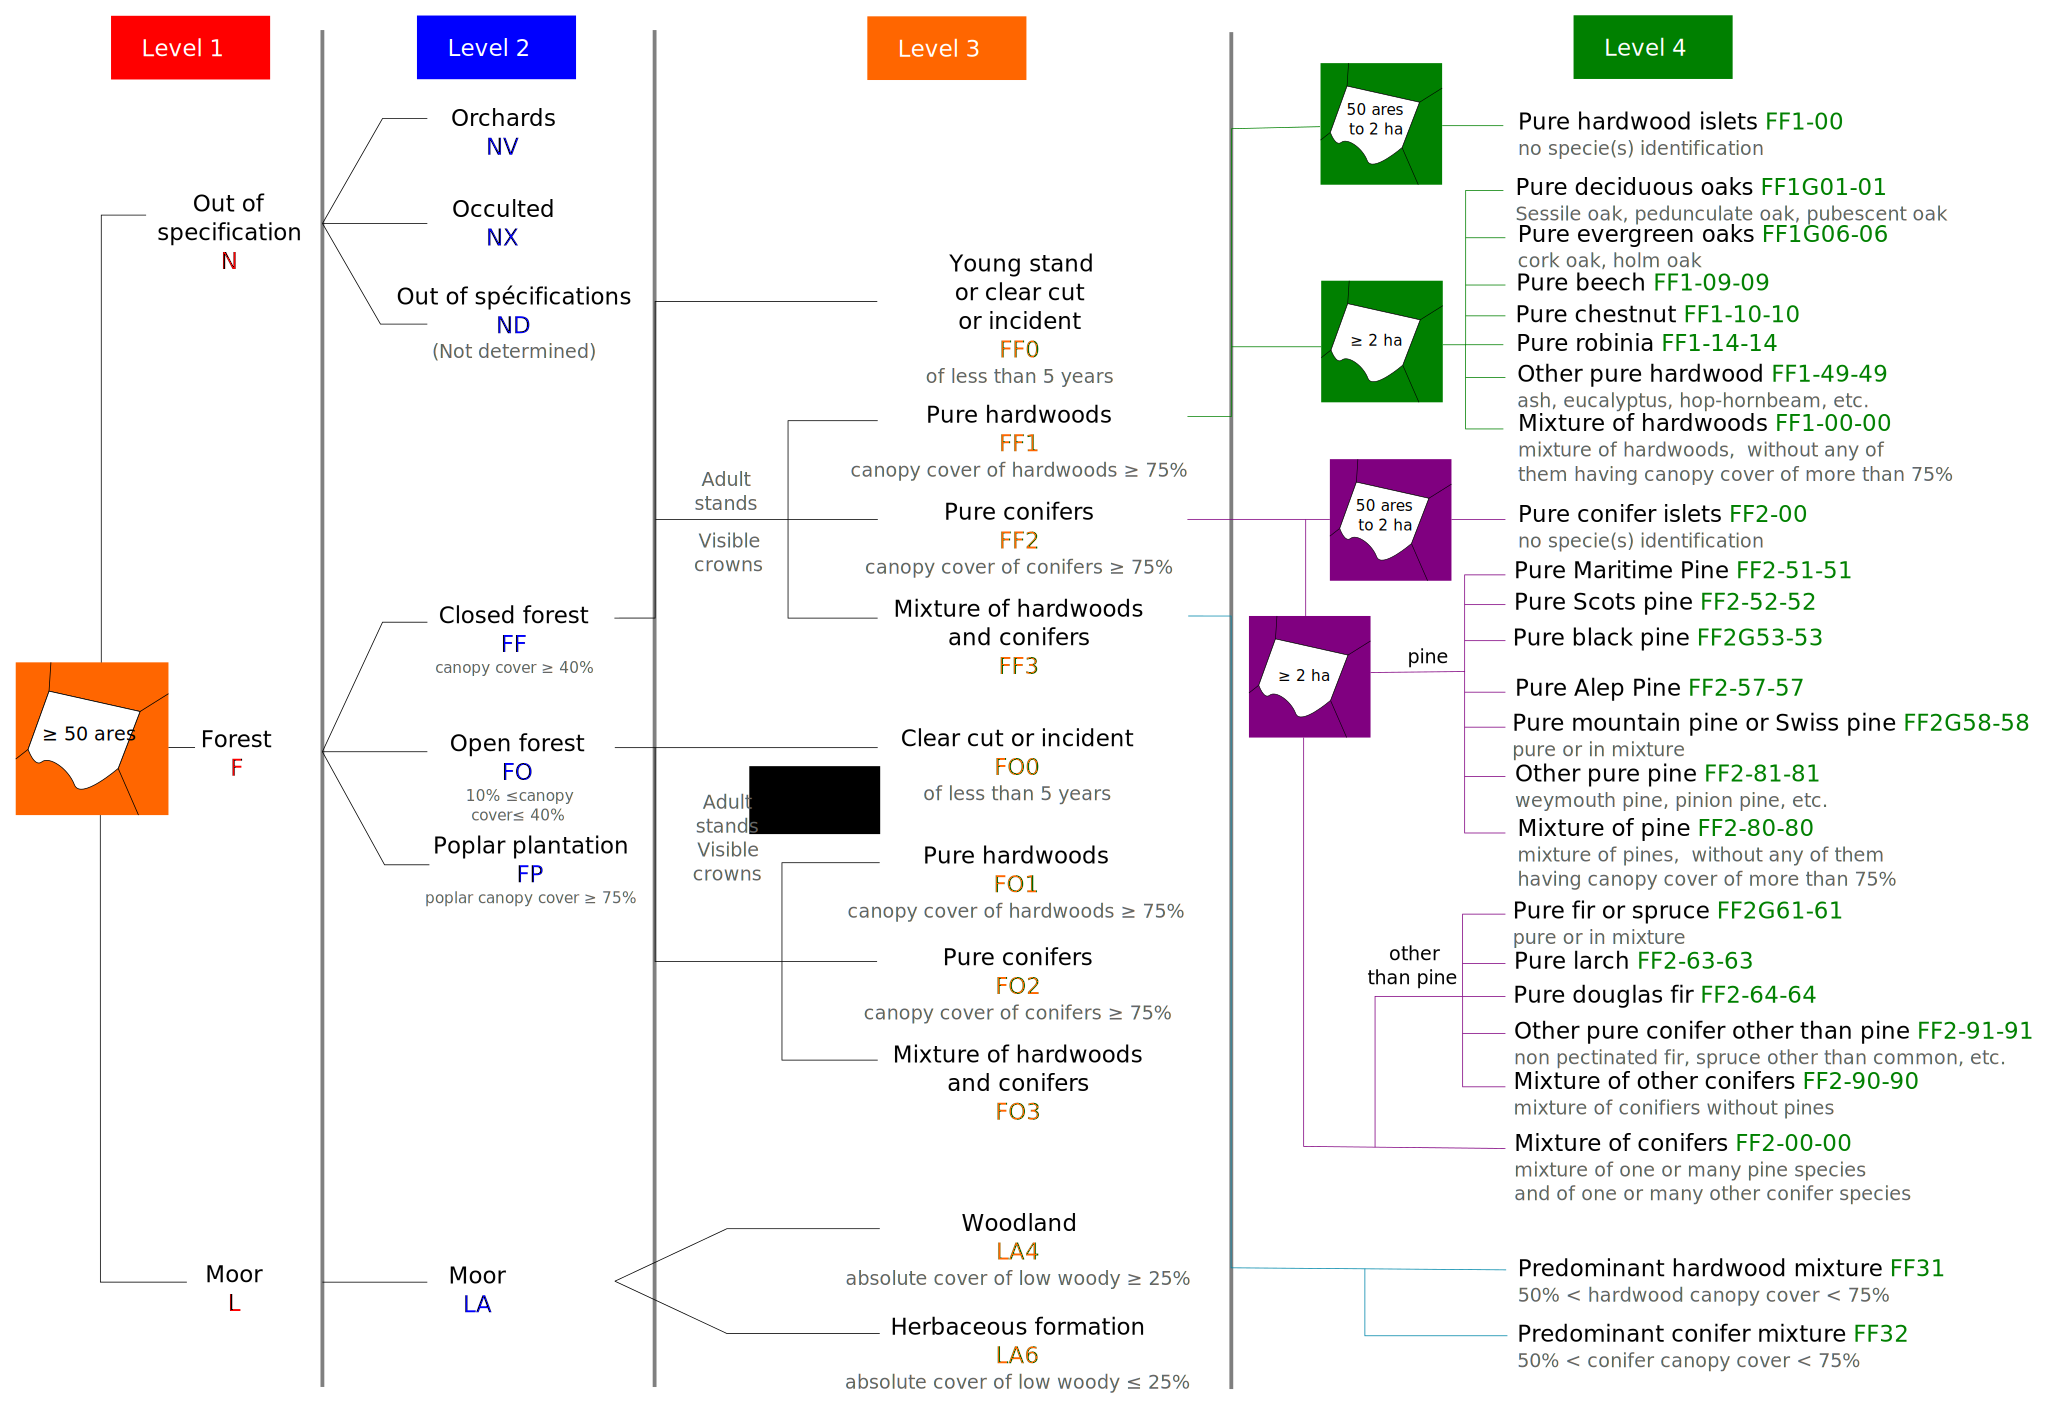
\includegraphics[width=\textwidth]{Figures/v2_organigram}
\caption{Organizational chart of the version 2 of the forest LC database.}
\label{fig:organigram_BD}
\end{center}
\end{figure}


\section{Segmentation methods}
A naive method to retrieve forest stands is to segment the input data. Such segmentation algorithms do not take into account the species information. Two algorithms were employed in order to obtain relevant stands only through the segmentation of the data.
The first segmentation algorithm is the one proposed in \cite{guigues2006scale}. It is a hierarchical segmentation algorithm that allows to control the level of segmentation through a unique scale parameter $\mu$.

The second segmentation algorithm (called here PFF) employed is presented in \cite{felzenszwalb2004efficient}. It is a method for image segmentation based on pairwise region comparison considering the minimum weight edge between two regions in measuring the difference between them. 3 simples parameters need to be tuned in order to obtain relevant segmentation. $\sigma$ is the standard deviation of the gaussian filter employed to smooth the image as a pre-processing (the authors recommend $\sigma=0.8$). $k$ is a second parameter that set a scale of observation (a larger $k$ will lead to larger segments). Finally, the parameter $m$ permits to define the minimum size of a segment.

Such segmentation could allow to retrieve the stands borders easily. Furthermore, one the segmentation is performed, one can add semantic information using classification results.

These experiments have been performed only on one area presented in Figure~\ref{fig:data_direct_seg}. It is a 1$\:$km$^{2}$ area, the spatial resolution of the VHR optical image is 0.5$\:$m, and the nDSM has been rasterized at the same resolution. From these data one can see that a stand is composed of zones that are not homogeneous in term of reflectance and/or height. Furthermore, one can also note that the variability between two stands in terms of reflectance and/or height might not be important.

\begin{figure}[htbp]
\begin{center}
\begingroup
\captionsetup[subfigure]{width=0.16\textwidth}
\subfloat[VHR IRC optical image.]{
\includegraphics[width=0.3\textwidth]{Figures/C3/S2/IRC}
\label{subfig:data_direct_sega}
}
\subfloat[nDSM.]{
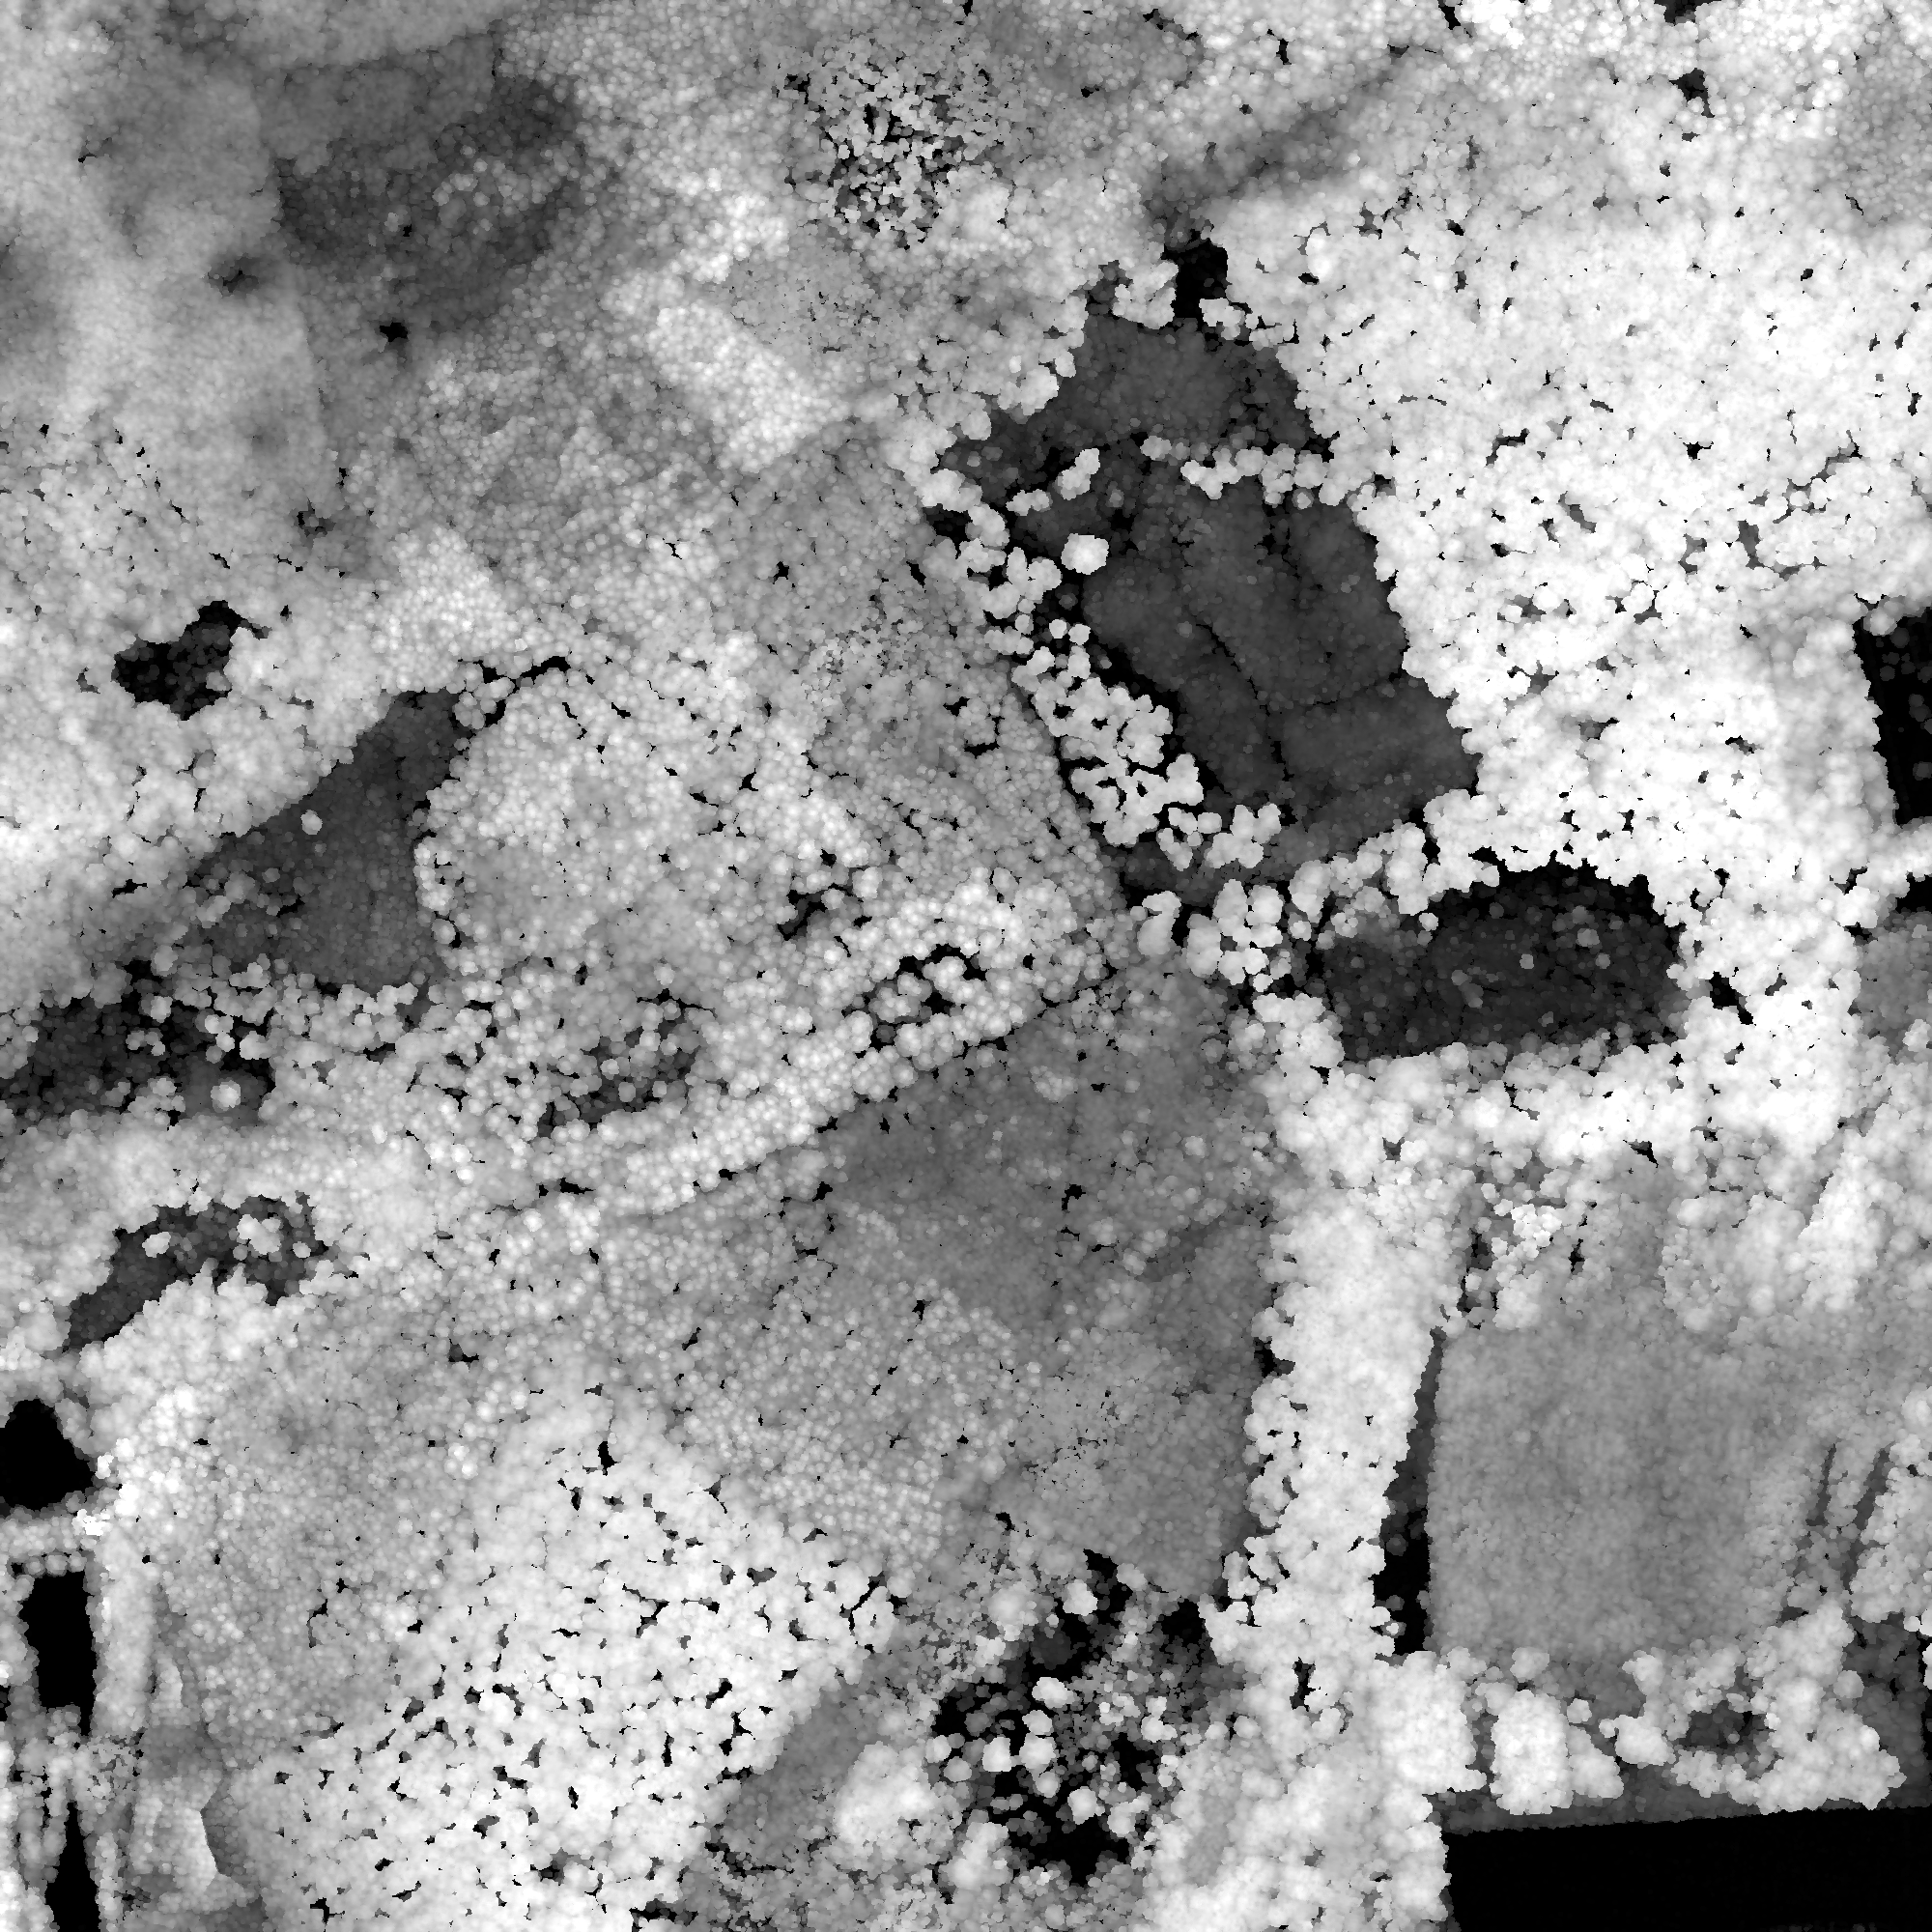
\includegraphics[width=0.3\textwidth]{Figures/C3/S2/nDSM}
\label{subfig:data_direct_segb}
}
\subfloat[Forest LC database.]{
\includegraphics[width=0.3\textwidth]{Figures/C3/S2/BD}
\label{subfig:data_direct_segc}
}
\endgroup
\caption{VHR IRC optical image, rasterized nDSM and forest LC of the proposed area for the direct segmentation tests.}
\label{fig:data_direct_seg}
\end{center}
\end{figure}

\subsection{Retrieve stands borders}
\label{sec:C3_S2_ss1}
Two strategies are employed to apply the segmentation in order to retrieve the forest stands borders from the forest LC database:
\begin{itemize}
\item The segmentation is applied to the VHR optical images, thus the resulting segment will correspond to "stands" that are homogeneous in terms of spectral reflectance. Since the optical images are employed by photo-interpreters in order to derive the forest LC, such segmentation should produce results similar to the forest LC.
\item The segmentation is also applied to the rasterized normalized digital surface model (nDSM) (canopy height without ground relief). Such segmentation would produce "stands" that are homogeneous in term of height.
\end{itemize}

The results of the segmentation of the VHR optical image using the two segmentation algorithm is presented in Figure~\ref{fig:seg_im}. In both cases, most of the borders found are not consistent with the forest LC database. Visually, the hierarchical segmentation seems to be more relevant than the PFF segmentation. However, the hierarchical segmentation produces small segments due to high variation of illumination in the image, while the PFF segments are all relatively large. 

\begin{figure}[htbp]
\begin{center}
\begingroup
\captionsetup[subfigure]{width=0.4\textwidth}
\subfloat[Hierarchical segmentation with $\mu=15$.]{
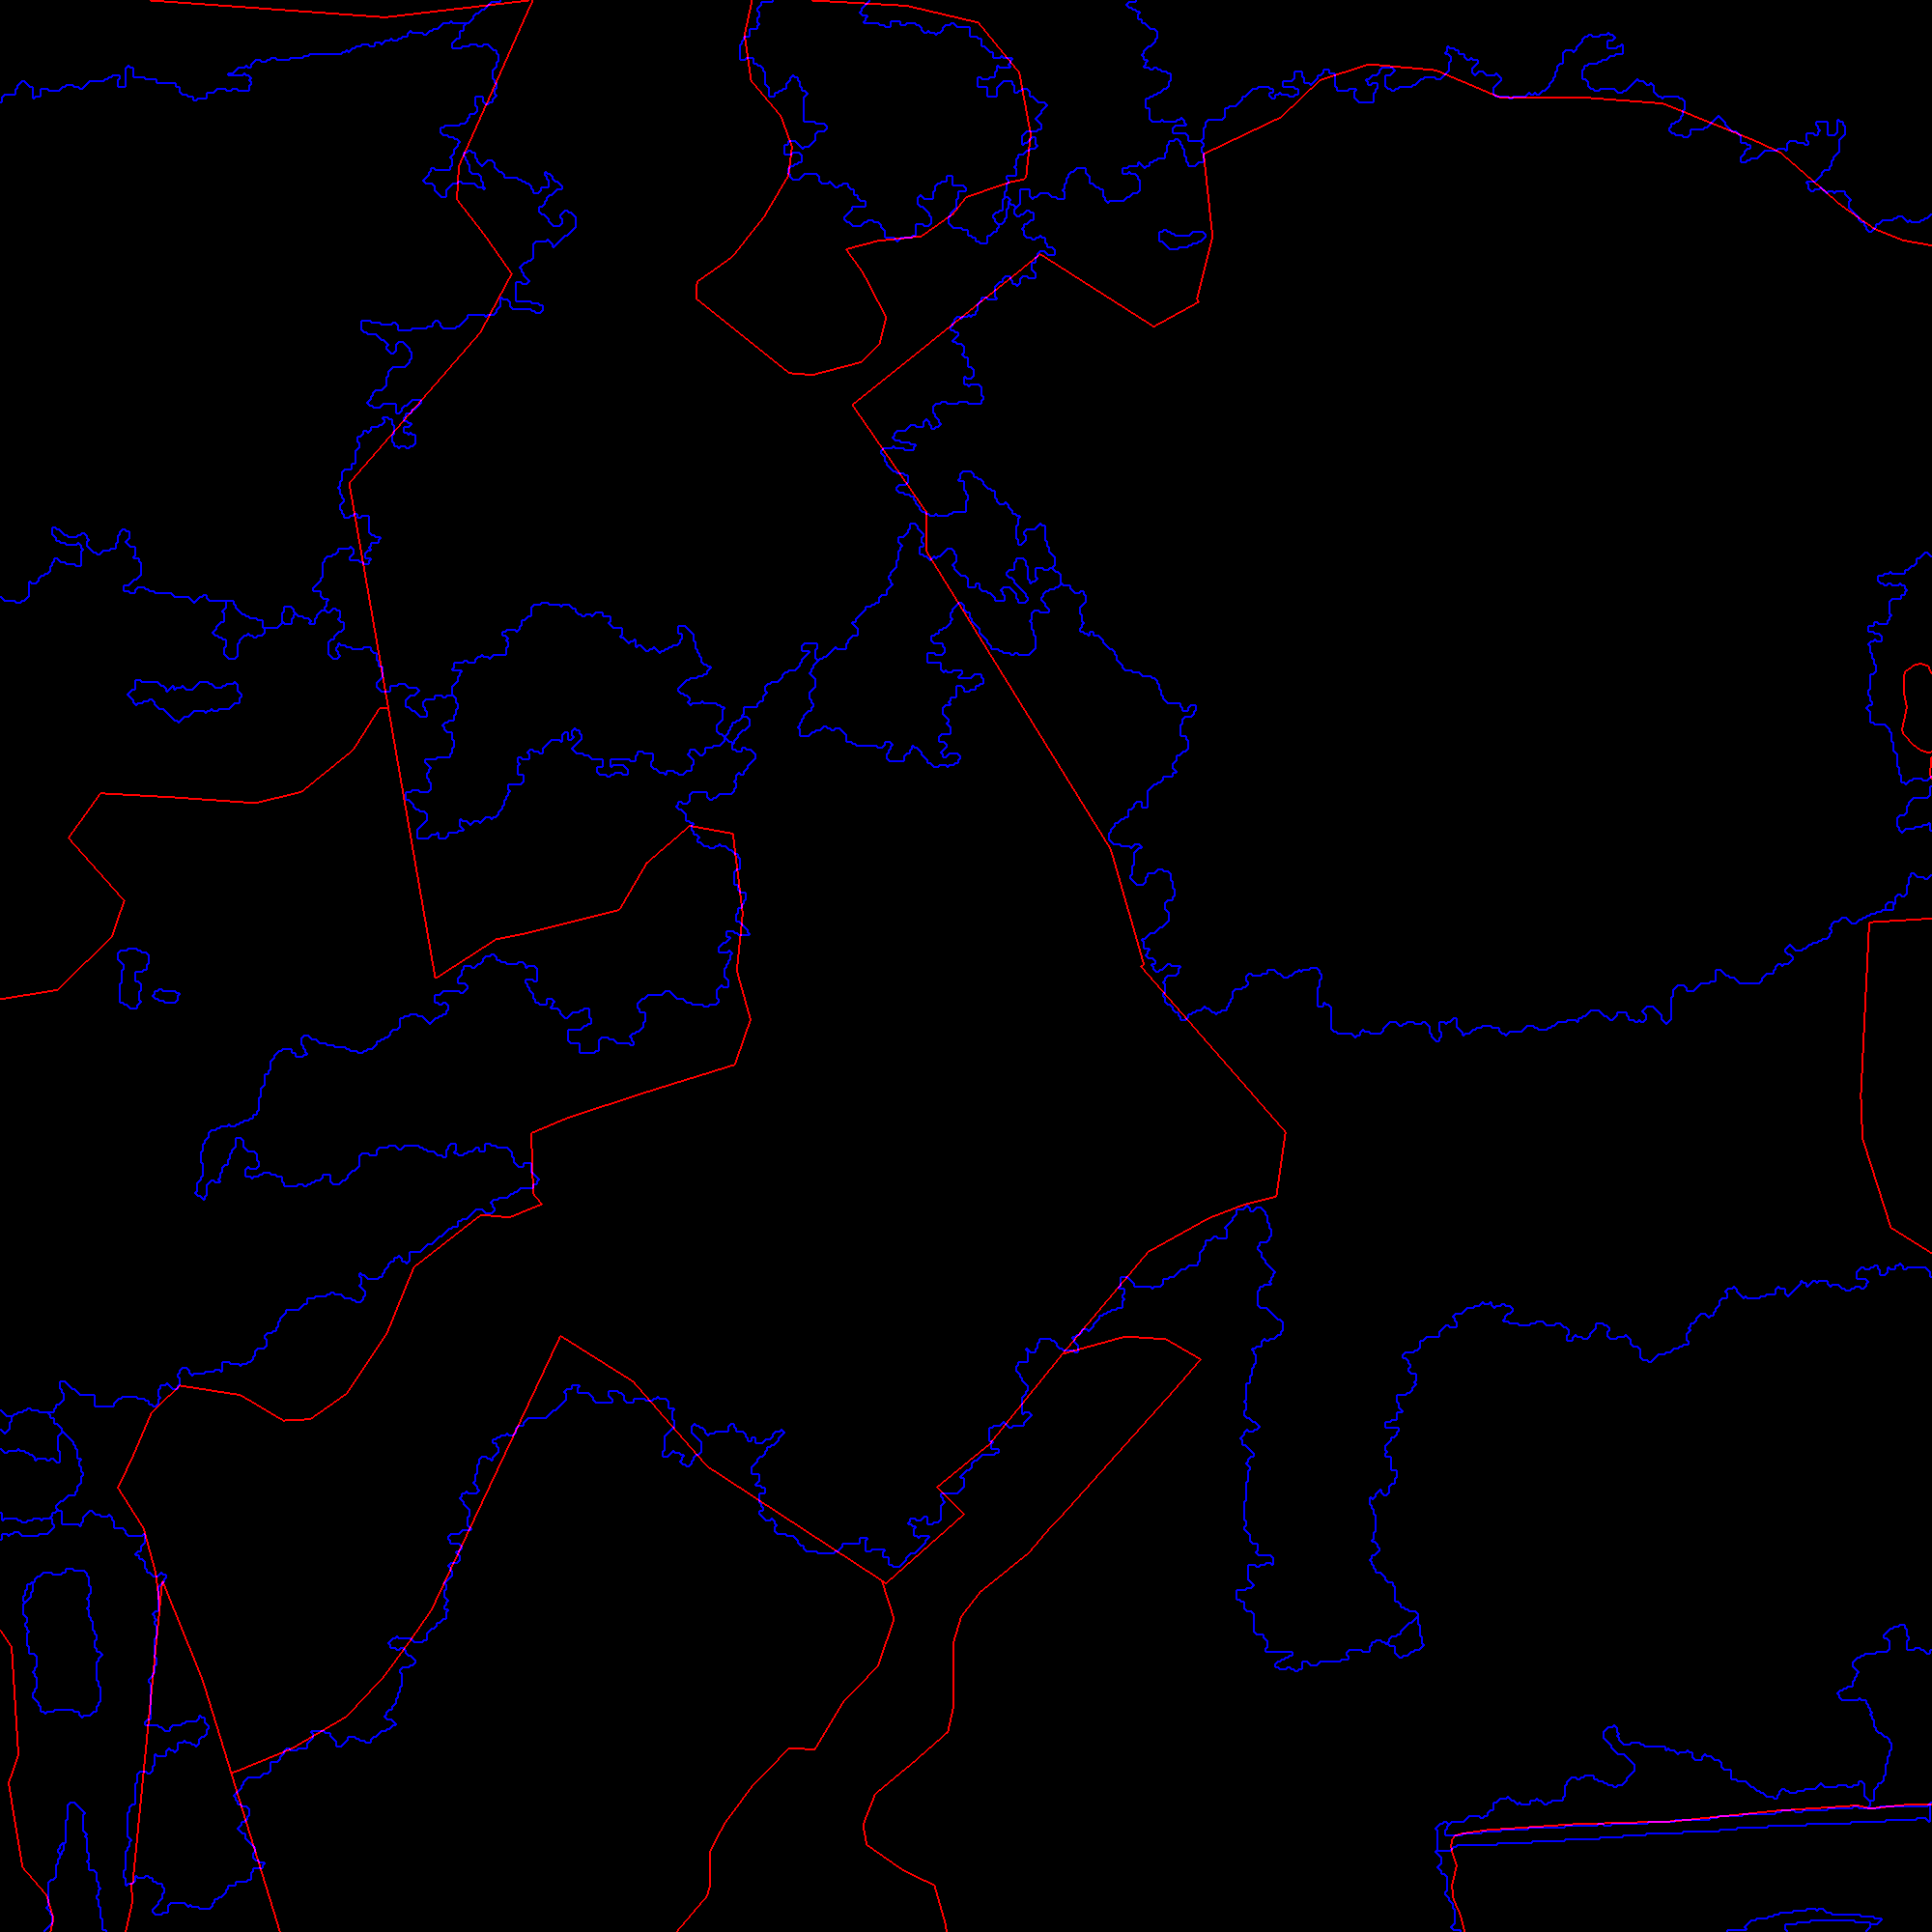
\includegraphics[width=0.45\textwidth]{Figures/C3/S2/border_hierar}
\label{subfig:seg_ima}
}
\hspace*{0.05\textwidth}
\subfloat[PFF segmentation with $\sigma=0.8$, $k=500$ and $m=40000$.]{
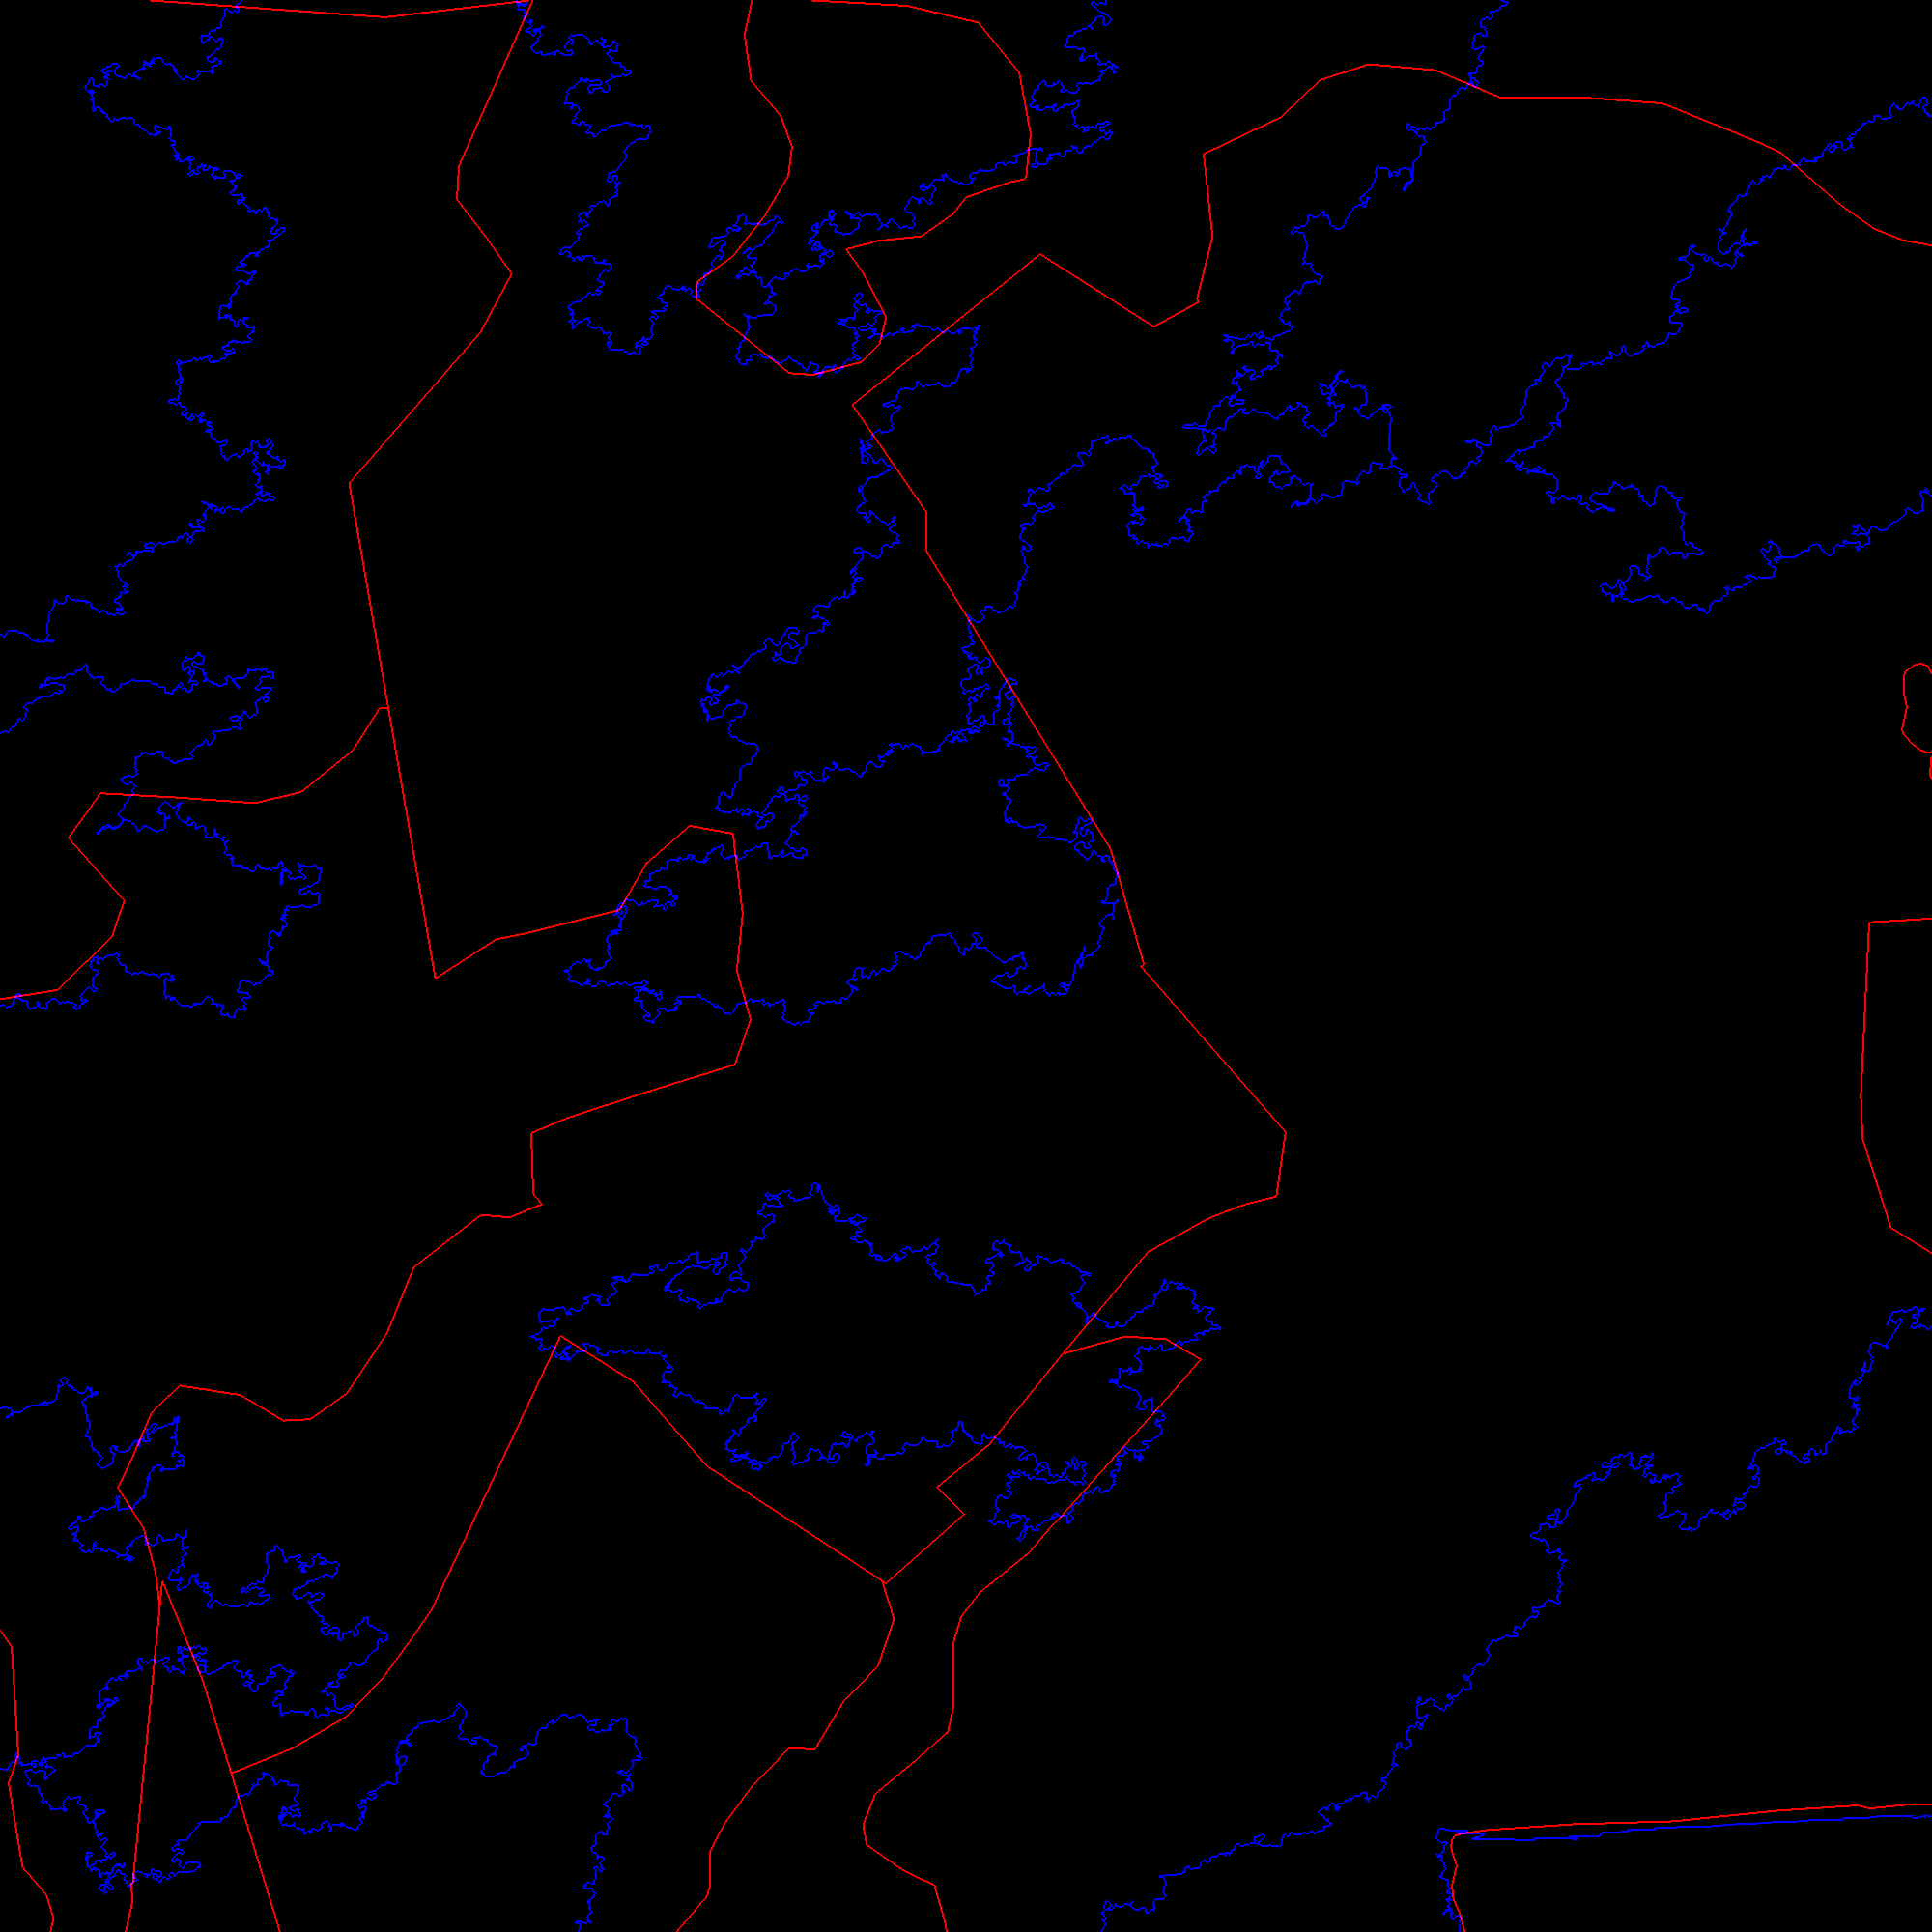
\includegraphics[width=0.45\textwidth]{Figures/C3/S2/border_PFF_IRC}
\label{subfig:seg_imb}
}
\endgroup
\caption{Result of the segmentation of the VHR optical image for the two segmentation algorithms. Blue lines correspond to the borders of the segments, red lines correspond to the borders of the forest LC.}
\label{fig:seg_im}
\end{center}
\end{figure}

The results of the segmentation of rasterized nDSM using the two segmentation algorithm is presented in Figure~\ref{fig:seg_nDSM}. Just like the segmentation of the VHR optical image, most of the borders found are not consistent with the forest LC database. Here, the PFF segmentation seems to perform better than the hierarchical segmentation visually.


\begin{figure}[htbp]
\begin{center}
\begingroup
\captionsetup[subfigure]{width=0.4\textwidth}
\subfloat[Hierarchical segmentation with $\mu=15$.]{
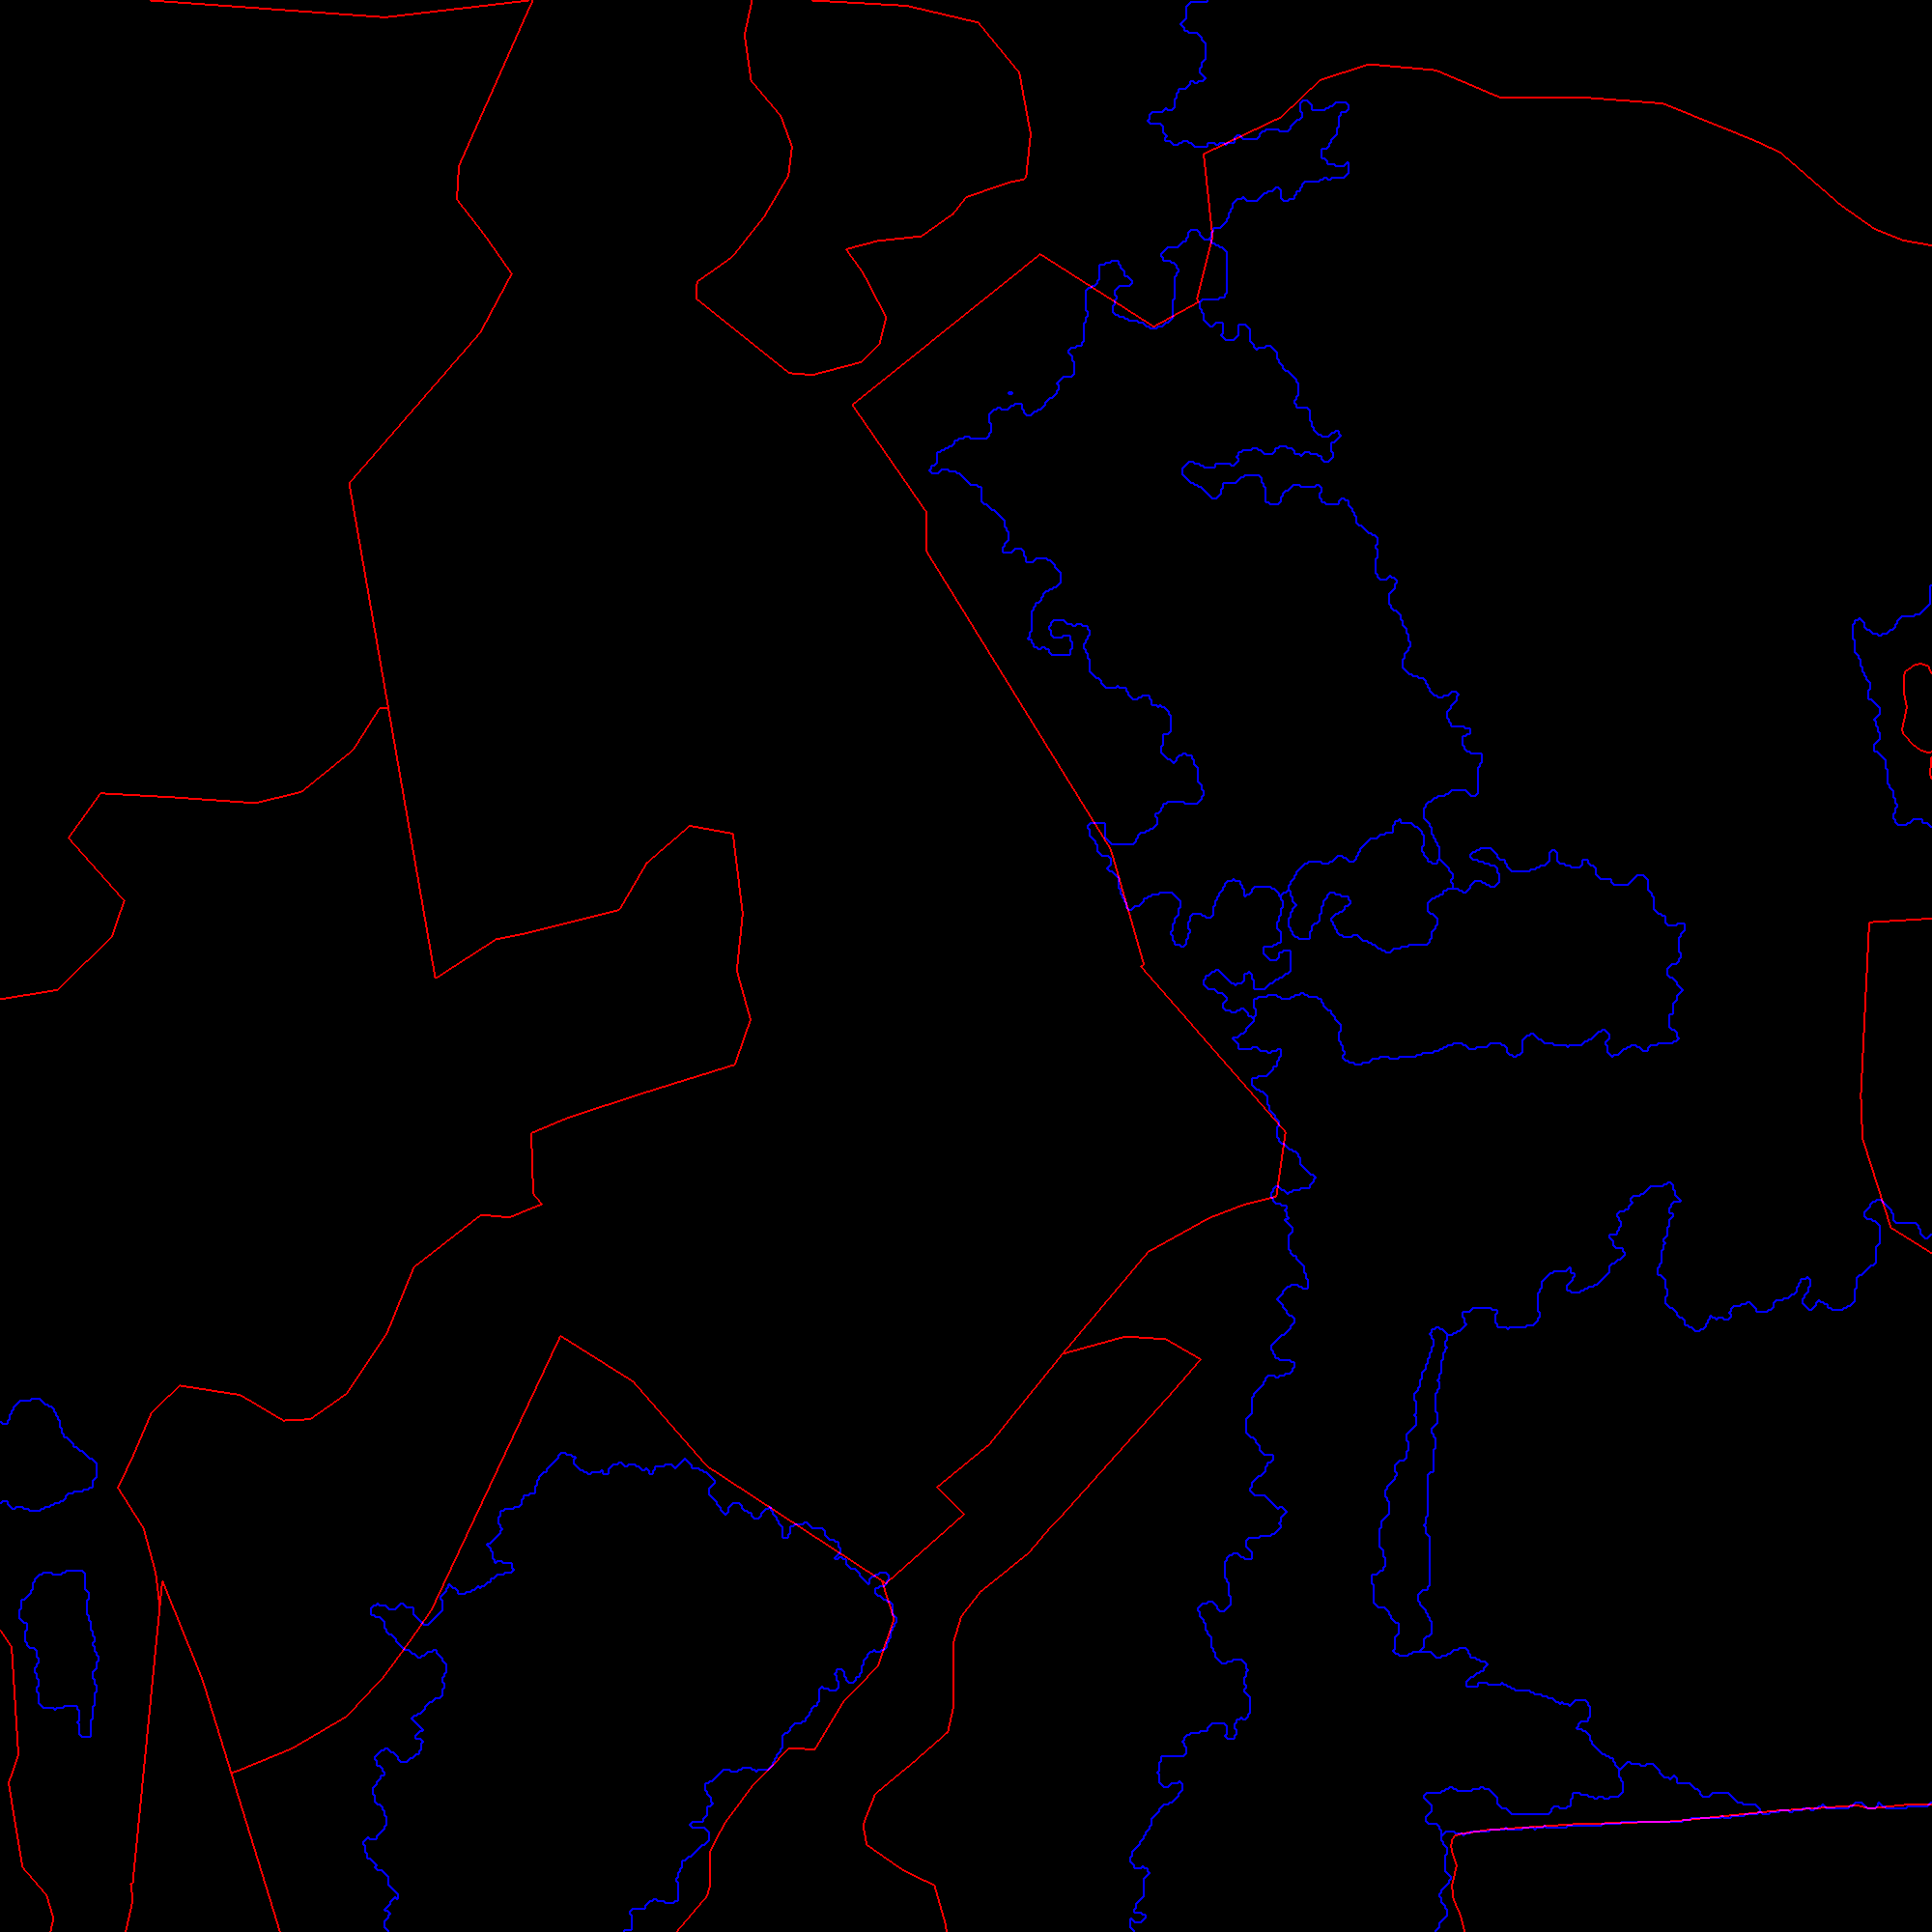
\includegraphics[width=0.45\textwidth]{Figures/C3/S2/border_hierar_z}
\label{subfig:seg_nDSMa}
}
\hspace*{0.05\textwidth}
\subfloat[PFF segmentation with $\sigma=0.8$, $k=500$ and $m=40000$.]{
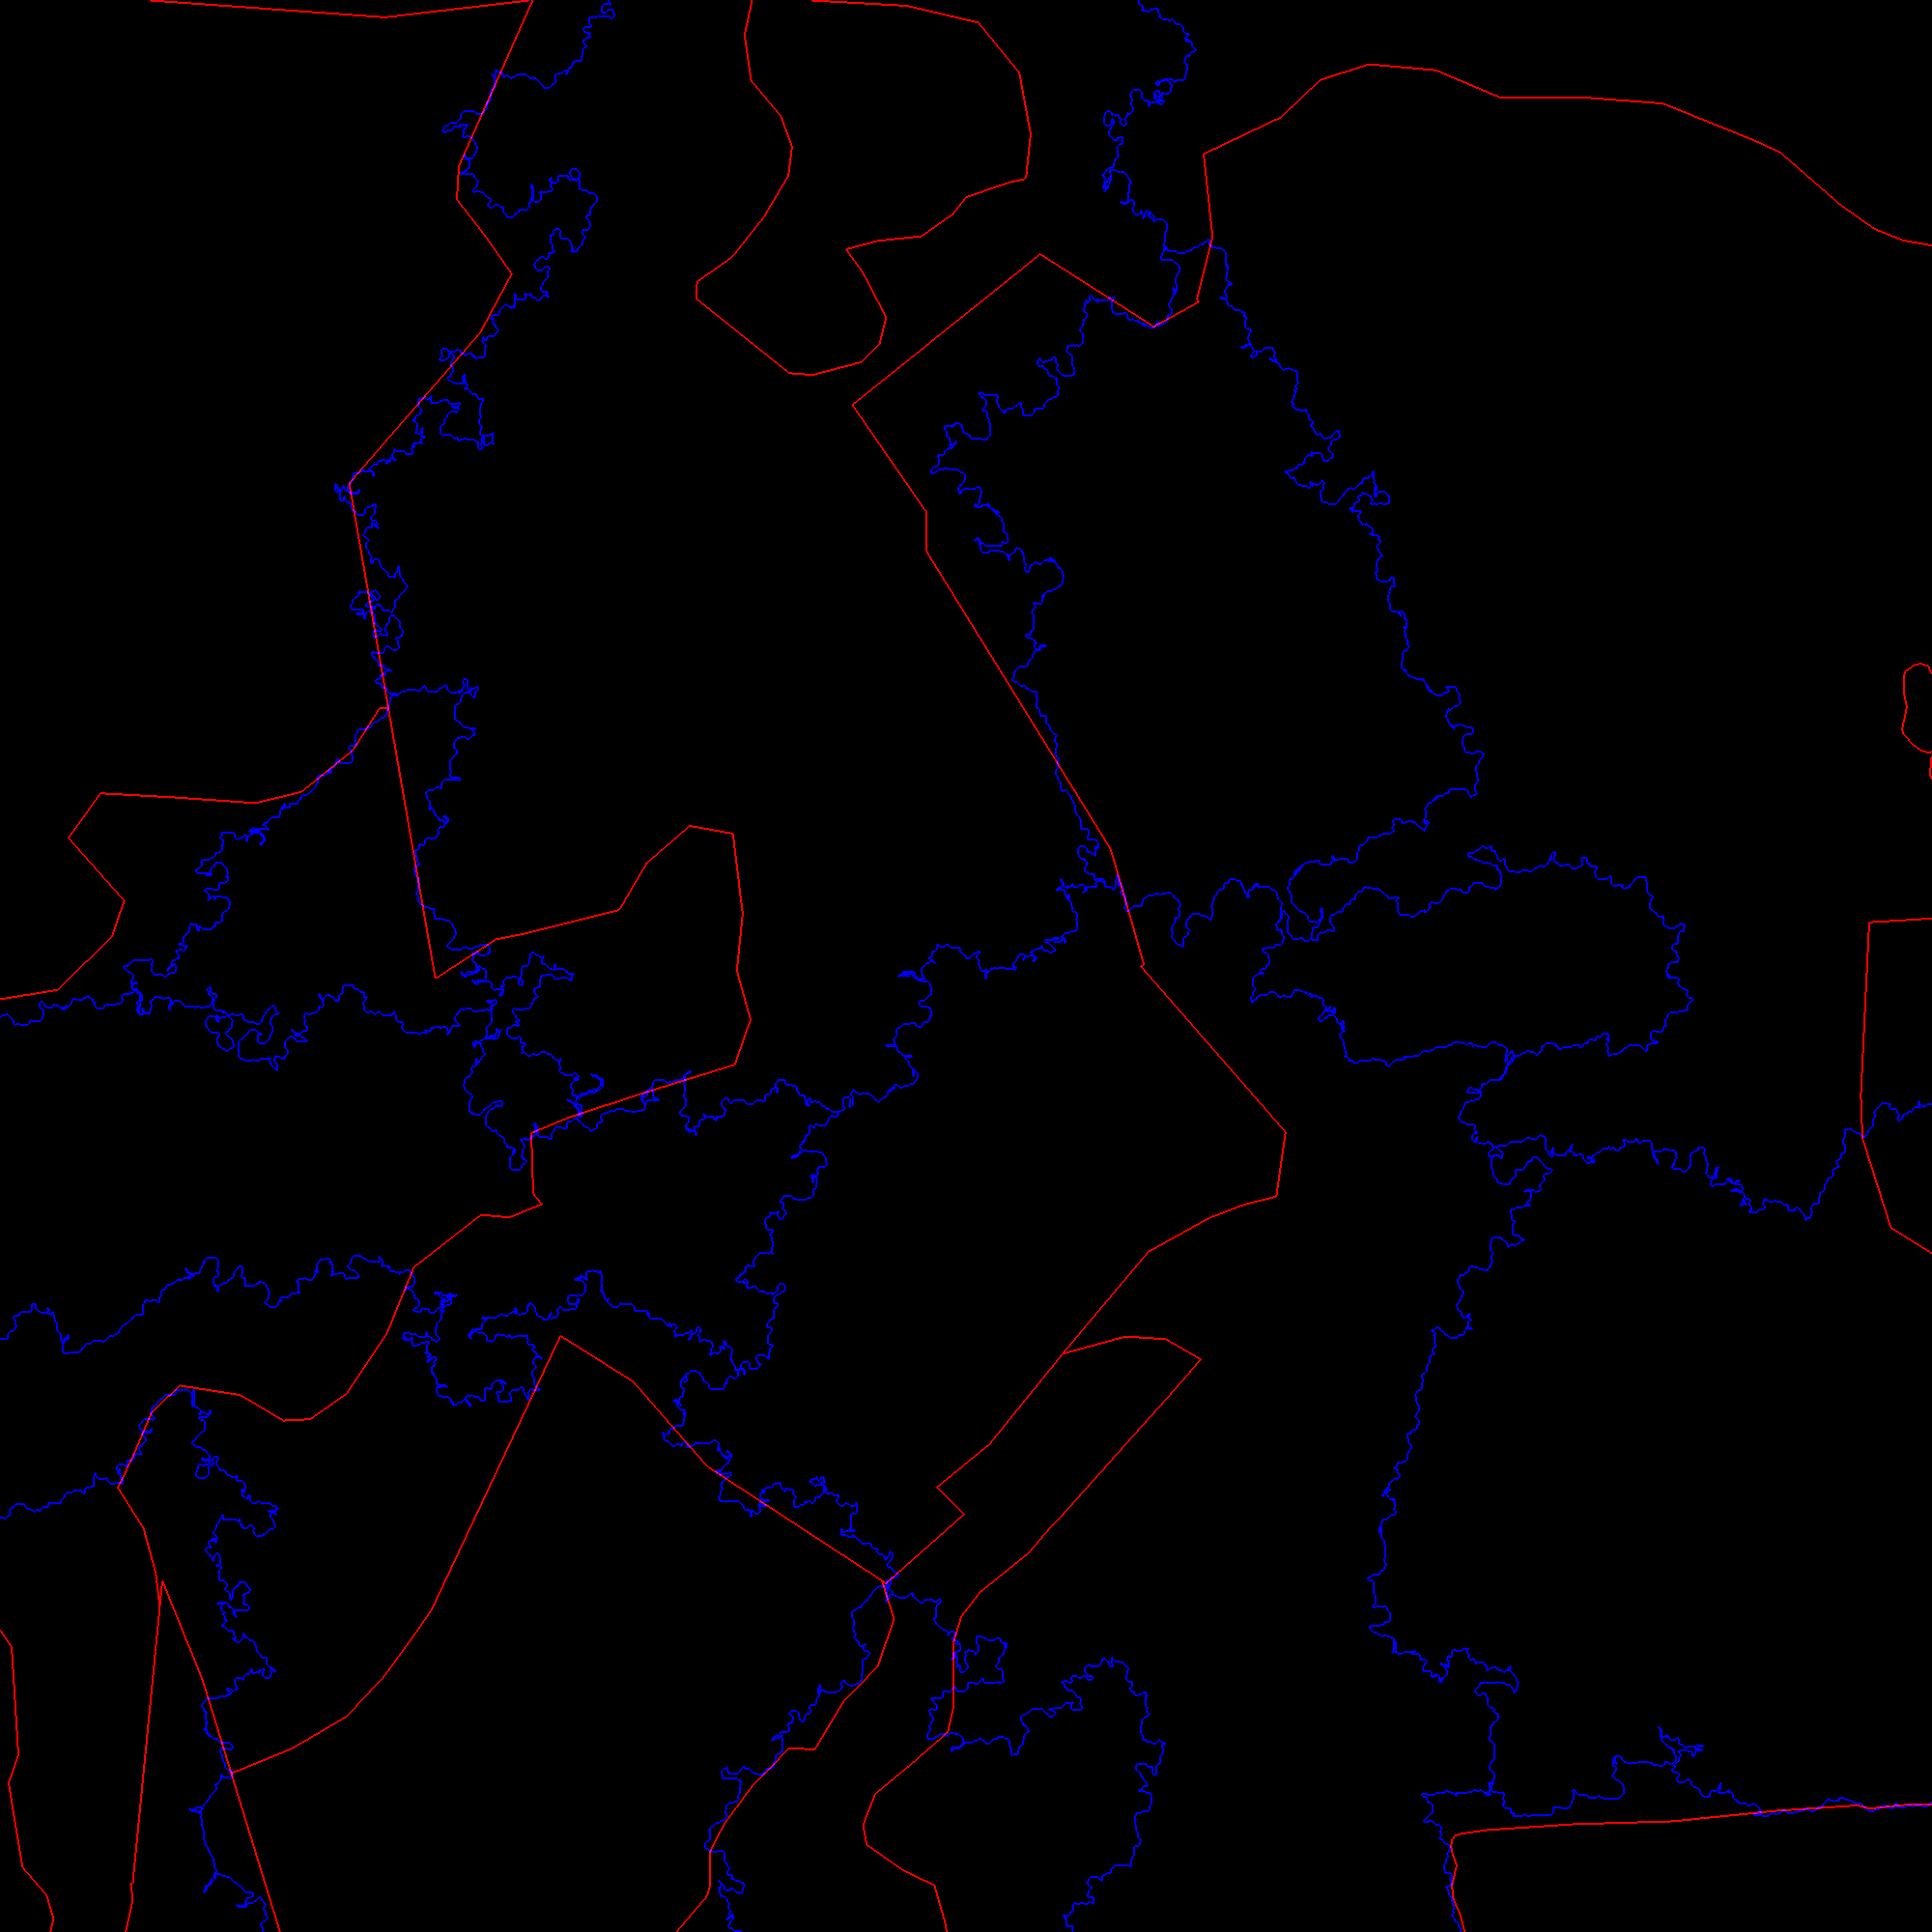
\includegraphics[width=0.45\textwidth]{Figures/C3/S2/border_PFF_z}
\label{subfig:seg_nDSMb}
}
\endgroup
\caption{Result of the segmentation of the nDSM for the two segmentation algorithms. Blue lines correspond to the borders of the segments, red lines correspond to the borders of the forest LC.}
\label{fig:seg_nDSM}
\end{center}
\end{figure}

Since the segmentation on the VHR optical image and the nDSM does not allow to retrieve the borders from the forest LC database, different values of the parameter $\mu$ for the hierarchical segmentation on the VHR optical images (see Figure~\ref{fig:hierar}). It appears that decreasing $\mu$ does not allow to obtain the borders of the forest LC. It only leads to and over-segmentation of the image. Such over-segmentation is employed in the proposed method but is not employed as a relevant segmentation for stand delineation but as an input for object based classification.

\begin{figure}[htbp]
\begin{center}
\begingroup
\captionsetup[subfigure]{width=0.5\textwidth}
\subfloat[Hierarchical segmentation with $\mu=3$.]{
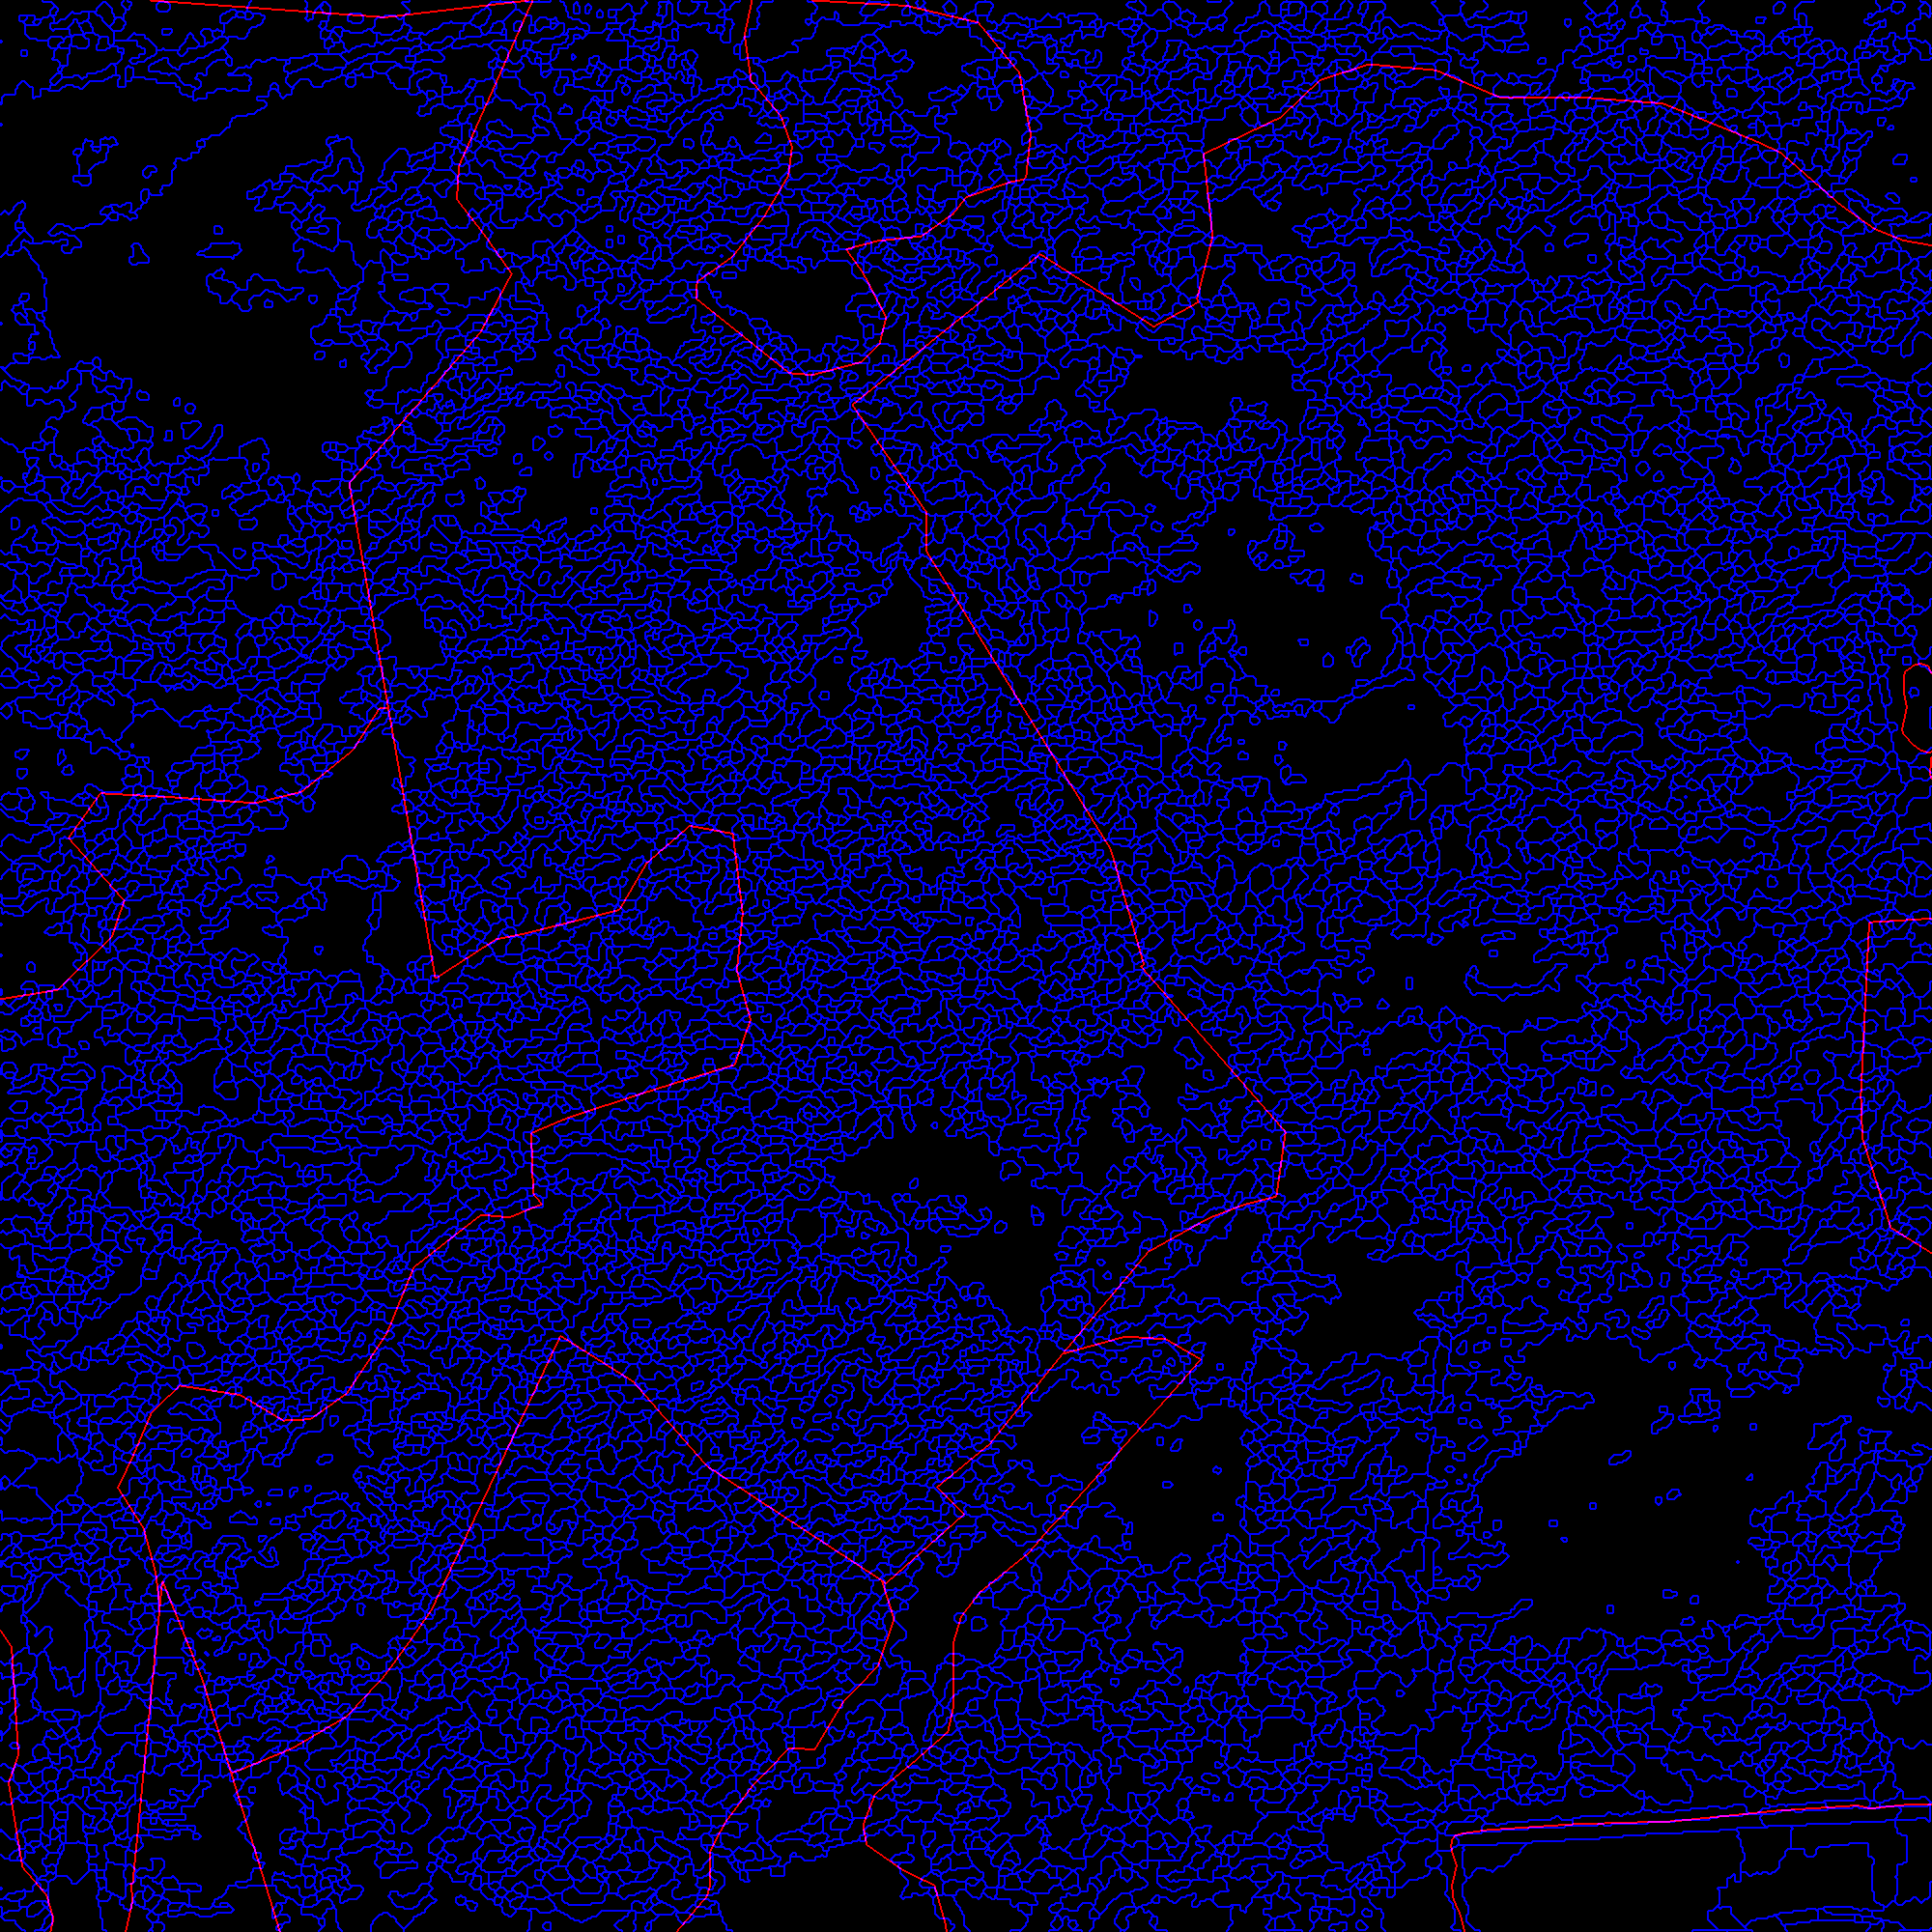
\includegraphics[width=0.45\textwidth]{Figures/C3/S2/seg_herarchical_3border_hierarchical}
\label{subfig:hierar3}
}
\hspace*{0.05\textwidth}
\subfloat[Hierarchical segmentation with $\mu=6$.]{
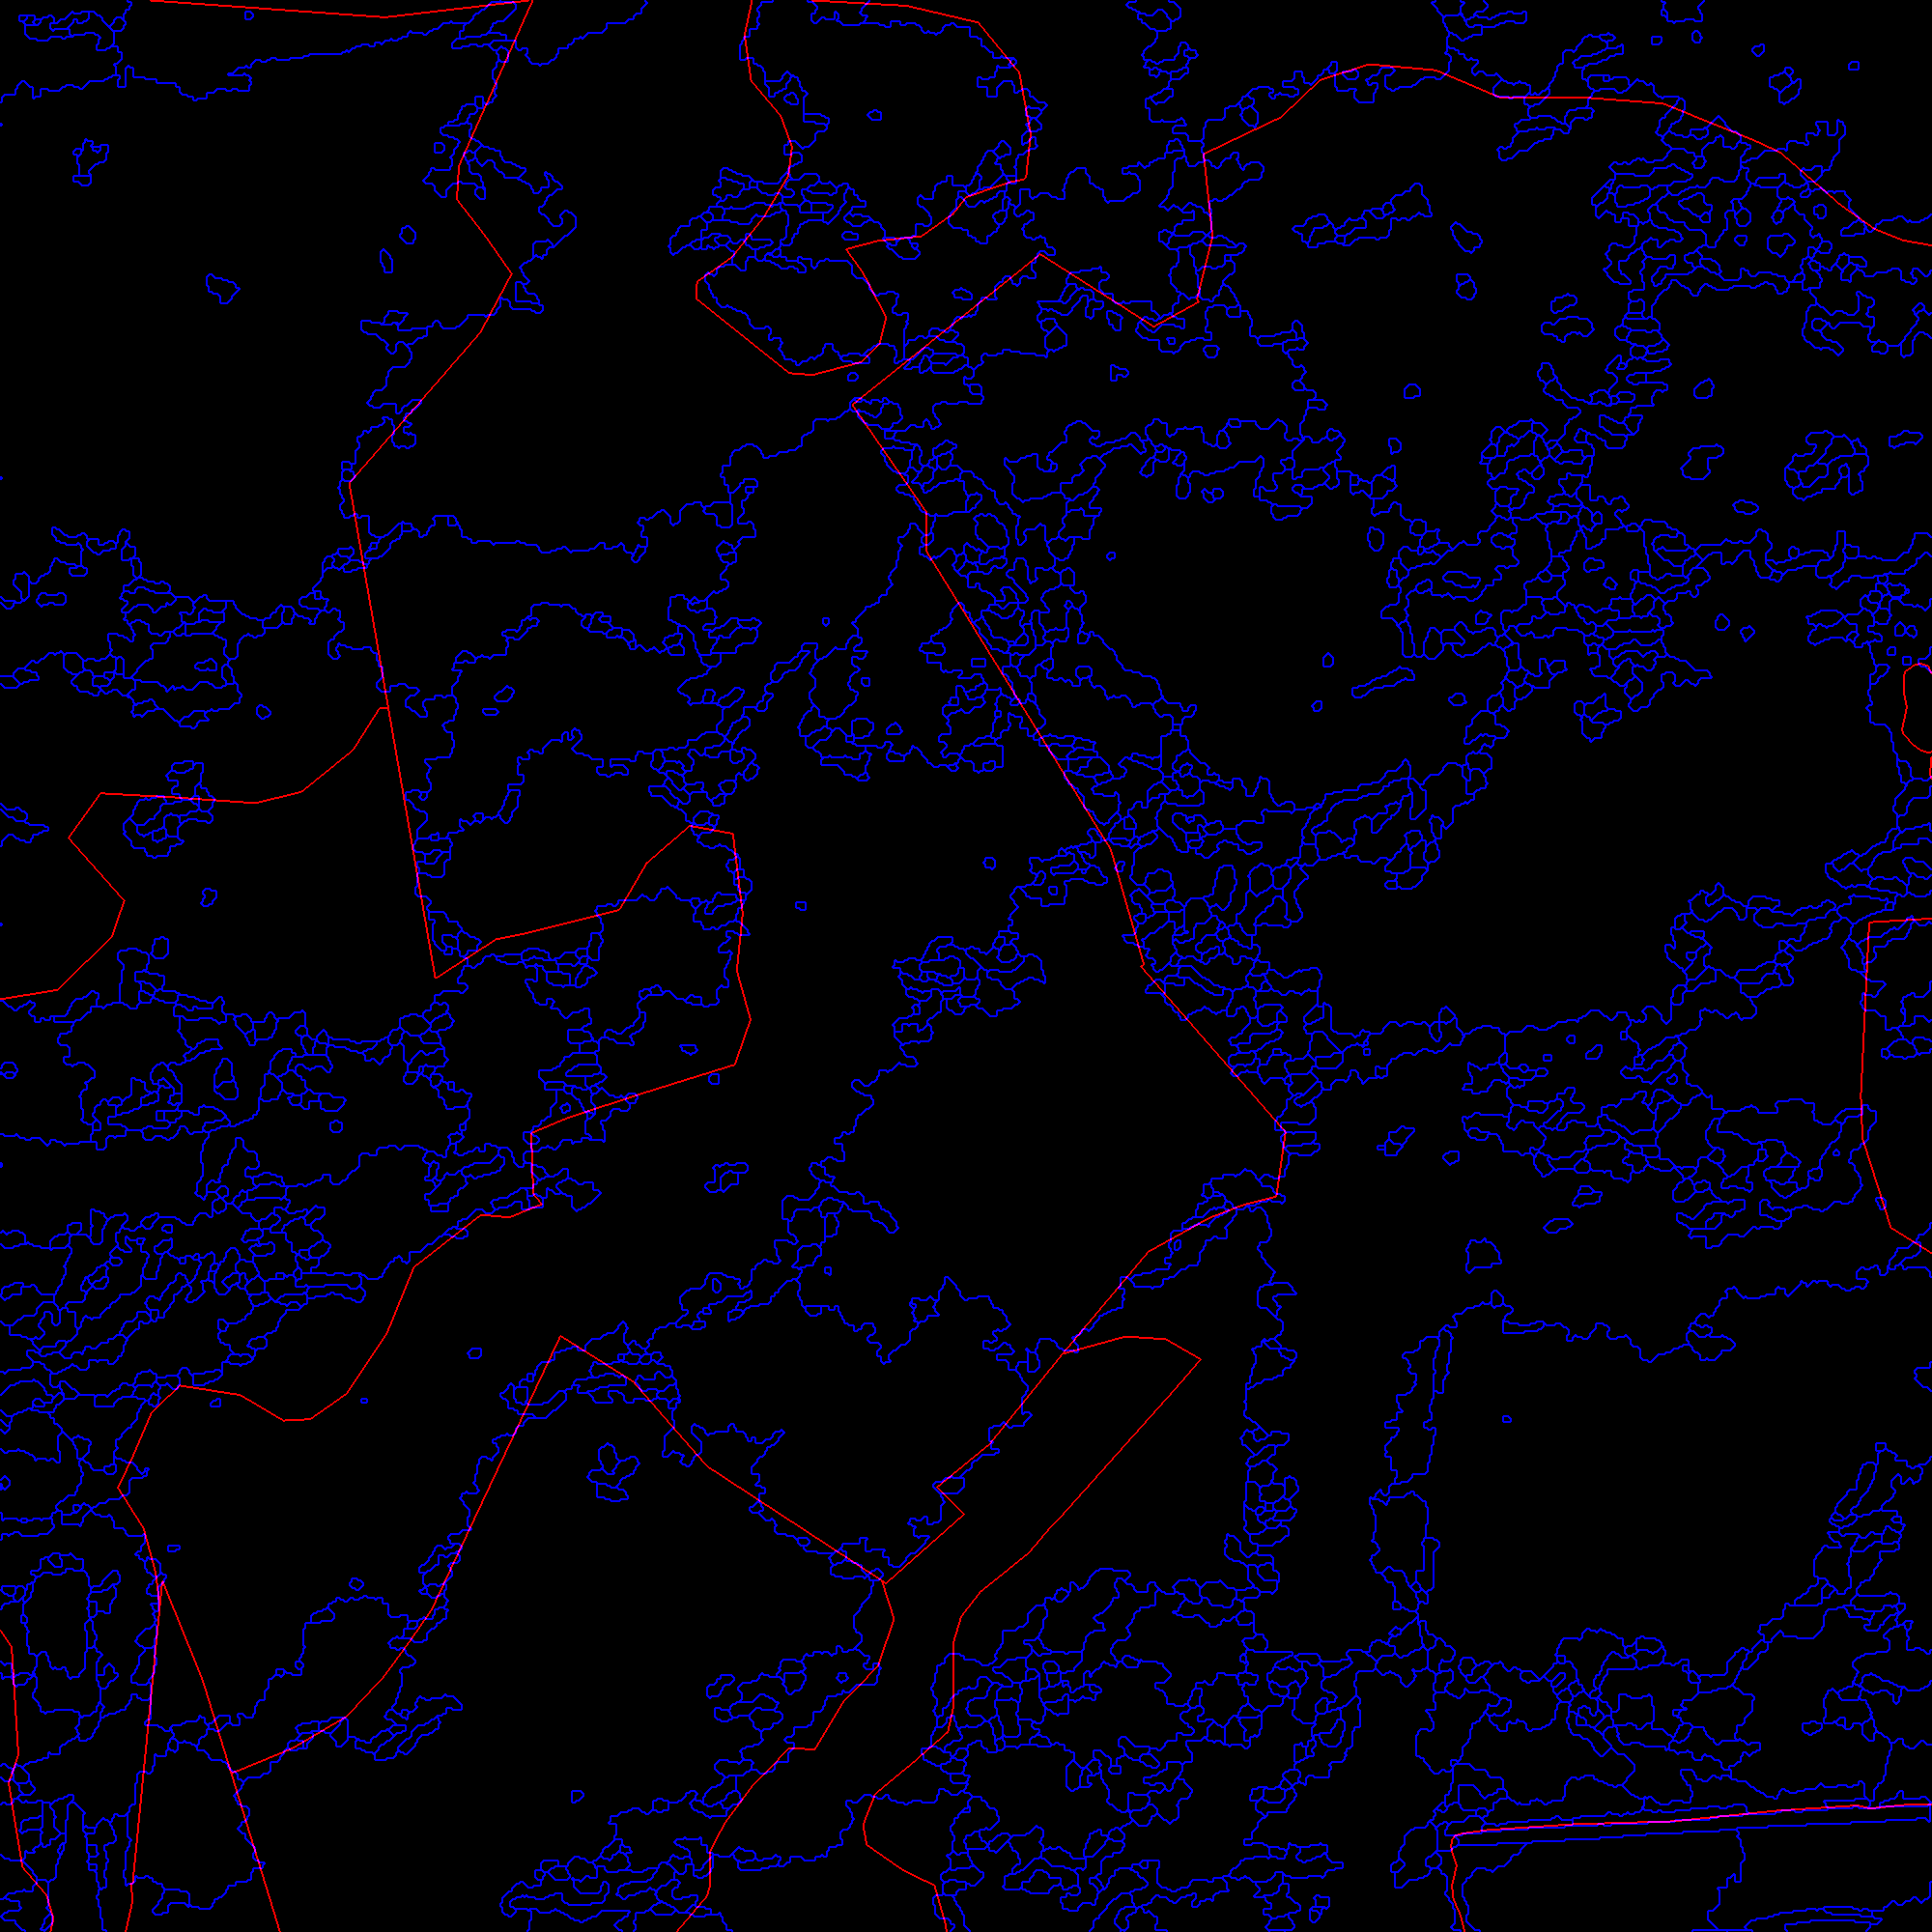
\includegraphics[width=0.45\textwidth]{Figures/C3/S2/seg_herarchical_6border_hierarchical}
\label{subfig:hierar6}
}
\\
\subfloat[Hierarchical segmentation with $\mu=8$.]{
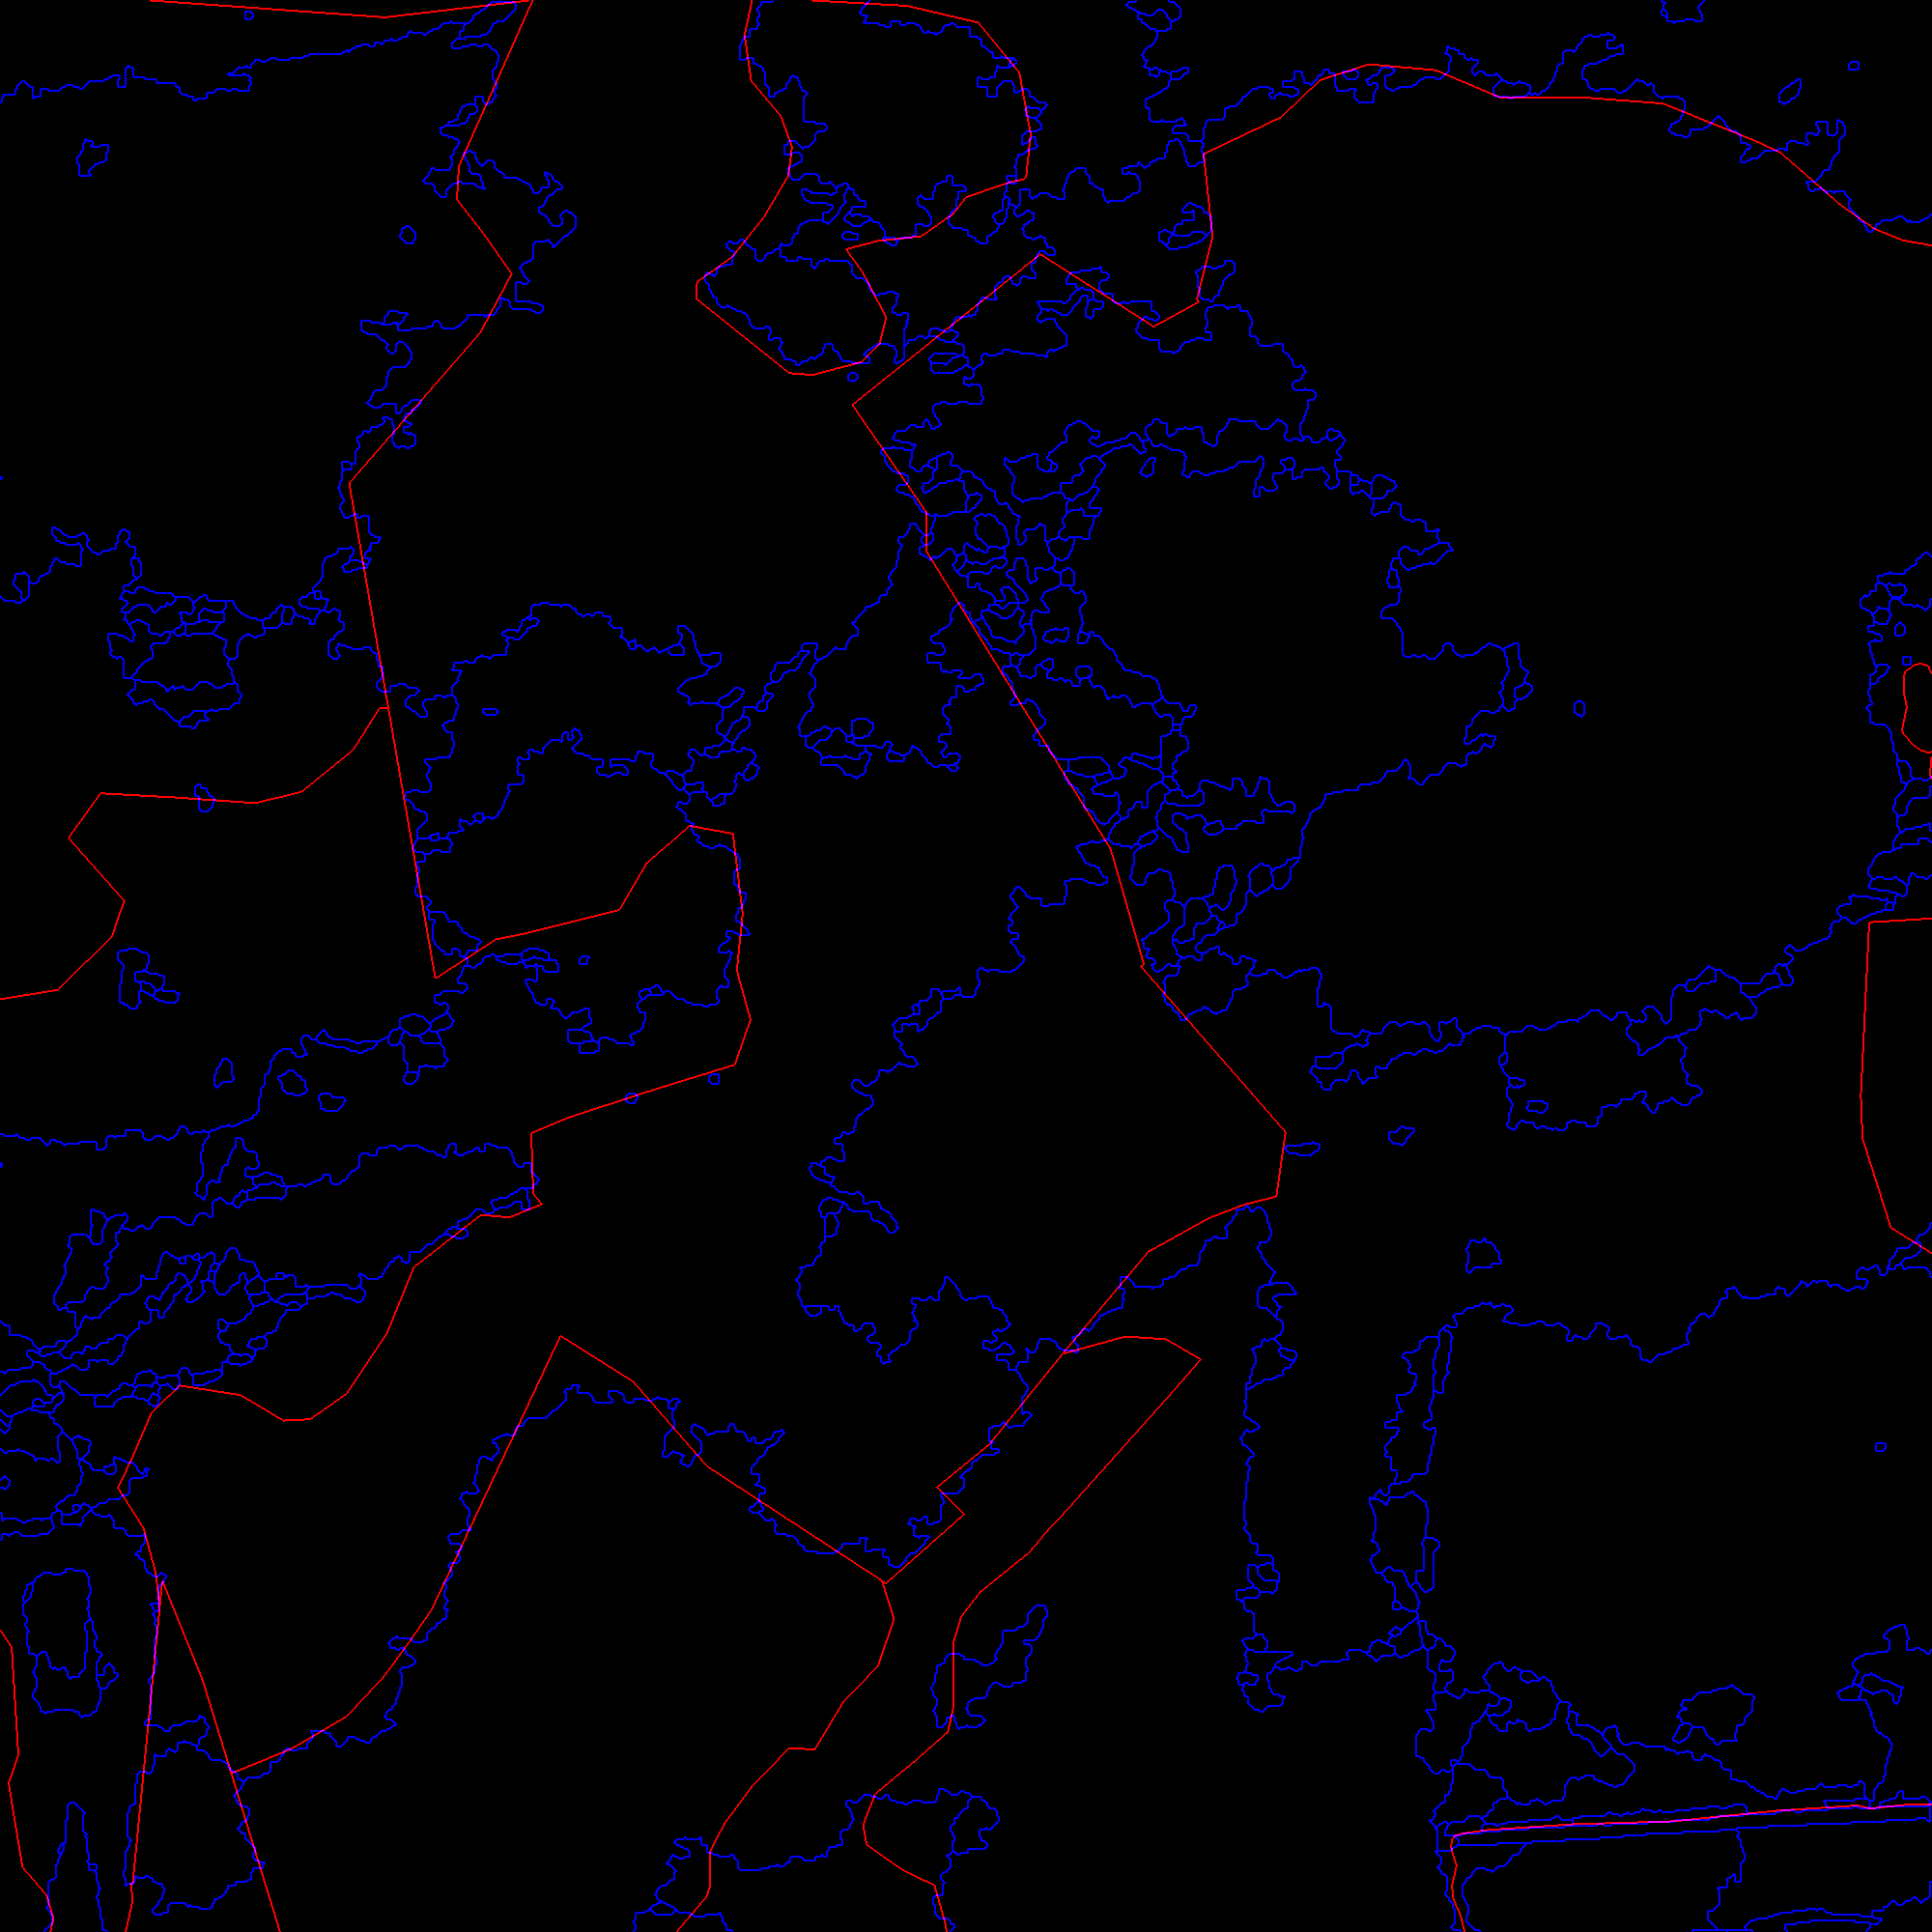
\includegraphics[width=0.45\textwidth]{Figures/C3/S2/seg_herarchical_8border_hierarchical}
\label{subfig:hierar8}
}
\hspace*{0.05\textwidth}
\subfloat[Hierarchical segmentation with $\mu=10$.]{
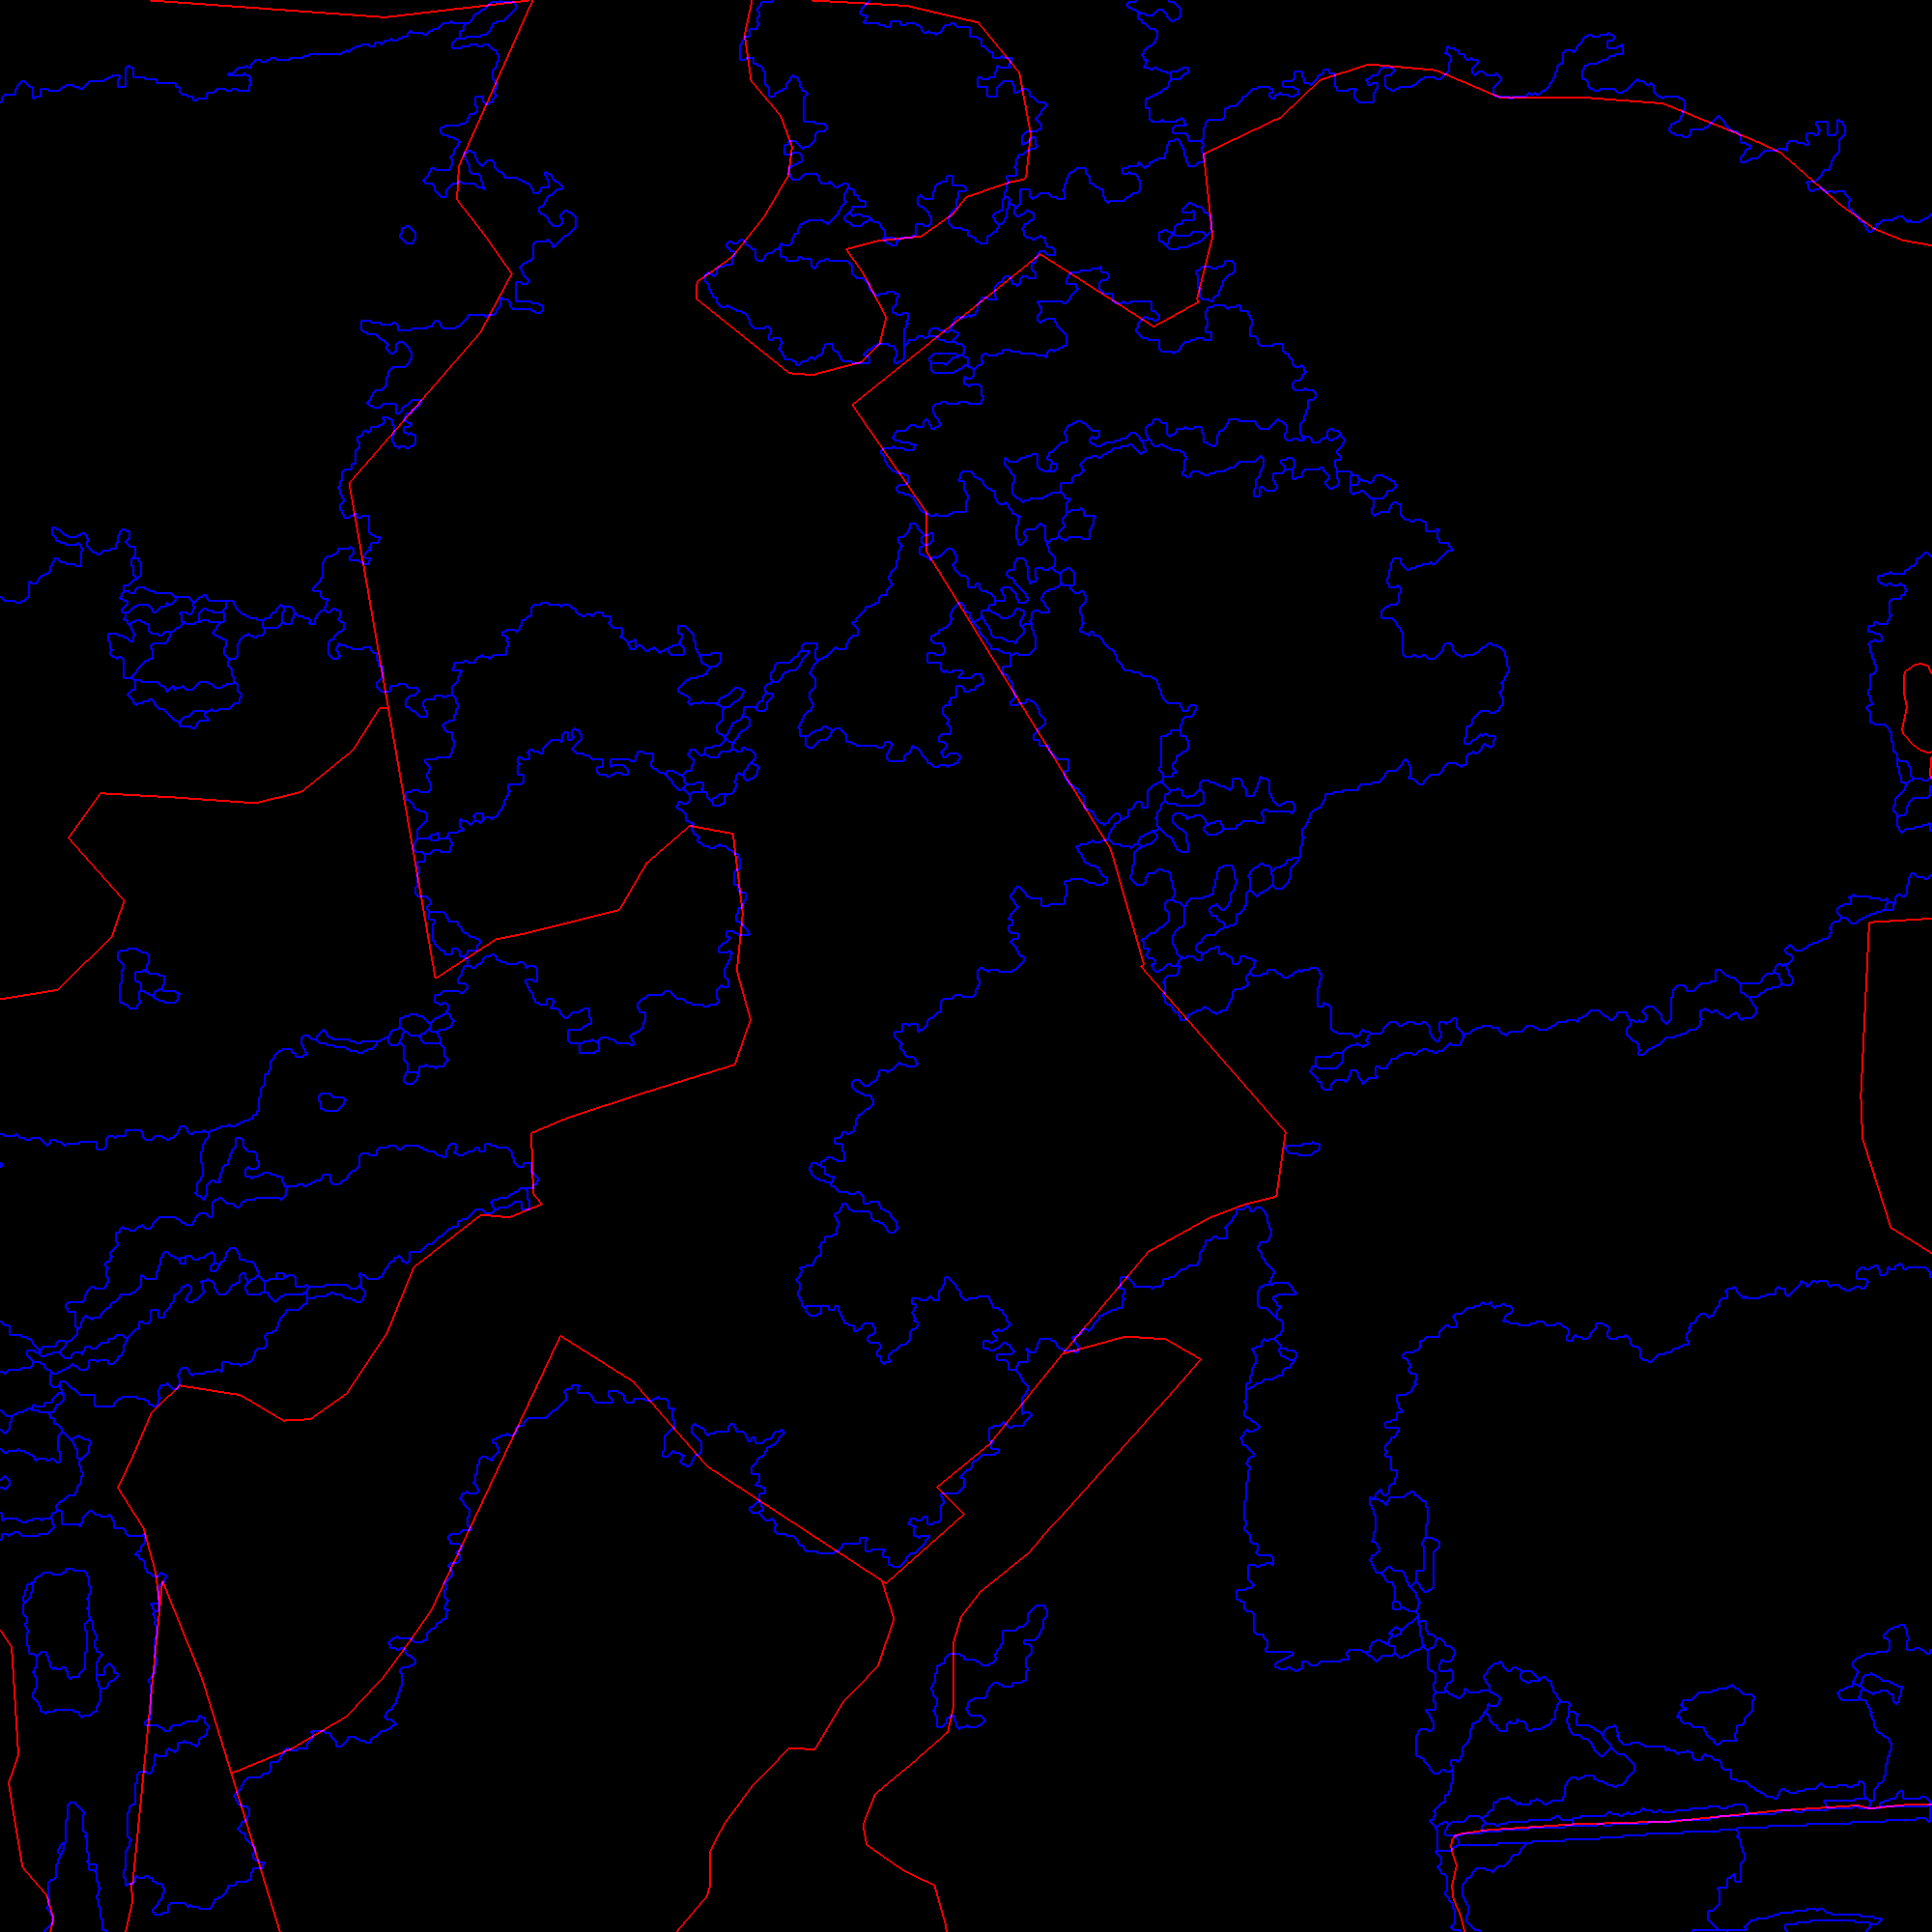
\includegraphics[width=0.45\textwidth]{Figures/C3/S2/seg_herarchical_10border_hierarchical}
\label{subfig:hierar10}
}
\\
\subfloat[Hierarchical segmentation with $\mu=12$.]{
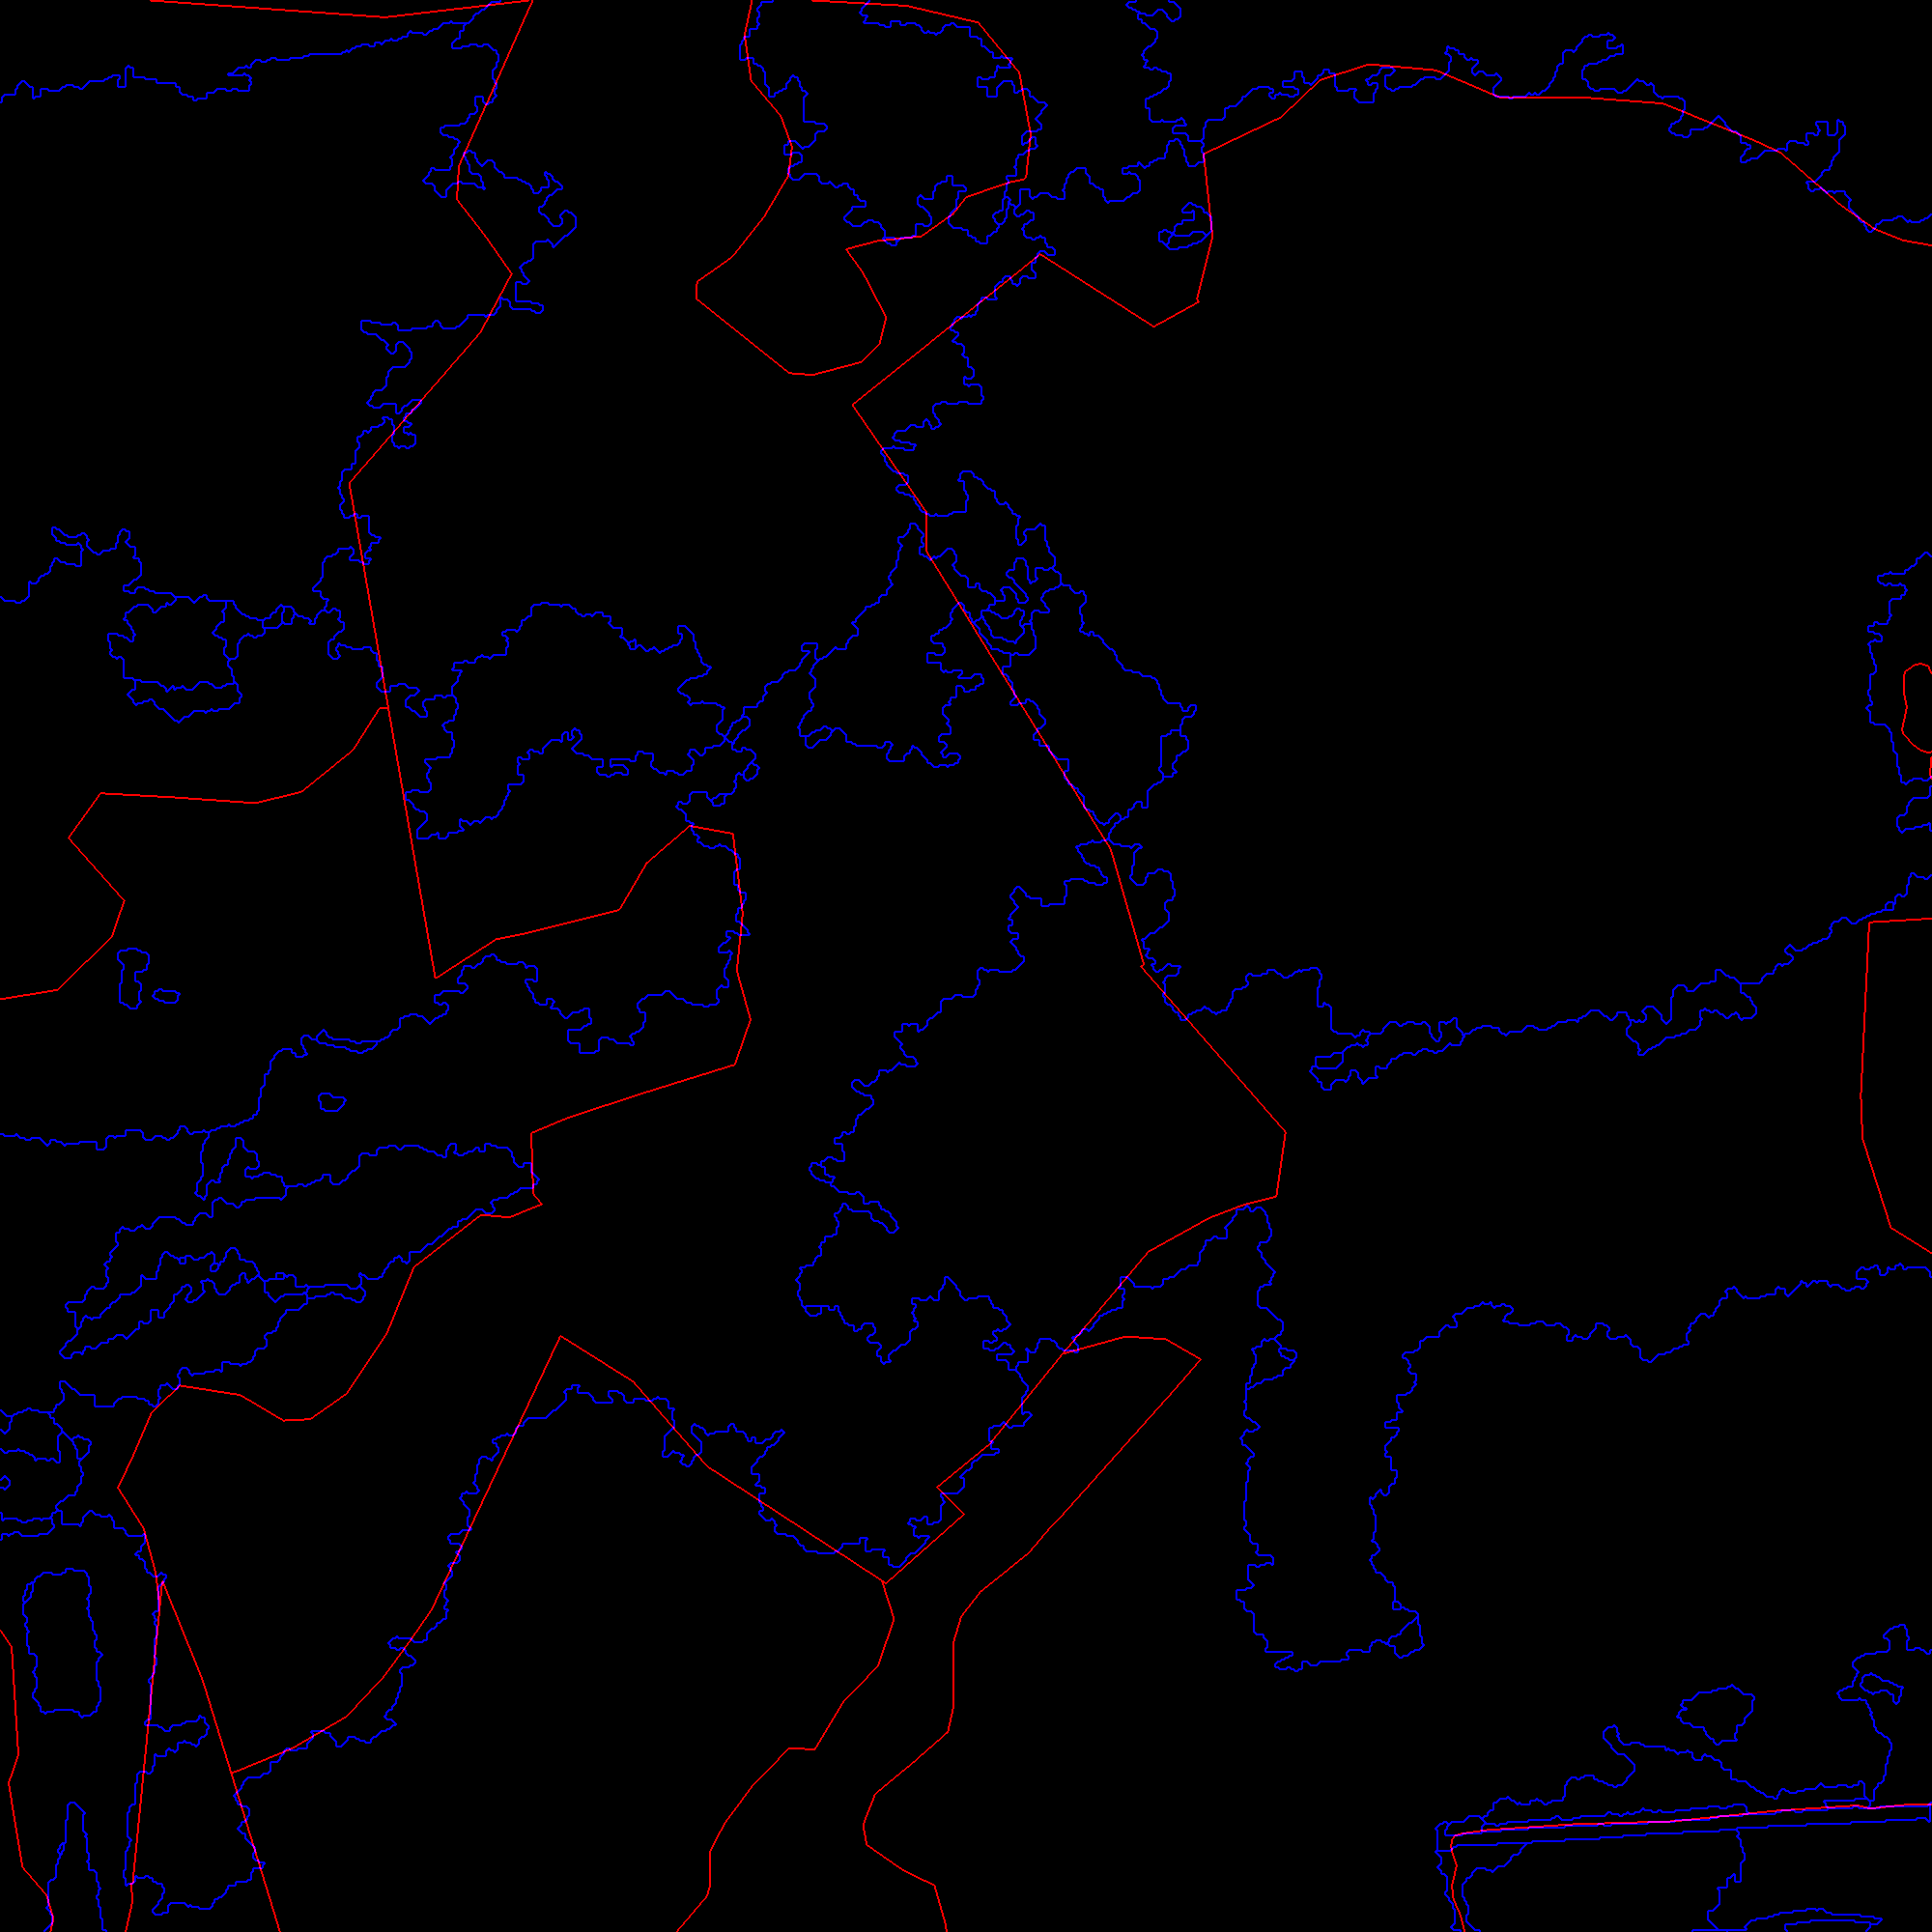
\includegraphics[width=0.45\textwidth]{Figures/C3/S2/seg_herarchical_12border_hierarchical}
\label{subfig:hierar12}
}
\hspace*{0.05\textwidth}
\subfloat[Hierarchical segmentation with $\mu=15$.]{
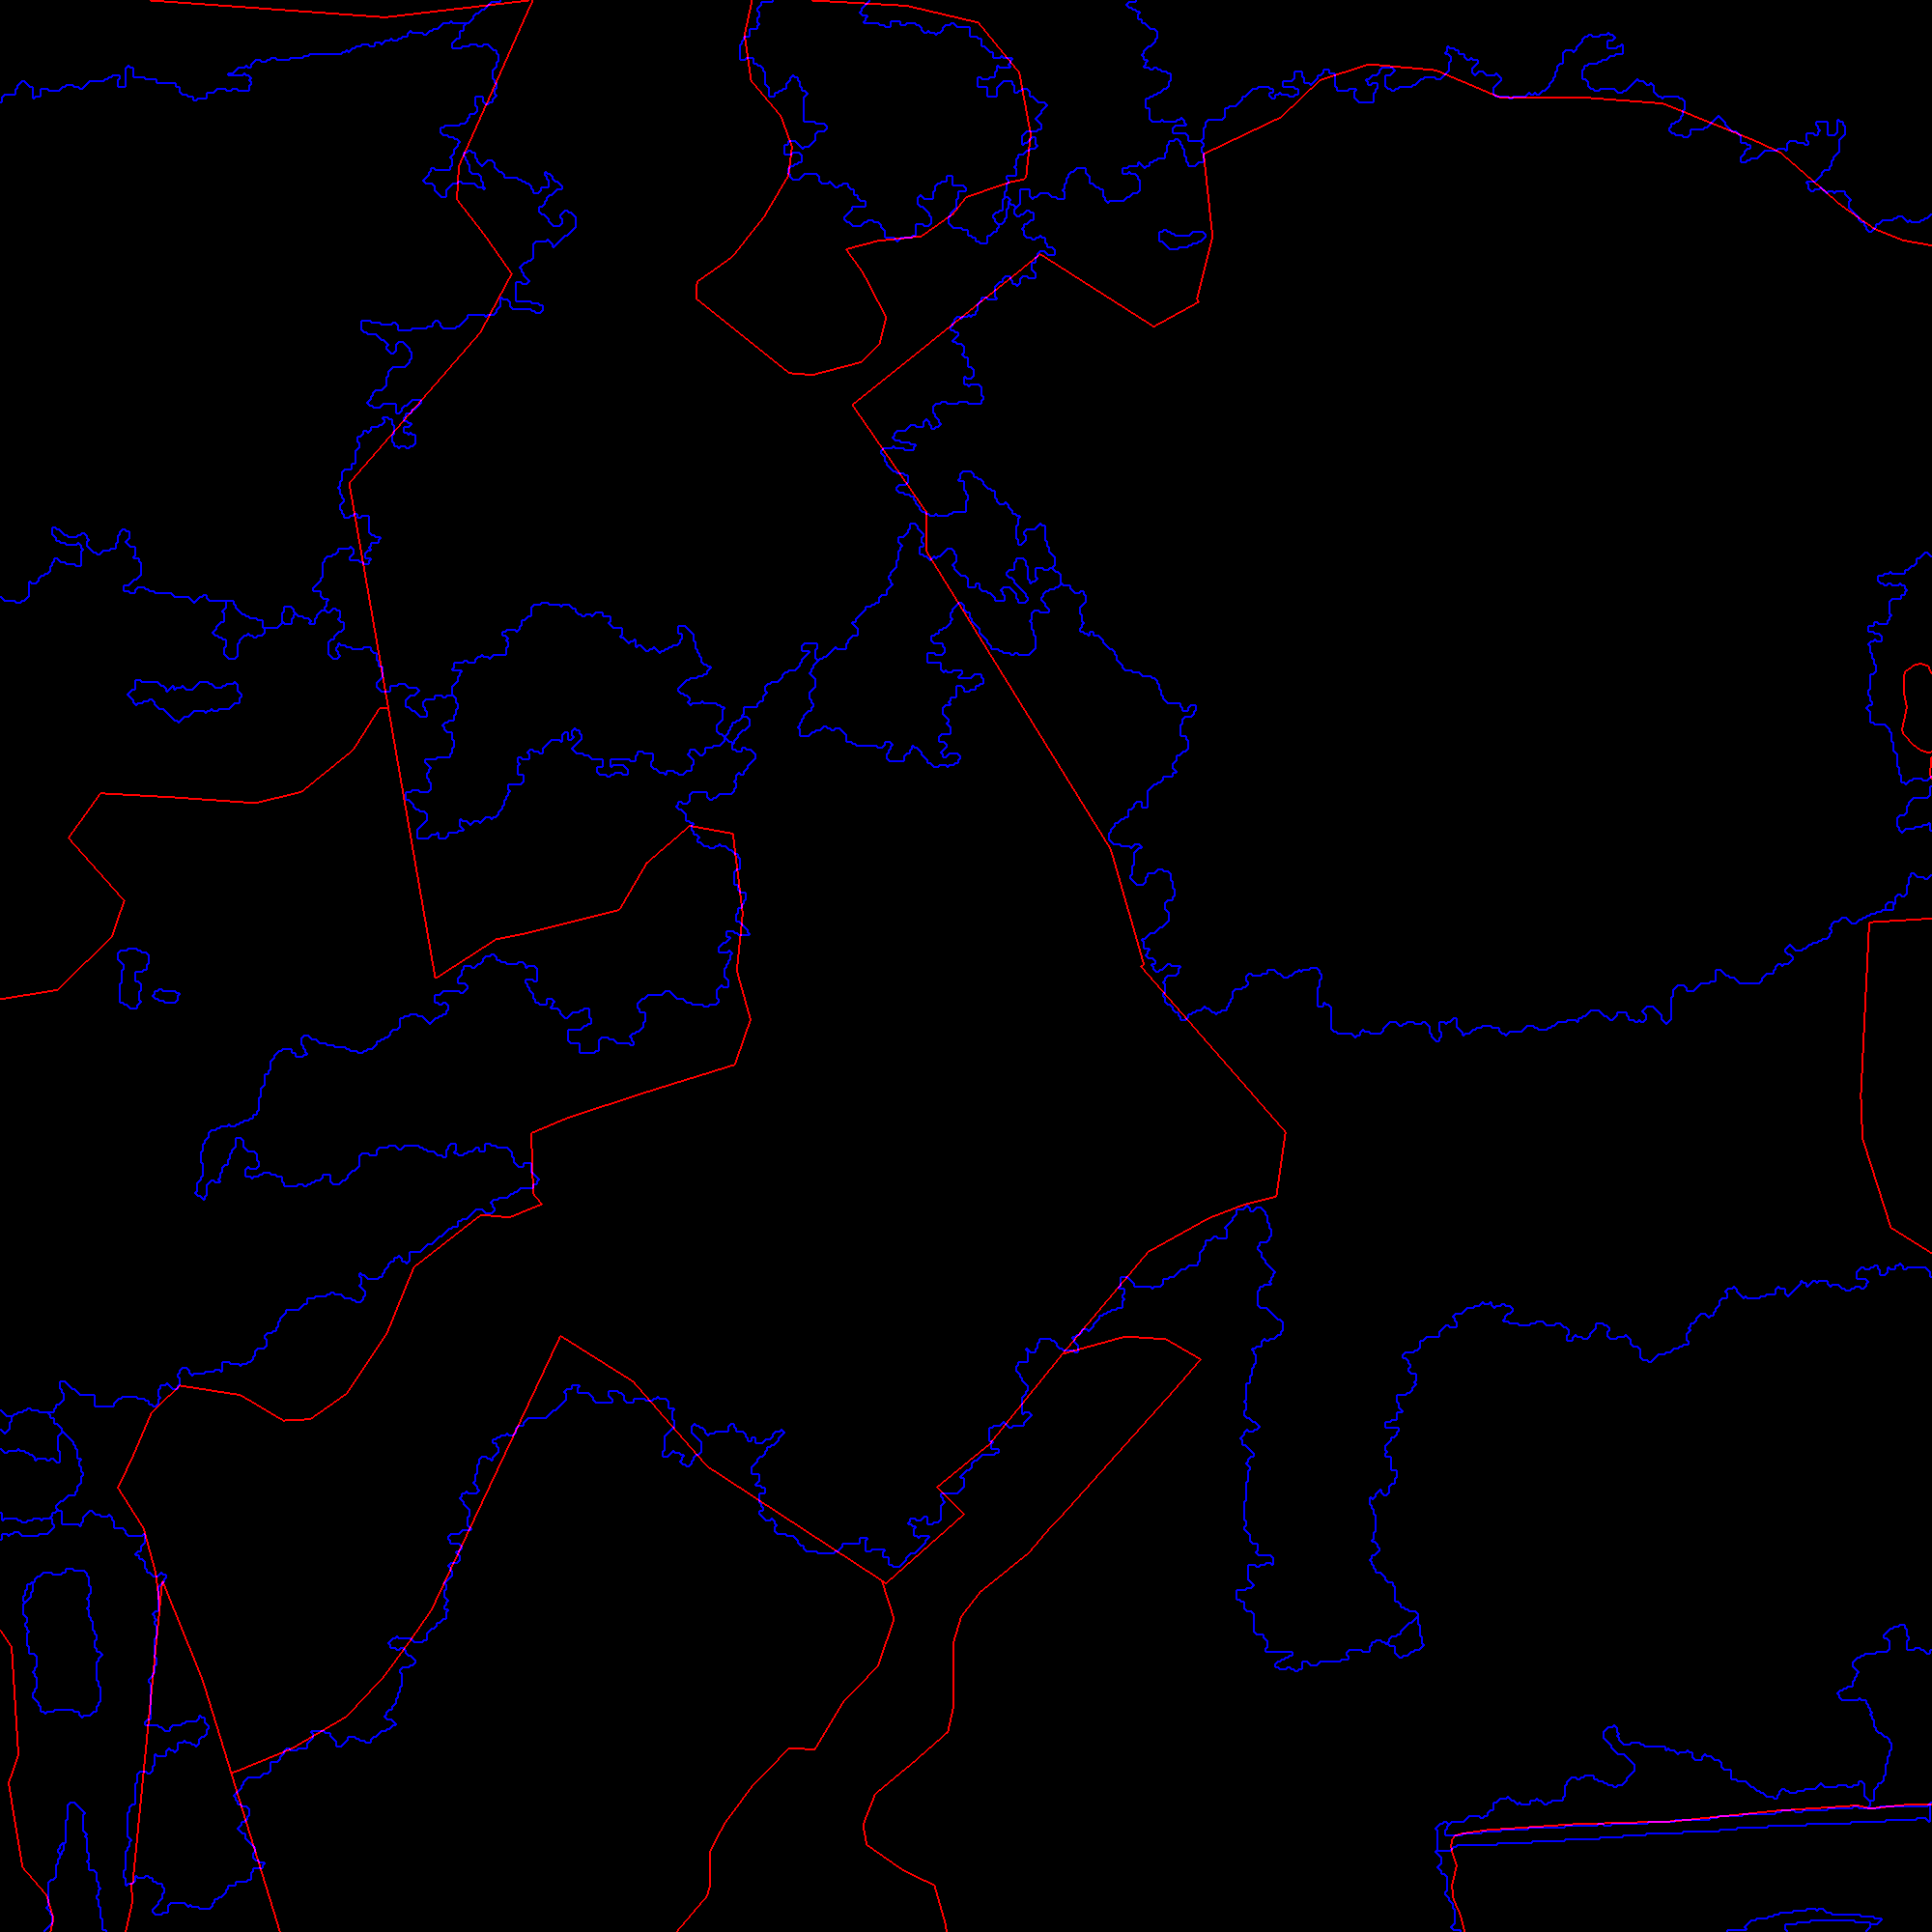
\includegraphics[width=0.45\textwidth]{Figures/C3/S2/seg_herarchical_15border_hierarchical}
\label{subfig:hierar15}
}
\endgroup
\caption{Result of the segmentation of the VHR optical image using different values of $\mu$ for the hierarchical segmentation. Blue lines correspond to the borders of the segments, red lines correspond to the borders of the forest LC.}
\label{fig:hierar}
\end{center}
\end{figure}

The two proposed segmentation algorithms are very efficient for image segmentation tasks \citep{guigues2006scale, felzenszwalb2004efficient} but are not adapted to retrieve forest stands borders. However, they can produce interesting over-segmentation since they are able to retrieve some relevant borders.

\subsection{Add semantic information}
The classification proposed in the method give information about the species at the object level. Since the segments extracted below are large than the small objects, a majority vote can be applied for each segment. The obtained label map could be compared with the forest LC.
The result of the classification for the area of interest is presented in Figure~\ref{fig:C3_S2_classif}, the confusion matrix and other accuracy metrics for this classification are presented in Table~\ref{table:C3_S2_classif}.

\begin{figure}[htbp]
\begin{center}
\begingroup
\captionsetup[subfigure]{width=0.375\textwidth}
\subfloat[Forest LC.]{
\includegraphics[width=0.45\textwidth]{Figures/C3/S2/BD}
\label{subfig:C3_S2_classifa}
}
\hspace*{0.05\textwidth}
\subfloat[Classification results (overall accuracy: 81.75\%, $\kappa$: 0.67).]{
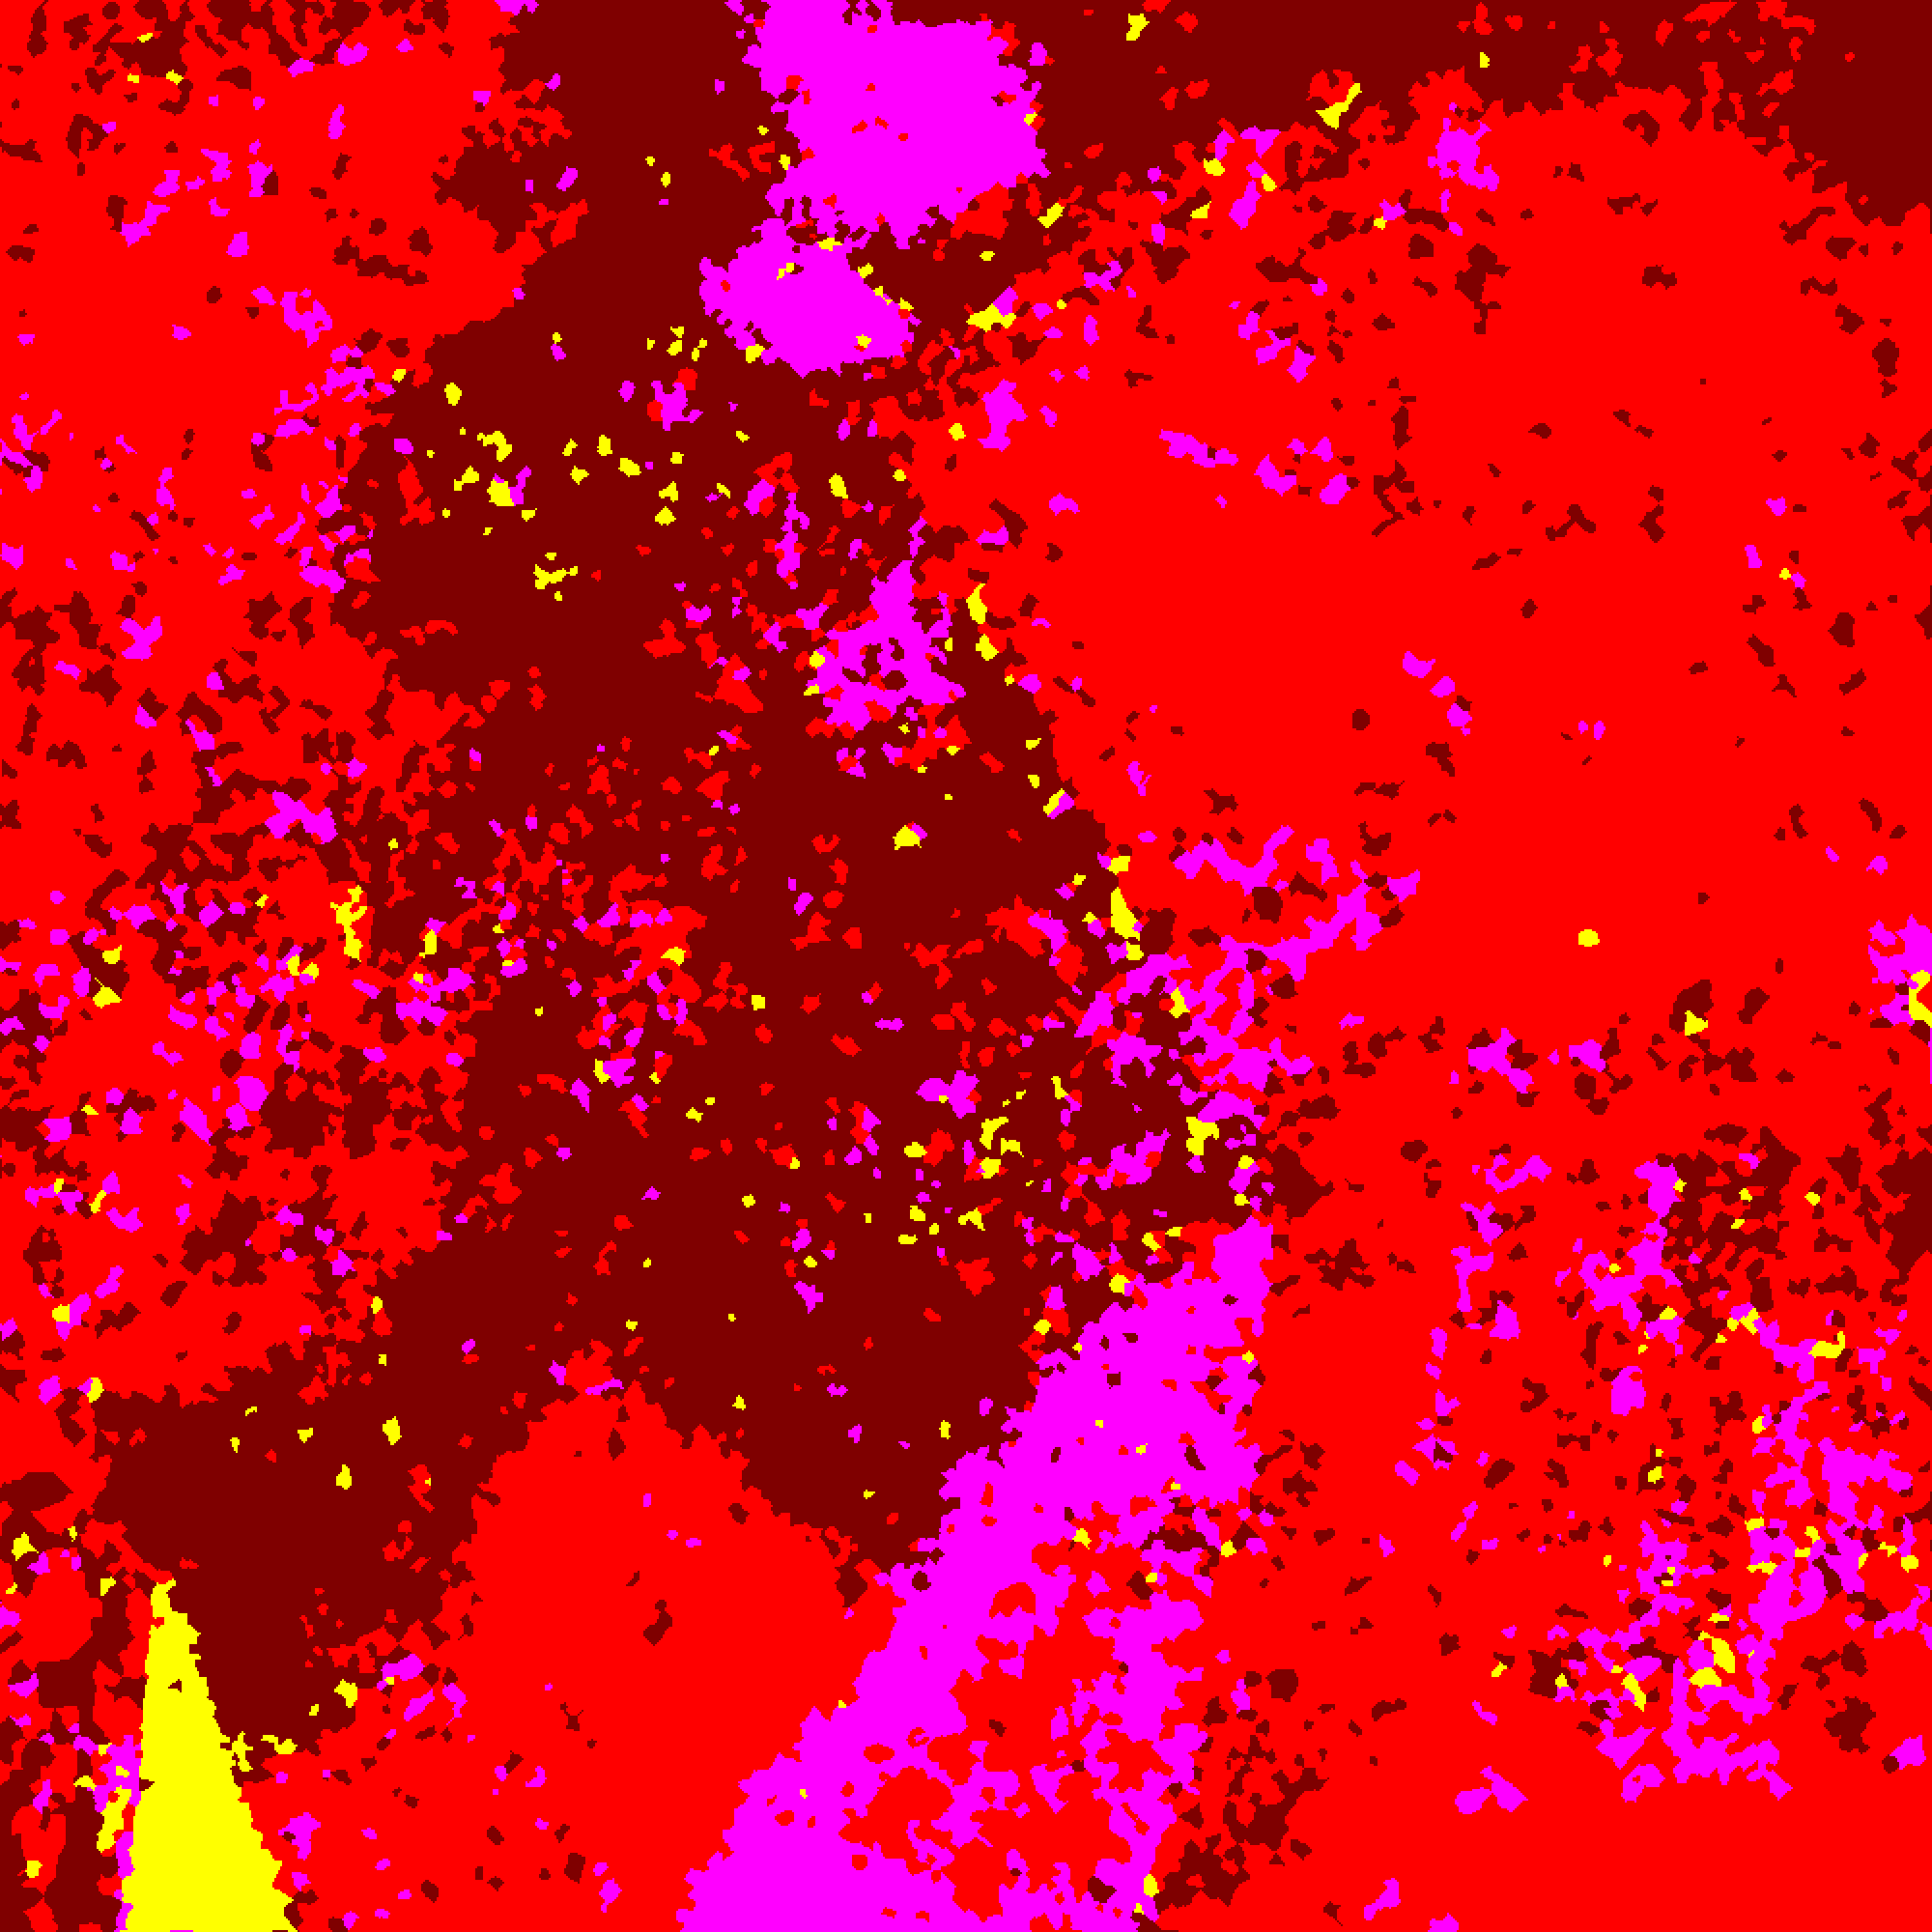
\includegraphics[width=0.45\textwidth]{Figures/C3/S2/classif}
\label{subfig:C3_S2_classifb}
}
\endgroup
\caption{Forest LC and classification results.}
\label{fig:C3_S2_classif}
\end{center}
\end{figure}

The results of the majority vote for the segmentation of the VHR optical images is presented in Figure~\ref{fig:seg_im_sem}, the confusion matrices and other metrics are presented in Tables~\ref{table:C3_S2_seg_hierar} \& \ref{table:C3_S2_seg_PFF}.

\begin{figure}[htbp]
\begin{center}
\begingroup
\captionsetup[subfigure]{width=0.3\textwidth}
\subfloat[Forest LC database.]{
\includegraphics[width=0.3\textwidth]{Figures/C3/S2/BD}
\label{subfig:seg_im_sema}
}
\hspace*{0.025\textwidth}
\subfloat[Semantic information for the hierarchical segmentation with $\mu=15$.]{
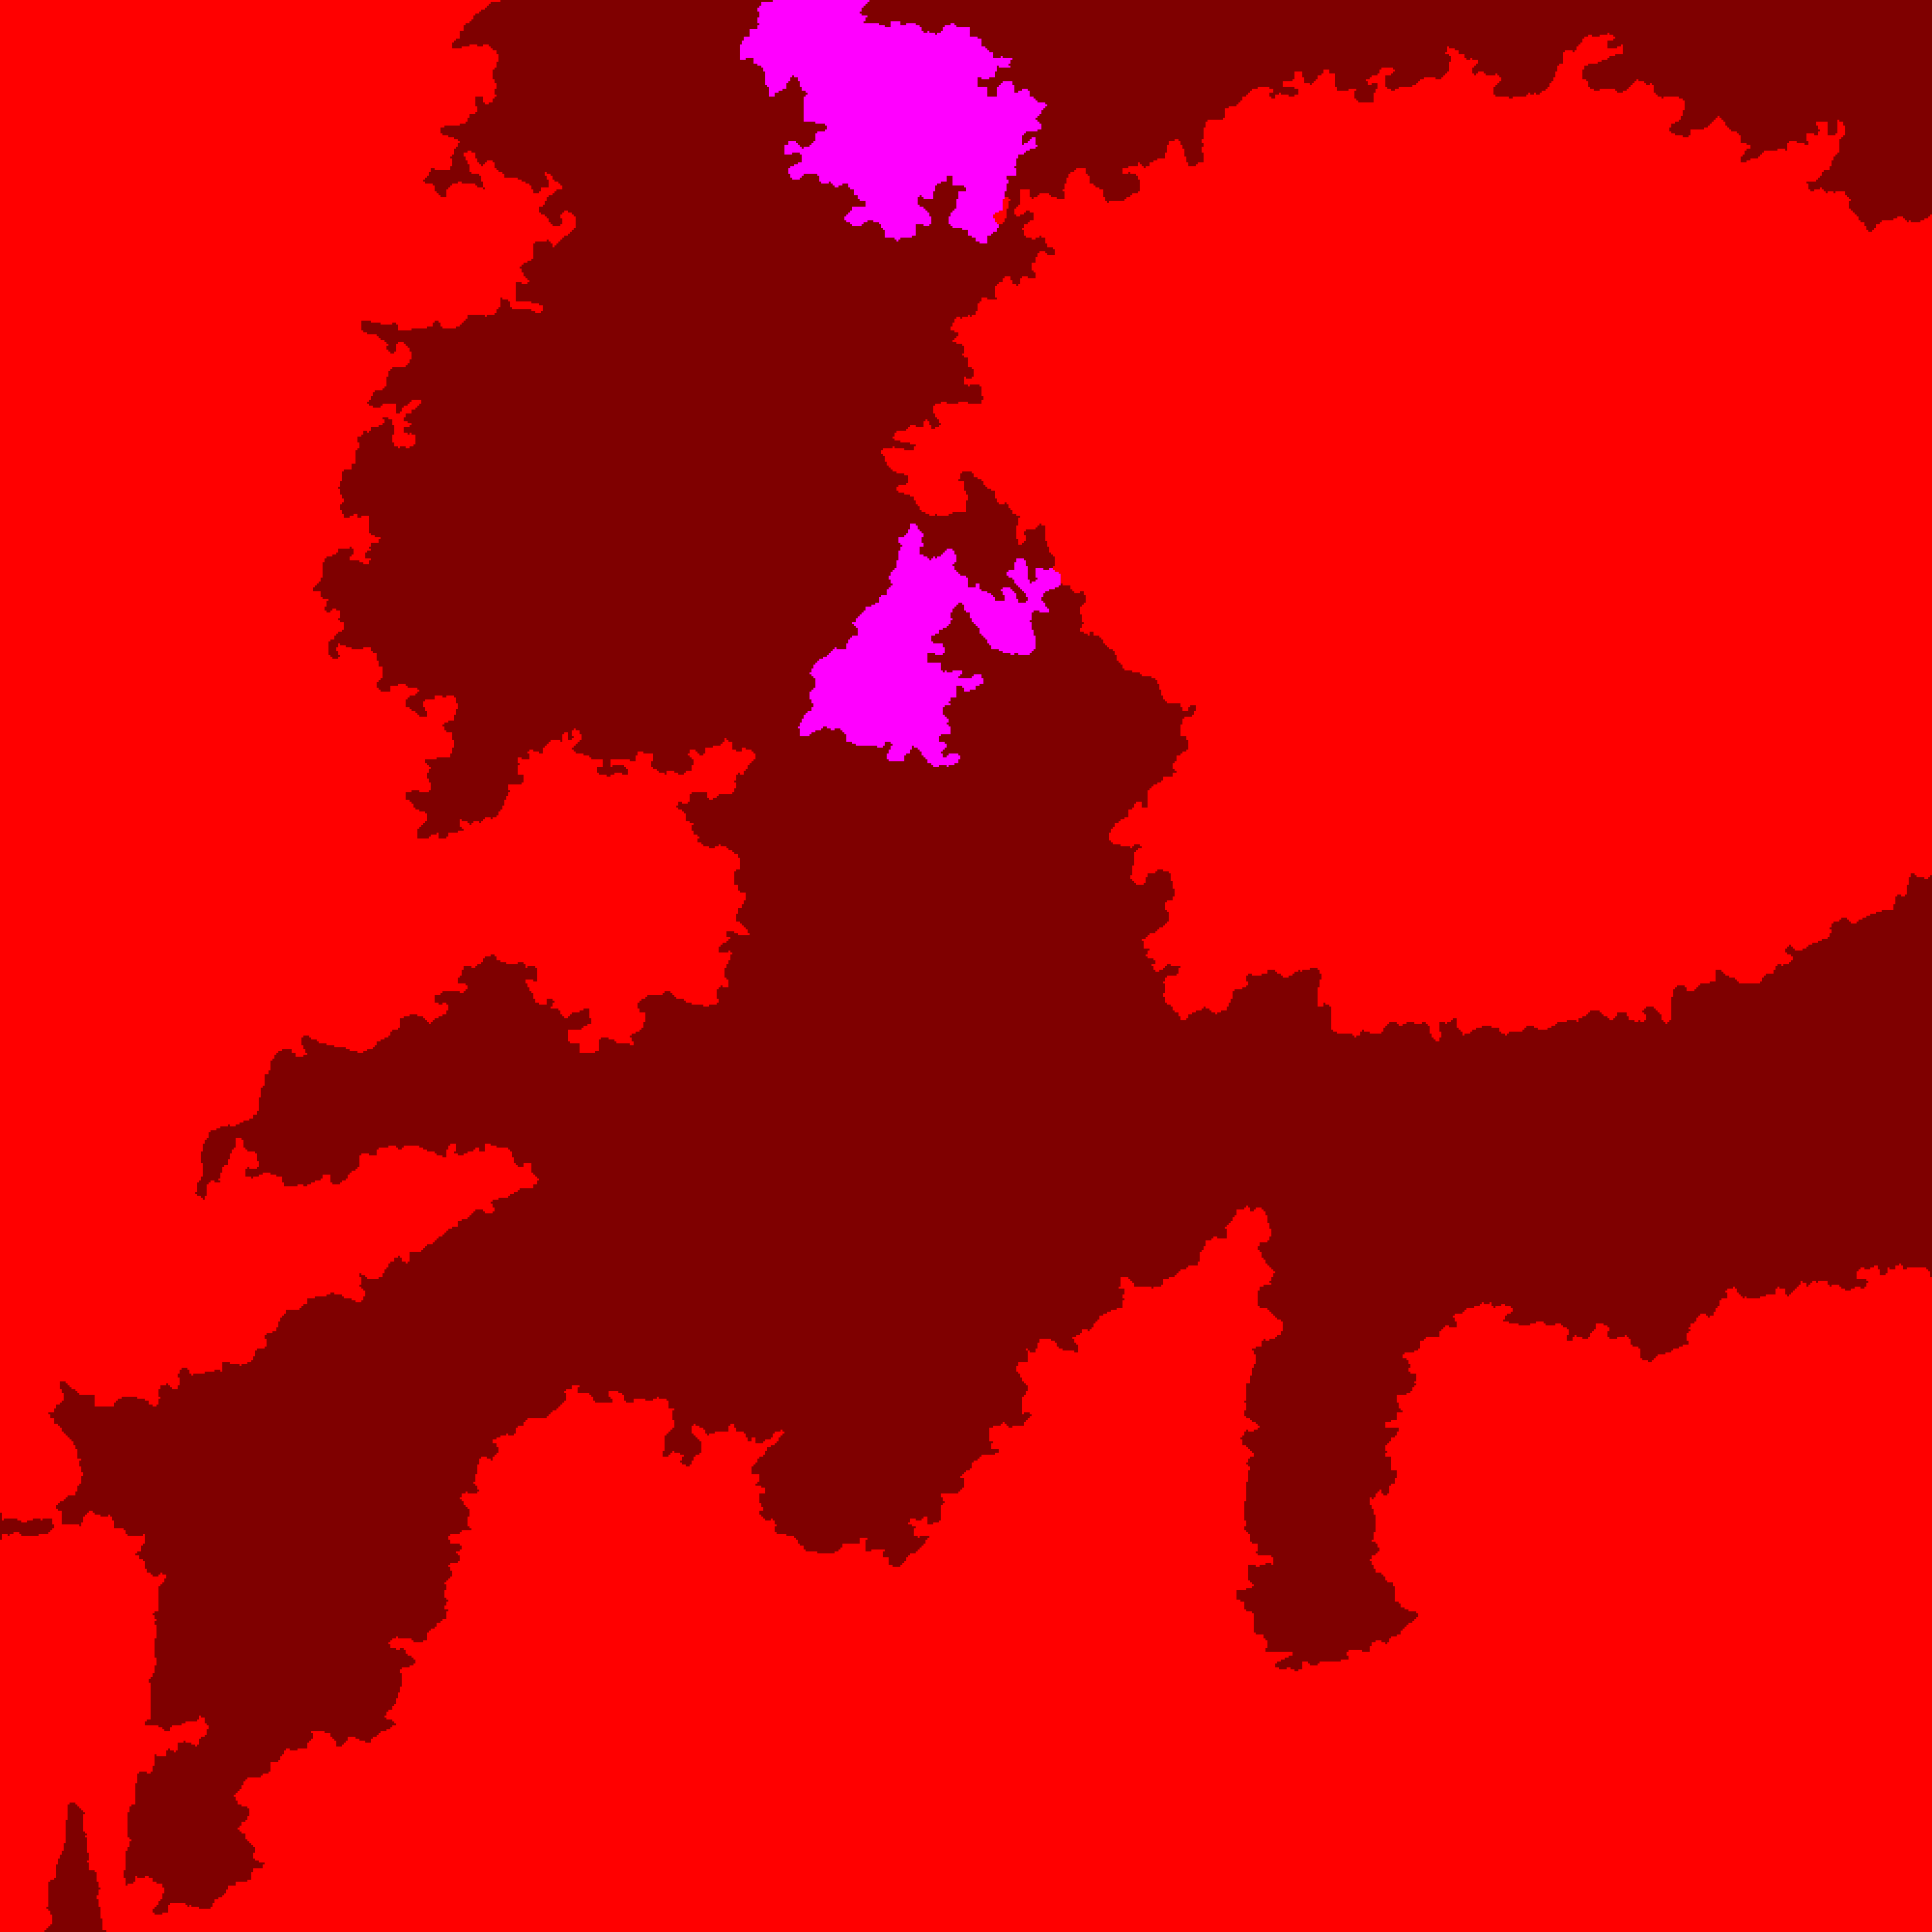
\includegraphics[width=0.3\textwidth]{Figures/C3/S2/seg_hierar_colored}
\label{subfig:seg_im_semb}
}
\hspace*{0.025\textwidth}
\subfloat[Semantic information for the PFF segmentation with $\sigma=0.8$, $k=500$ and $m=40000$.]{
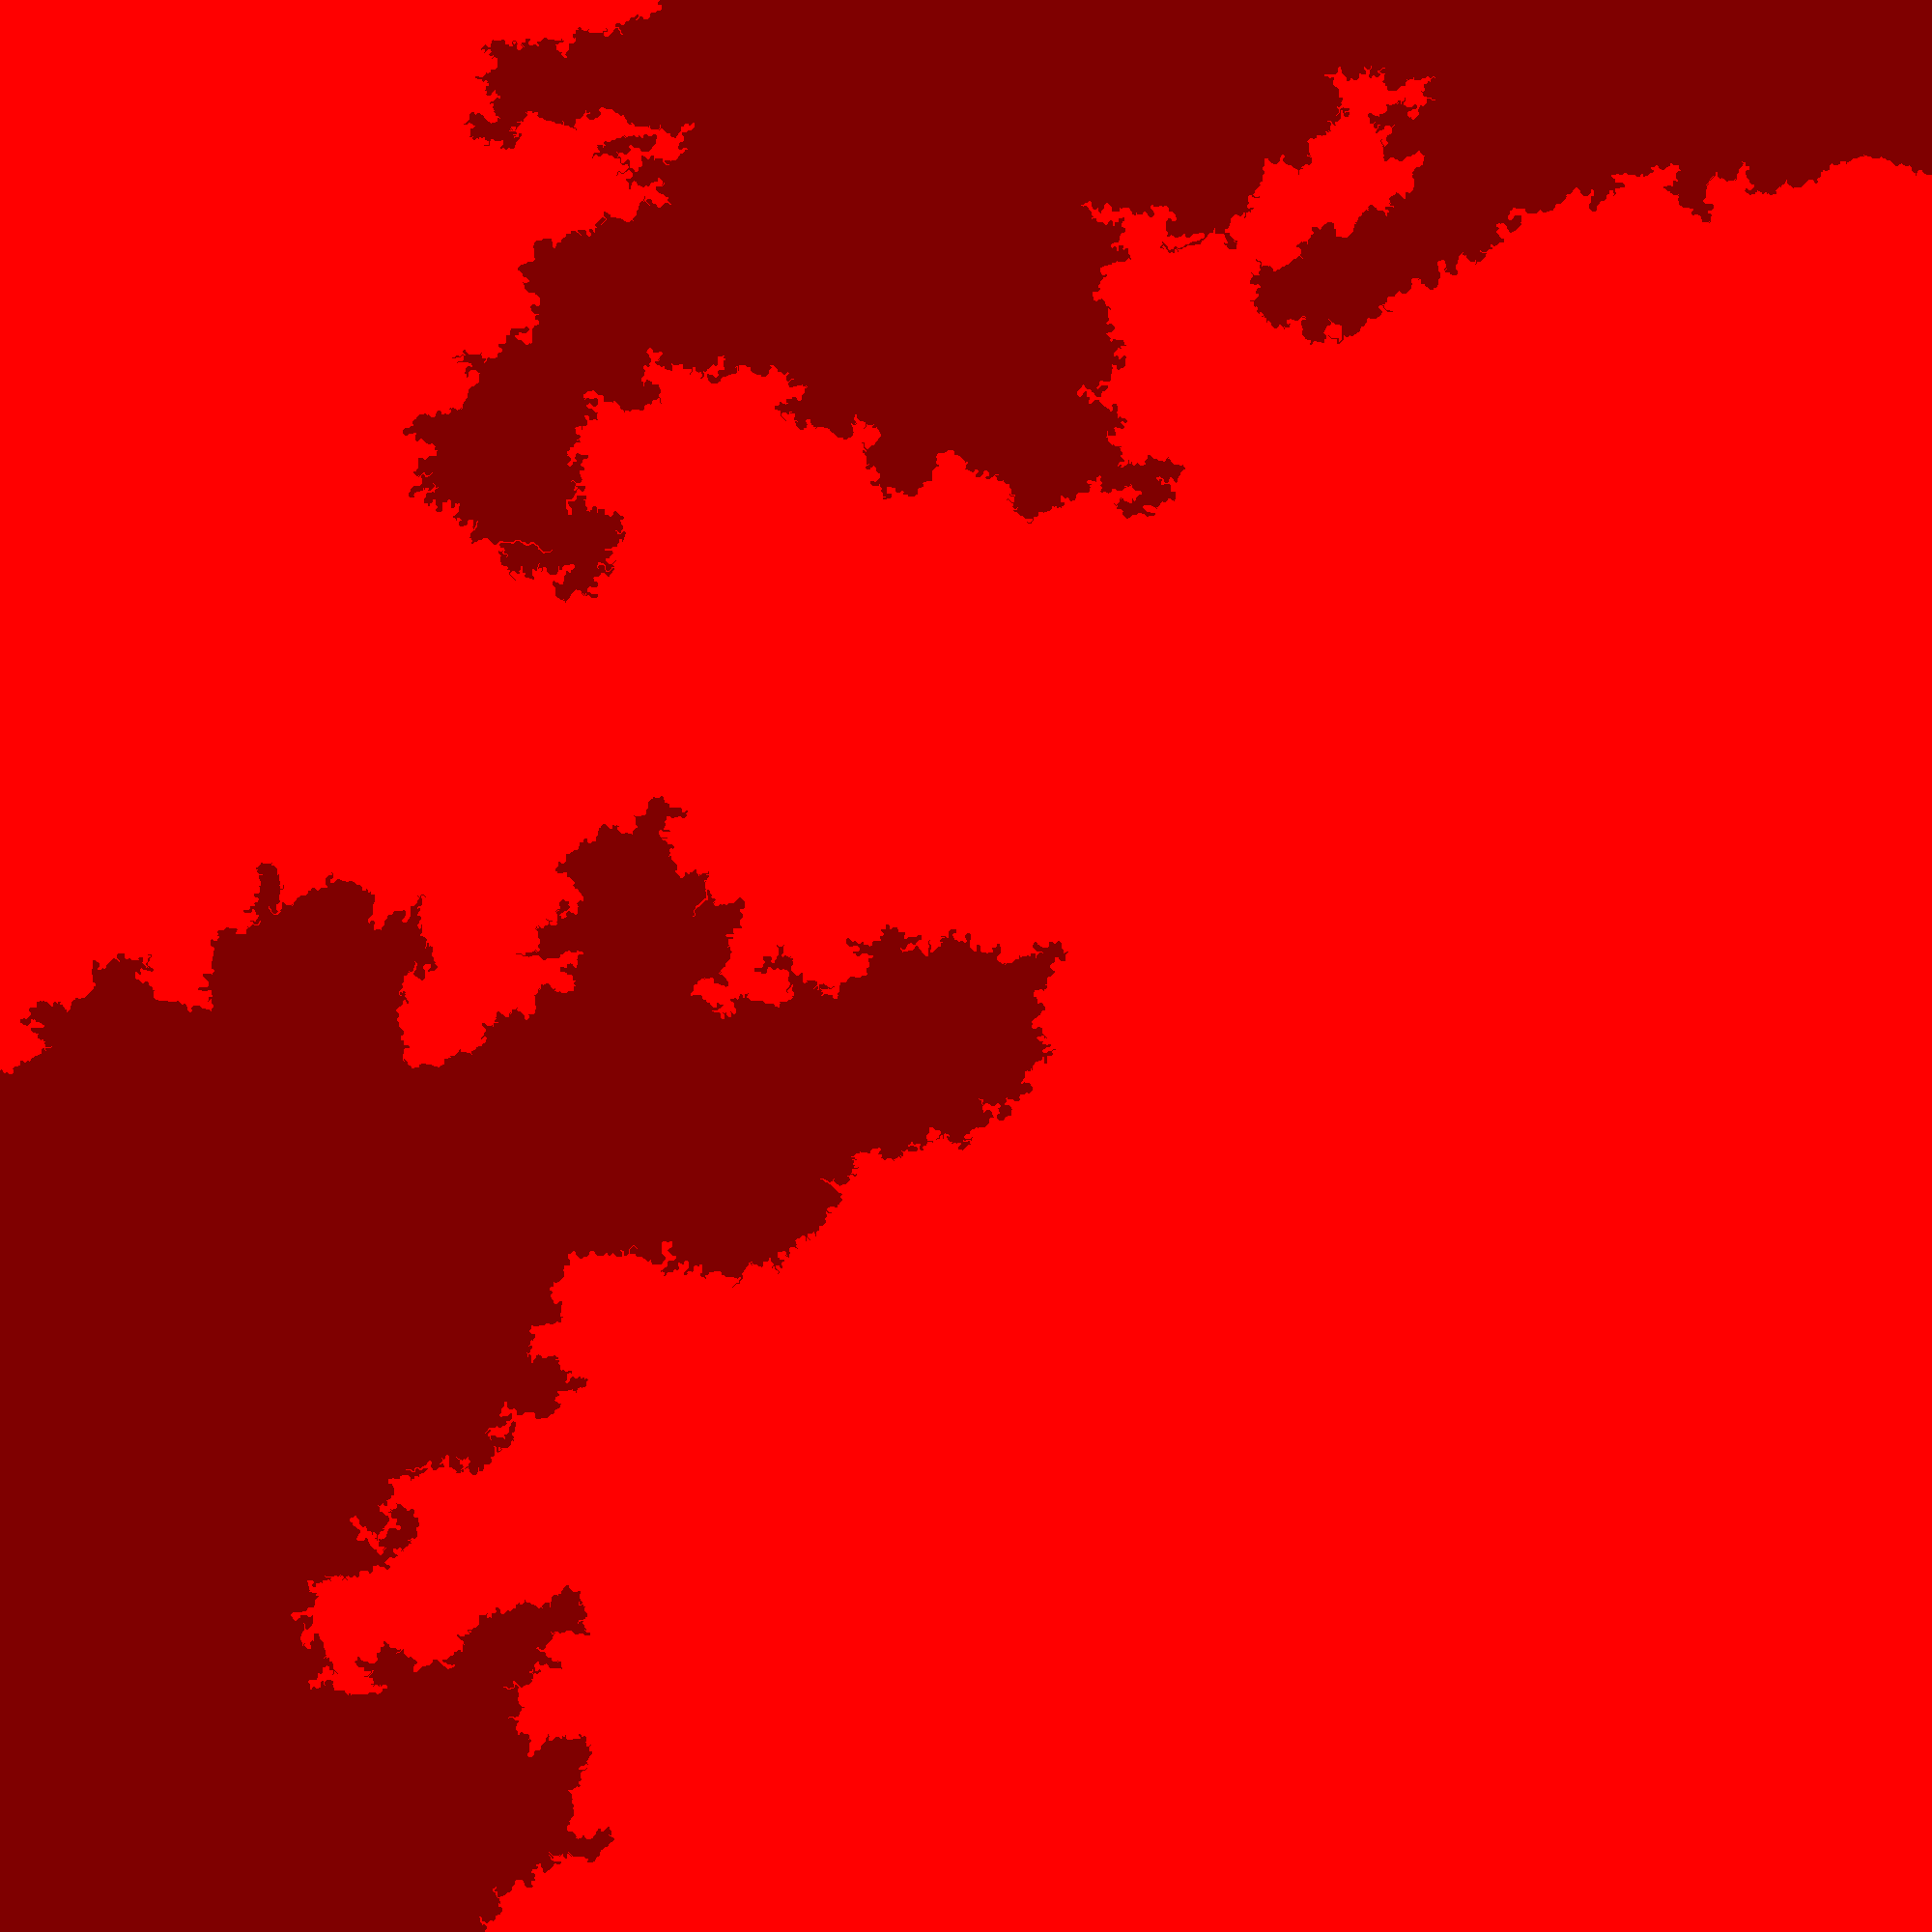
\includegraphics[width=0.3\textwidth]{Figures/C3/S2/seg_PFF_colored}
\label{subfig:seg_im_semc}
}
\endgroup
\caption{Results of the majority vote on the segmentation of the VHR optical images.}
\label{fig:seg_im_sem}
\end{center}
\end{figure}

From a visual inspection, it appears that adding semantic information to the obtained segments does not allow to retrieve a relevant mapping. Indeed, some classes are not represented. For the hierarchical segmentation, the overall accuracy increases when adding semantic information through majority vote (81.94\%, versus 81.75\% for the classification). The $\kappa$ (0.64) is also revealing a good agreement. This shows the limitation of the two metrics: the result appears to be good when inspecting them, while it is not. The Intersection over Union is more relevant in order to underline the irrelevance of the majority vote on a segmentation (41.1\%). The F-score (50.68\%) also concurs to this conclusion.

The results of the majority vote for the segmentation of the nDSM is presented in Figure~\ref{fig:seg_z_sem}, the confusion matrices and other metrics are presented in Tables~\ref{table:C3_S2_seg_hierar_z} \& \ref{table:C3_S2_seg_PFF_z}.

\begin{figure}[htbp]
\begin{center}
\begingroup
\captionsetup[subfigure]{width=0.3\textwidth}
\subfloat[Forest LC database.]{
\includegraphics[width=0.3\textwidth]{Figures/C3/S2/BD}
\label{subfig:seg_z_sema}
}
\hspace*{0.025\textwidth}
\subfloat[Semantic information for the hierarchical segmentation with $\mu=15$.]{
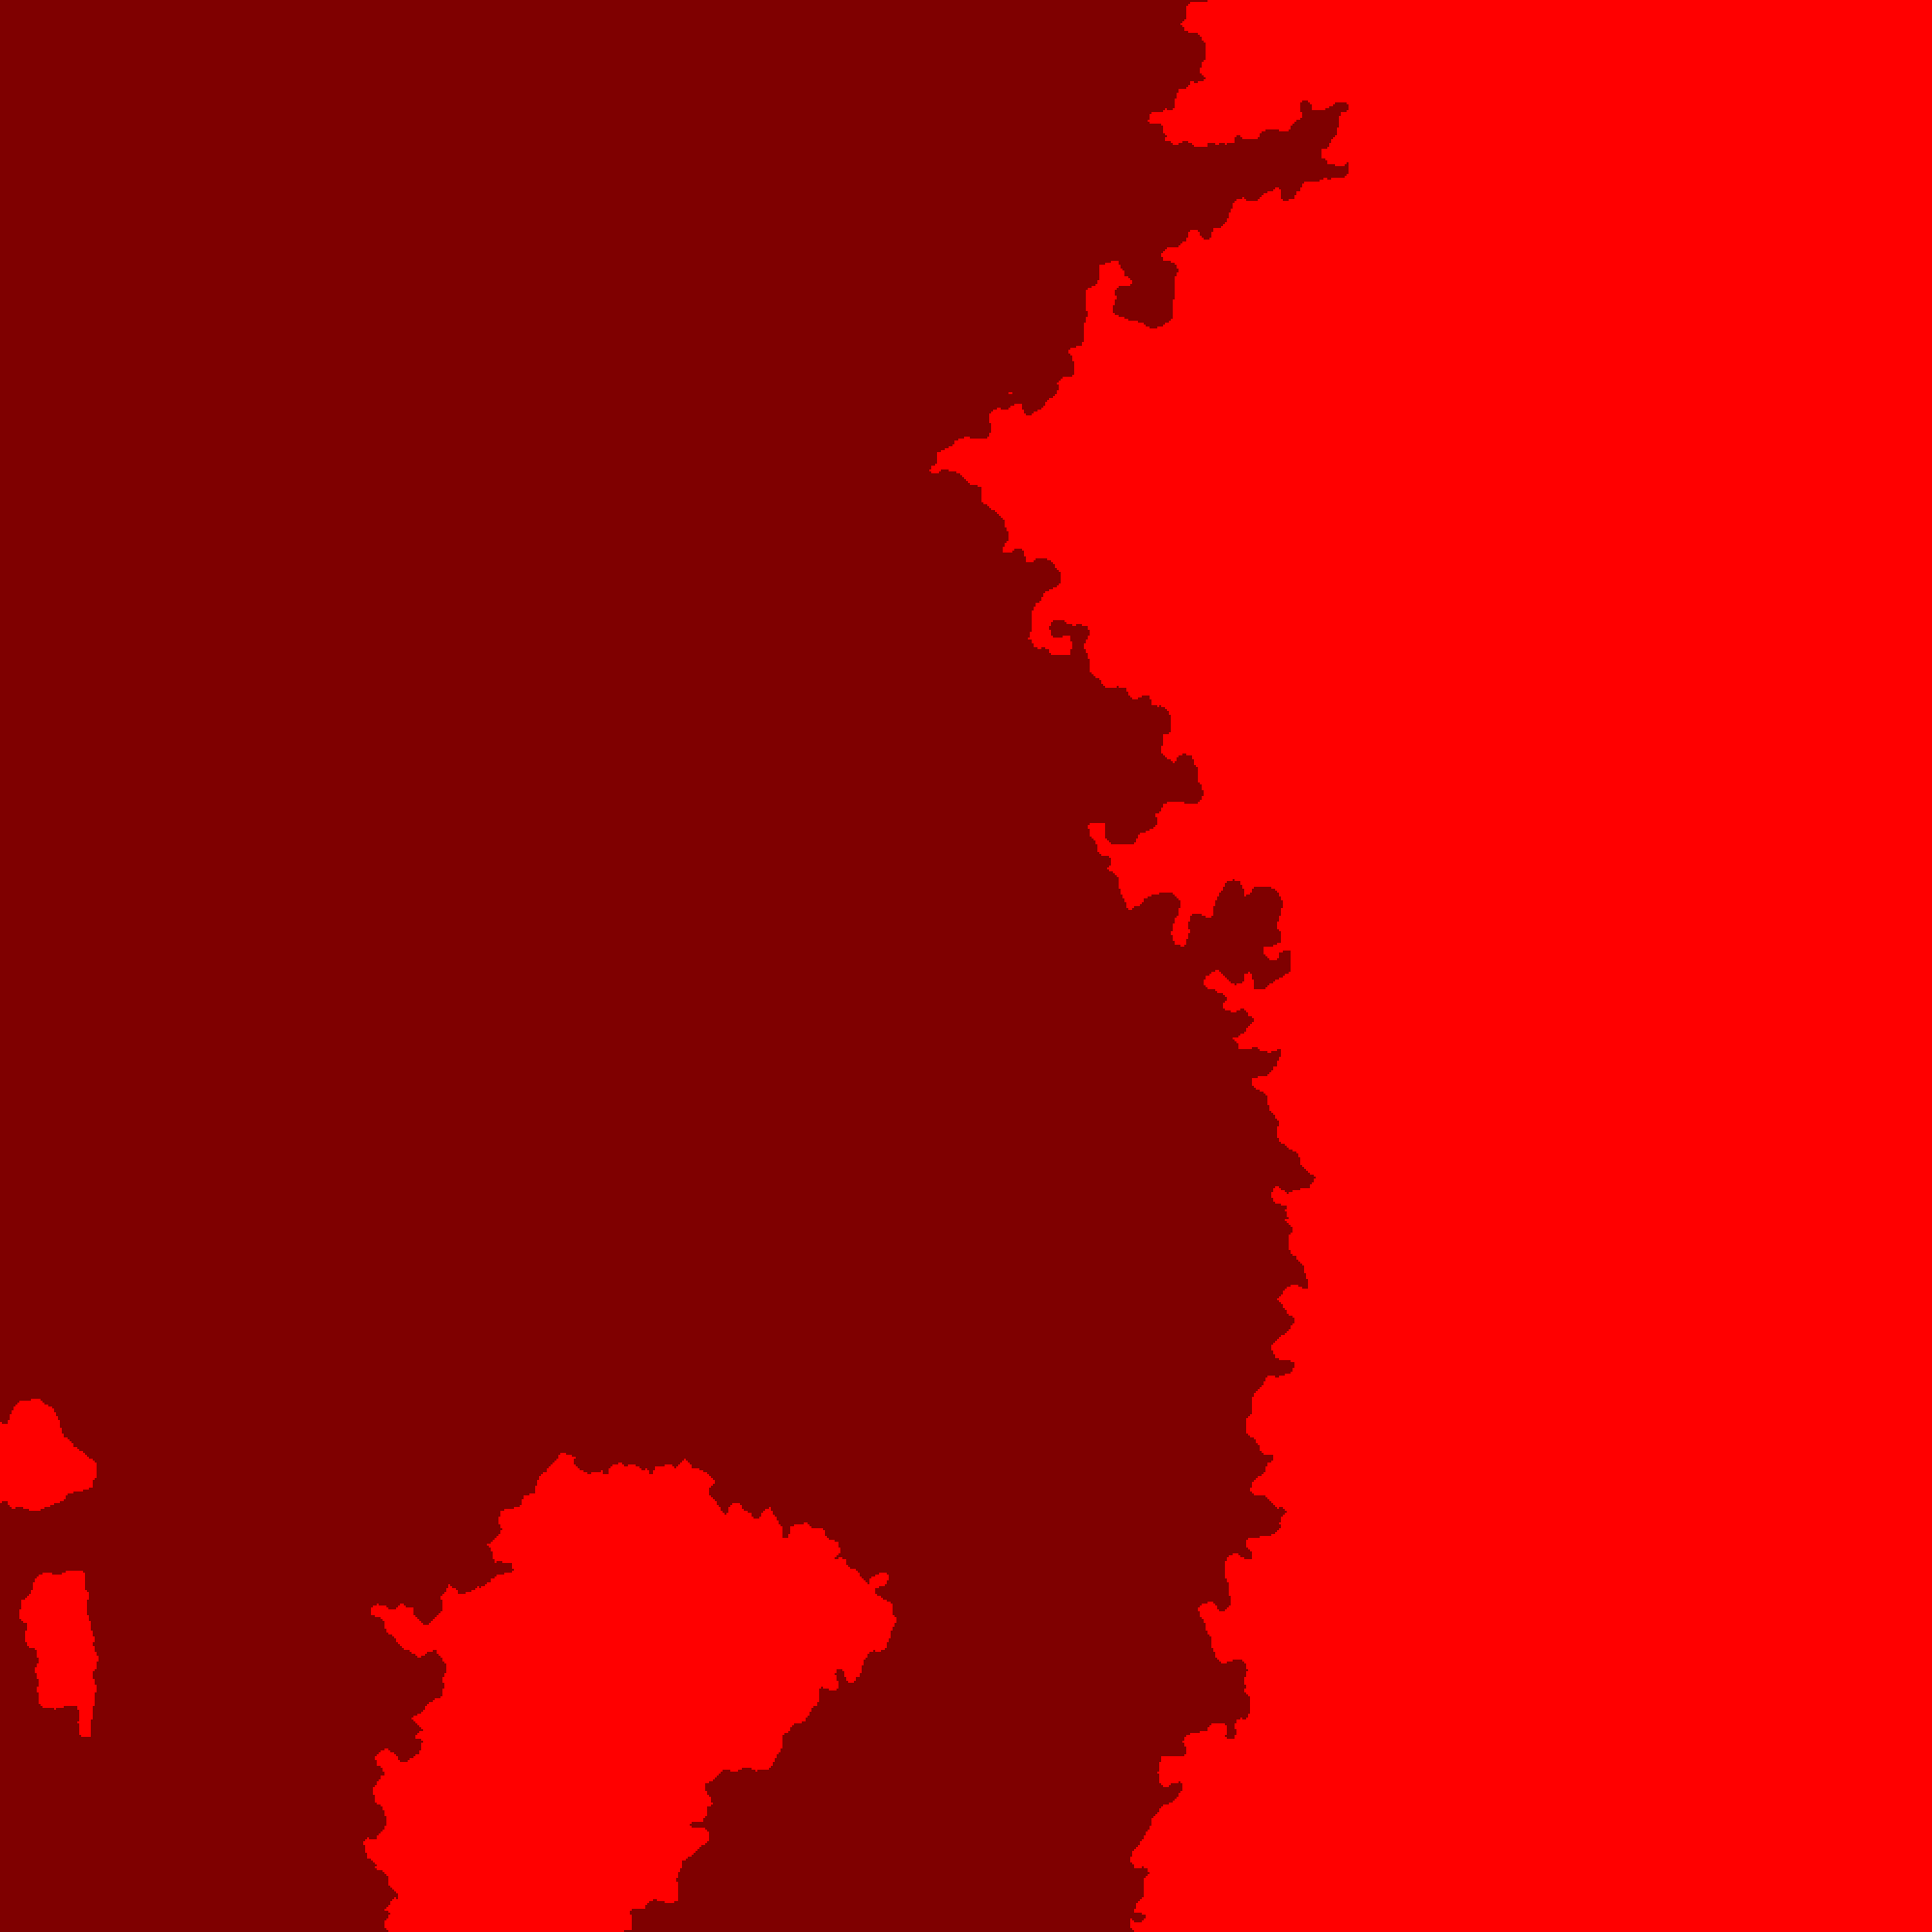
\includegraphics[width=0.3\textwidth]{Figures/C3/S2/seg_hierar_z_colored}
\label{subfig:seg_z_semb}
}
\hspace*{0.025\textwidth}
\subfloat[Semantic information for the PFF segmentation with $\sigma=0.8$, $k=500$ and $m=40000$.]{
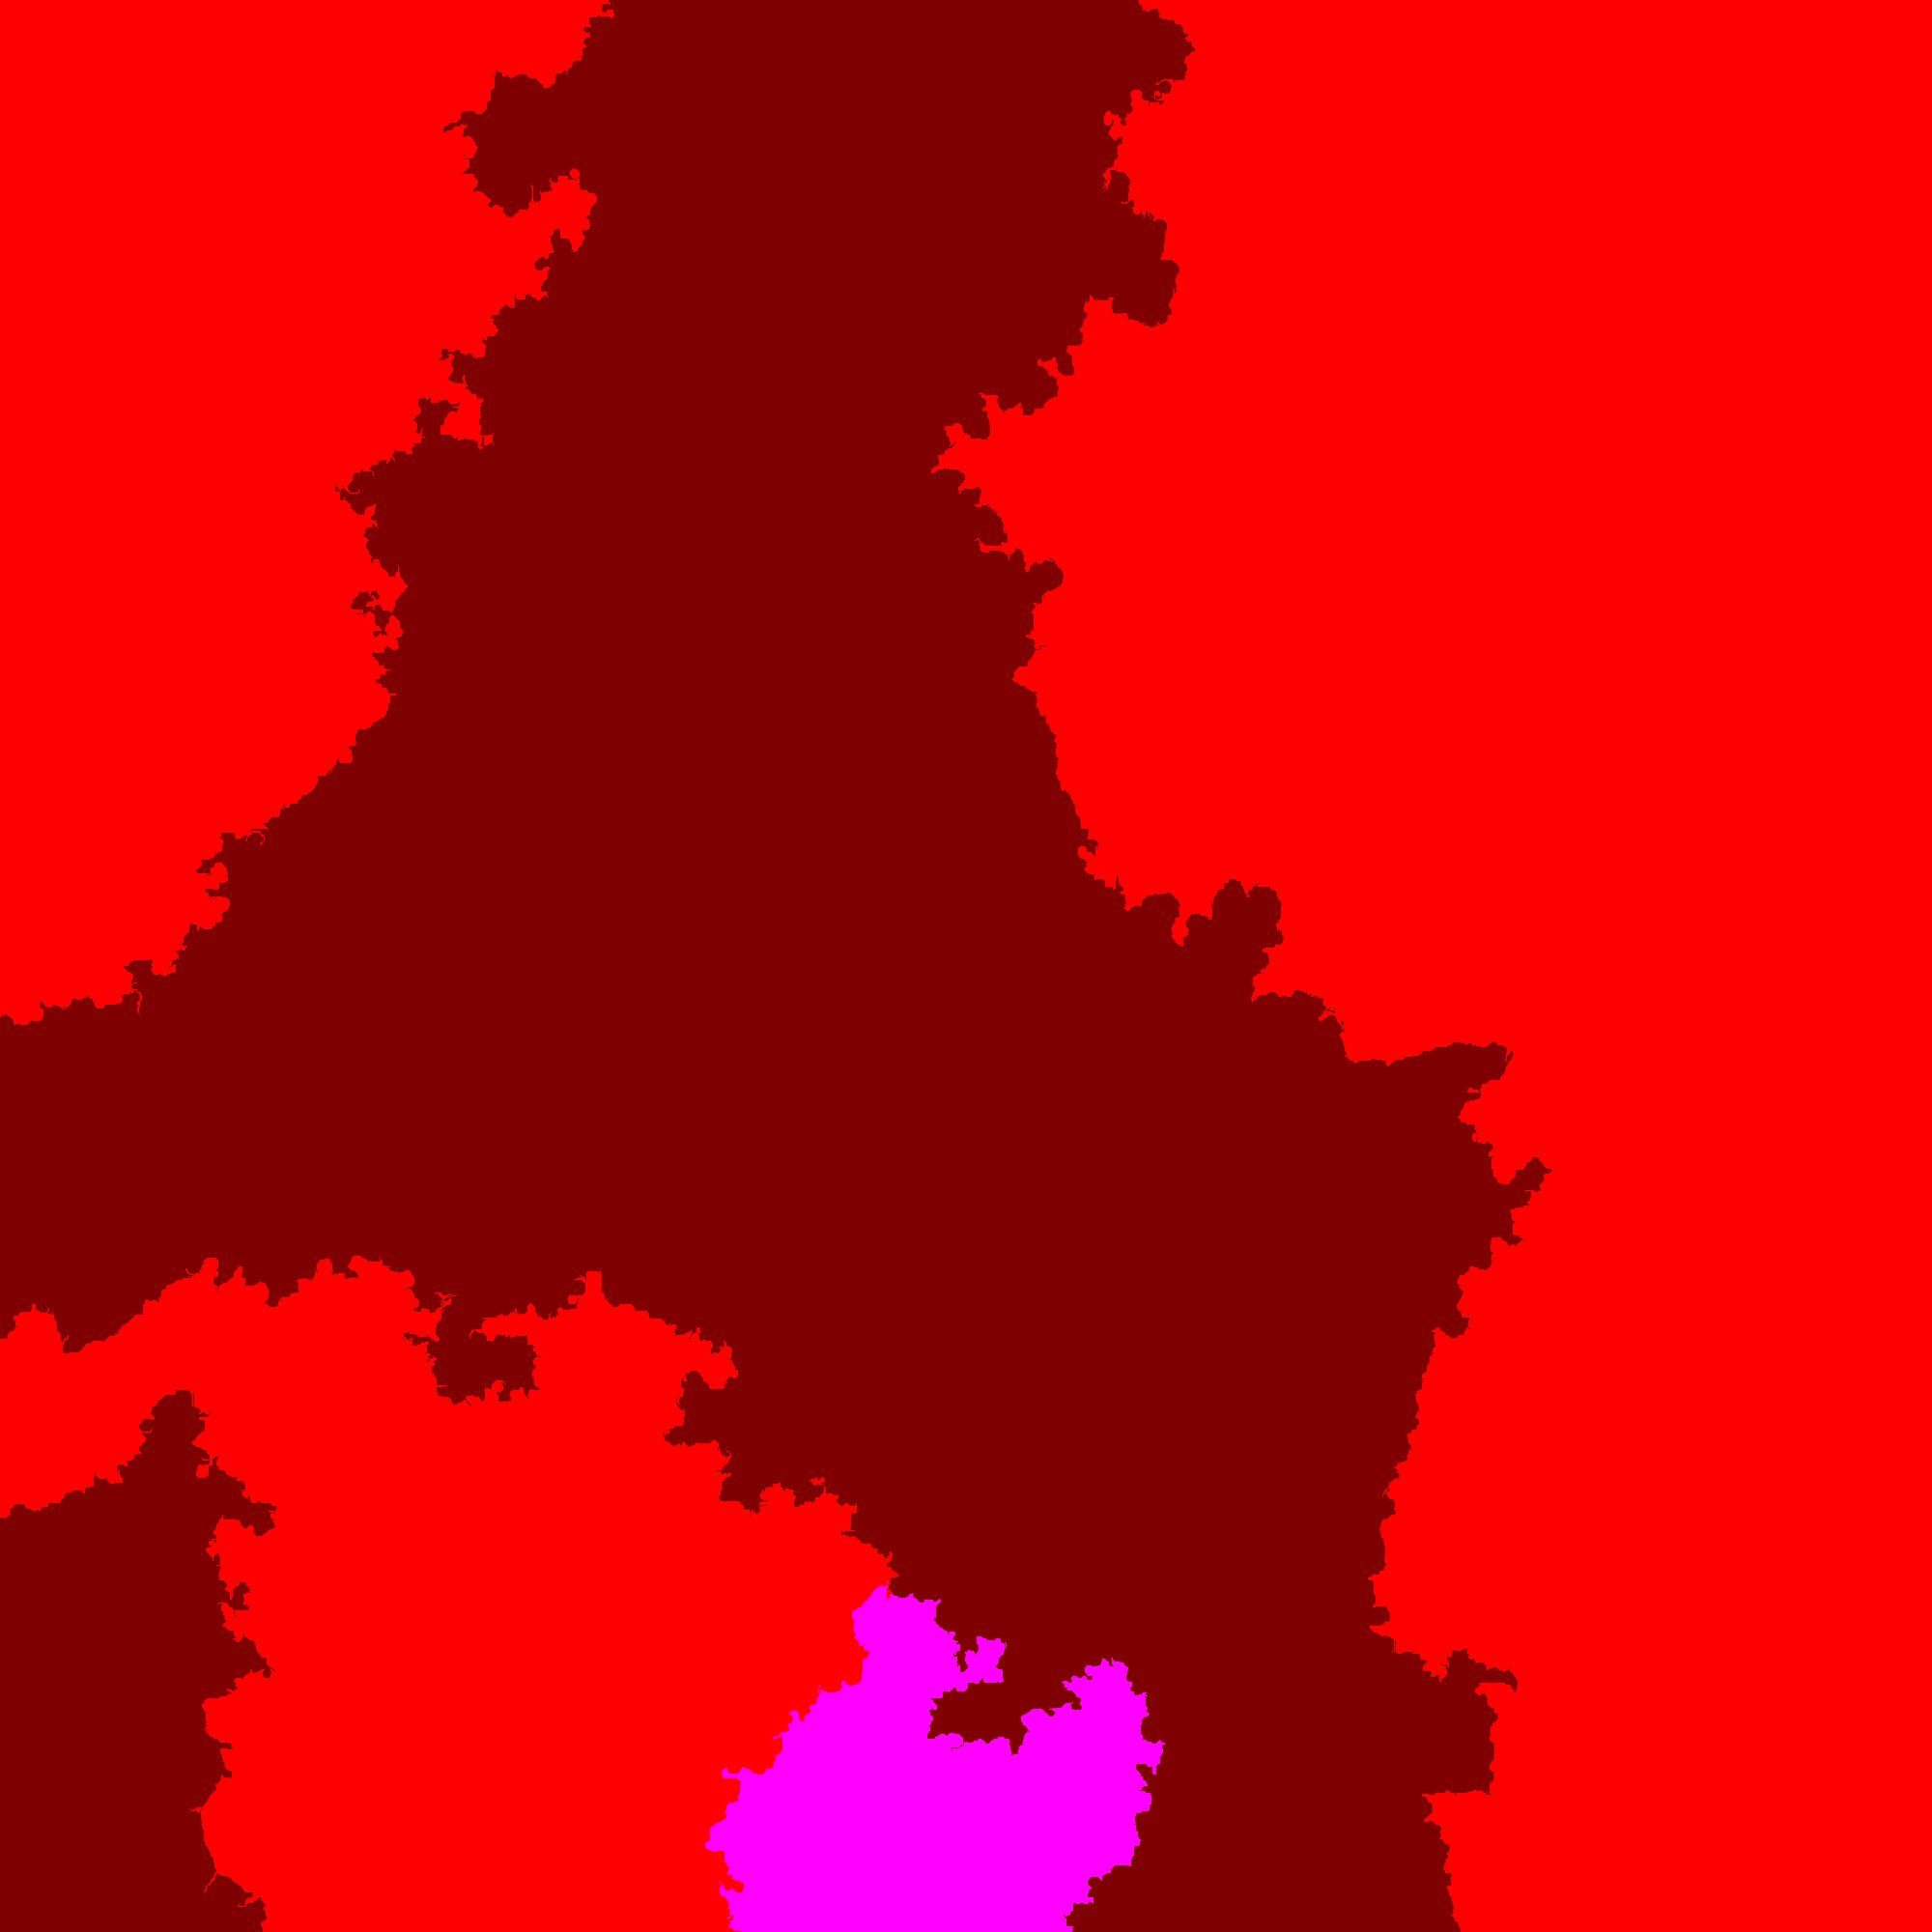
\includegraphics[width=0.3\textwidth]{Figures/C3/S2/seg_PFF_z_colored}
\label{subfig:seg_z_semc}
}
\endgroup
\caption{Results of the majority vote on the segmentation of the VHR optical images.}
\label{fig:seg_z_sem}
\end{center}
\end{figure}

The same results are observed, a majority vote applied to a segmentation equivalent to stands (in term of size) does not allow to retrieve a relevant mapping of forested areas. \\

From this section, two main conclusions can be drawn: firstly, the direct segmentation of the data does not allow to retrieve relevant forest stands in terms of species. Even with an addition of semantic information from a classification, the results are not sufficient for a mapping of the forest. Secondly, some metrics are not relevant in order to evaluate the results. Indeed, the overall accuracy or the $\kappa$ are not sufficient, other metrics are needed for the correct evaluation of the results.

\section{Results of the method}
The proposed method is composed of different steps (defined above). Each step will be evaluated at 2 levels; the direct output will be first considered and the impact on the final segmentation will also be investigated. In order to simplify the reading of captions, when no specific information is provided the method is employed using the following parameters:
\begin{itemize}
\item Feature selection:
\begin{itemize}
\item Selection of training samples,
\item Selection of 20 features,
\item Object-based features (lidar and spectral) obtained from the PFF over-segmentation,
\item Pixel-based features (lidar and spectral) for the regularization.
\end{itemize}
\item Classification performed with:
\begin{itemize}
\item Selection of training samples,
\item Object-based features (lidar and spectral) obtained from the feature selection.
\end{itemize}
\item Regularization using global method with:
\begin{itemize}
\item $\gamma=10$,
\item Linear data formulation,
\item \textit{Exponential-features model} with pixel-based features obtained from the feature selection.
\end{itemize}
\end{itemize}
\subsection{Over-segmentation}
\label{sec:C3_S3_ss1}
The results of the over-segmentation of proposed segmentation algorithms are presented in Figure~\ref{fig:C3_S3_ss1_seg}.

\begin{figure}[htbp]
\begin{center}
\begingroup
\captionsetup[subfigure]{width=0.325\textwidth}
\subfloat[RGB VHR optical image (250$\:$m$\times$250$\:$m).]{
\includegraphics[width=0.465\textwidth]{Figures/C3/S3/ss1/RGB}
\label{subfig:C3_S3_ss1_sega}
}
\hspace*{0.025\textwidth}
\subfloat[nDSM.]{
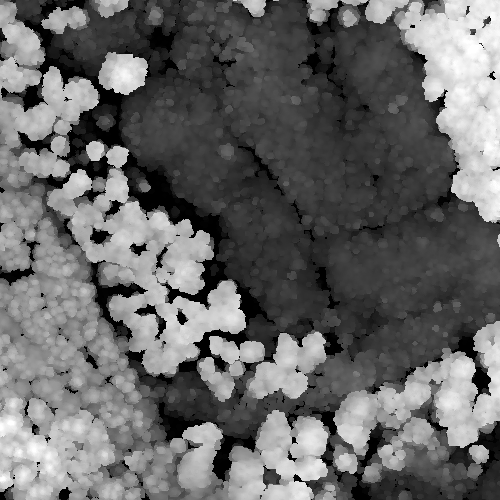
\includegraphics[width=0.465\textwidth]{Figures/C3/S3/ss1/nDSM}
\label{subfig:C3_S3_ss1_segb}
}
\endgroup
\\
\begingroup
\captionsetup[subfigure]{width=0.3\textwidth}
\subfloat[Tree extraction.]{
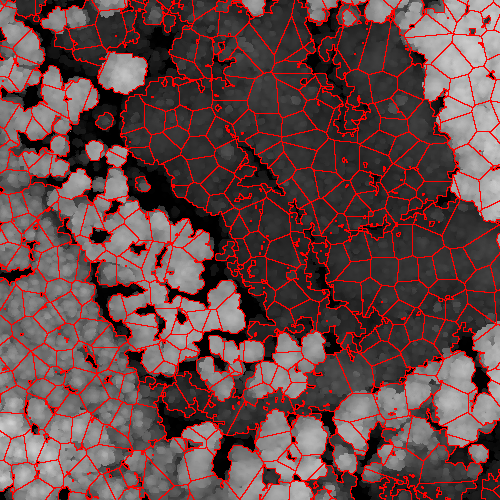
\includegraphics[width=0.3\textwidth]{Figures/C3/S3/ss1/nDSM_tree}
\label{subfig:C3_S3_ss1_segc}
}
\hspace*{0.025\textwidth}
\subfloat[Watershed.]{
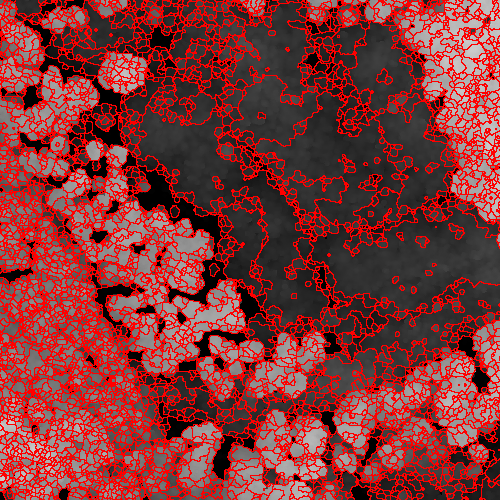
\includegraphics[width=0.3\textwidth]{Figures/C3/S3/ss1/nDSM_watershed}
\label{subfig:C3_S3_ss1_segd}
}
\hspace*{0.025\textwidth}
\subfloat[Hierarchical segmentation.]{
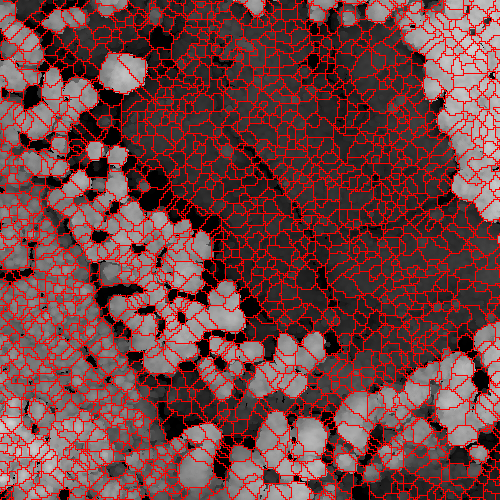
\includegraphics[width=0.3\textwidth]{Figures/C3/S3/ss1/nDSM_hierarchical}
\label{subfig:C3_S3_ss1_sege}
}
\\
\subfloat[PFF.]{
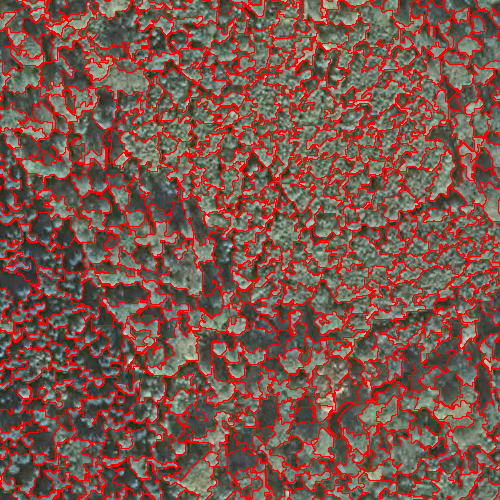
\includegraphics[width=0.3\textwidth]{Figures/C3/S3/ss1/PFF}
\label{subfig:C3_S3_ss1_segf}
}
\hspace*{0.025\textwidth}
\subfloat[Quickshift.]{
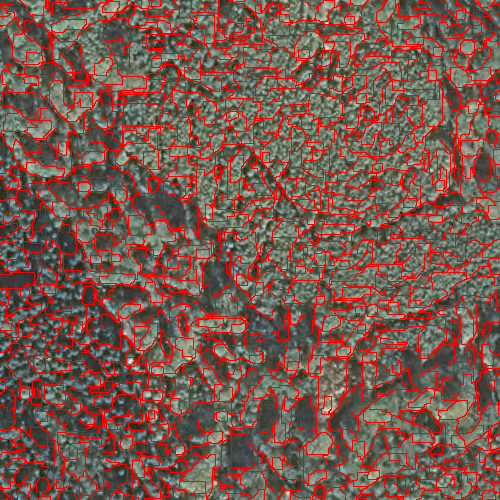
\includegraphics[width=0.3\textwidth]{Figures/C3/S3/ss1/quickshift}
\label{subfig:C3_S3_ss1_segg}
}
\hspace*{0.025\textwidth}
\subfloat[SLIC.]{
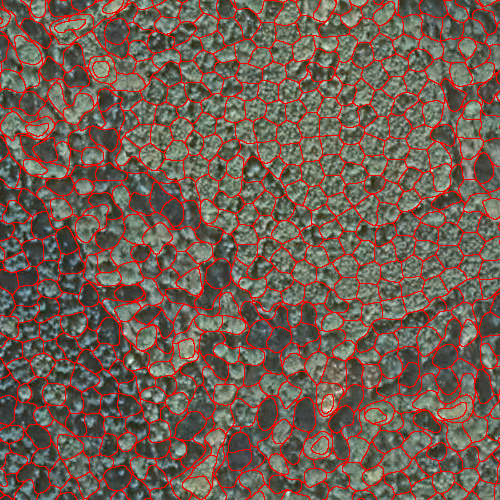
\includegraphics[width=0.3\textwidth]{Figures/C3/S3/ss1/SLIC}
\label{subfig:C3_S3_ss1_segh}
}

\endgroup
\caption{Over segmentation results, red corresponds to the borders found by the segmentation algorithm.}
\label{fig:C3_S3_ss1_seg}
\end{center}
\end{figure}

In all the proposed methods, the resulting segments are relevant since the all represent small homogeneous objects. The object are mostly not of the same size and shape, except for the SLIC superpixels (the aims of the methods is to obtain such uniform segments). The PFF algorithm produces objects with rough borders that are following precisely the borders observed on the images. From a visual point of view, it appears that there is no segmentation method that performs better than the others. Furthermore, it is impossible to evaluate the segmentation since no ground truth is available. Thus, the different segmentation methods are compared through the results they produce after the object-based classification (which indicates how the objects are relevant for classification) and after the regularization (how the objects impacts the final results). These results are presented in Figure~\ref{fig:C3_S3_ss1_results}\\

\begin{figure}[htbp]
\begin{center}
\begingroup
\captionsetup[subfigure]{width=0.21\textwidth}
\subfloat[IRC VHR \hbox{optical image}.]{
\includegraphics[width=0.3\textwidth]{Figures/C3/S3/ss1/classif_regul/IRC}
\label{subfig:C3_S3_ss1_resultsa}
}
\hspace*{0.025\textwidth}
\subfloat[nDSM.]{
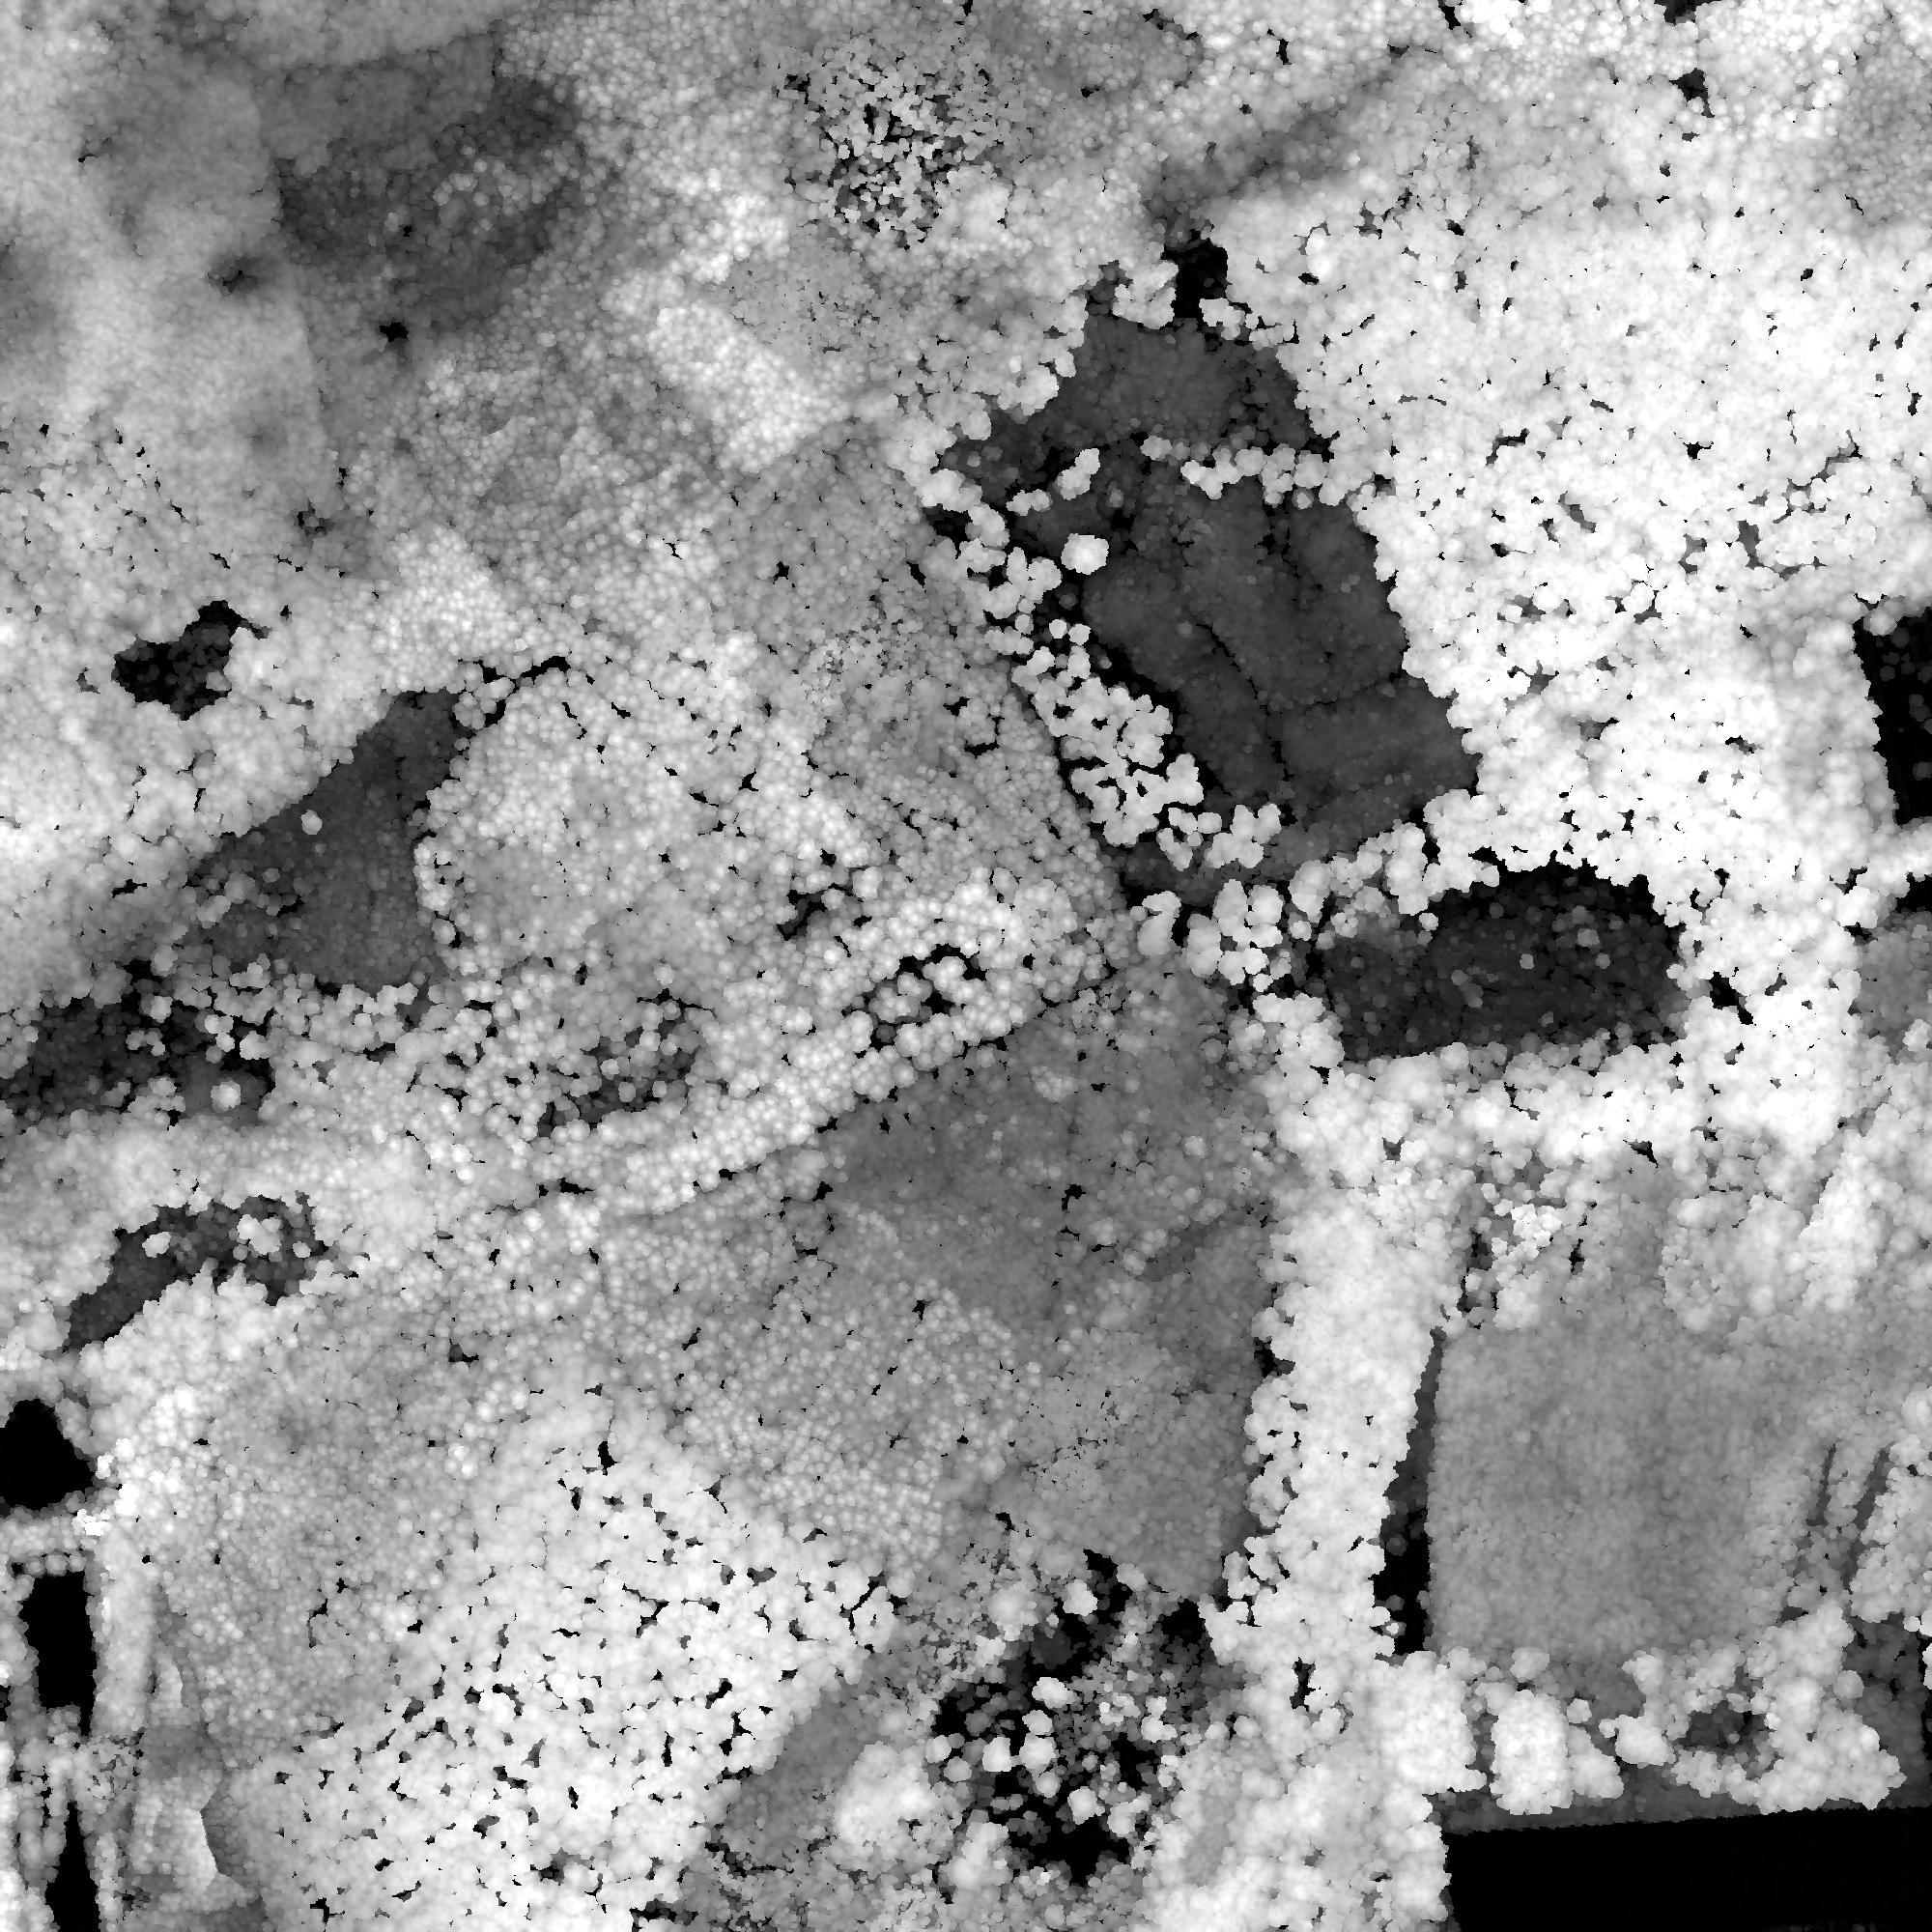
\includegraphics[width=0.3\textwidth]{Figures/C3/S3/ss1/classif_regul/nDSM}
\label{subfig:C3_S3_ss1_resultsb}
}
\hspace*{0.025\textwidth}
\subfloat[Forest LC.]{
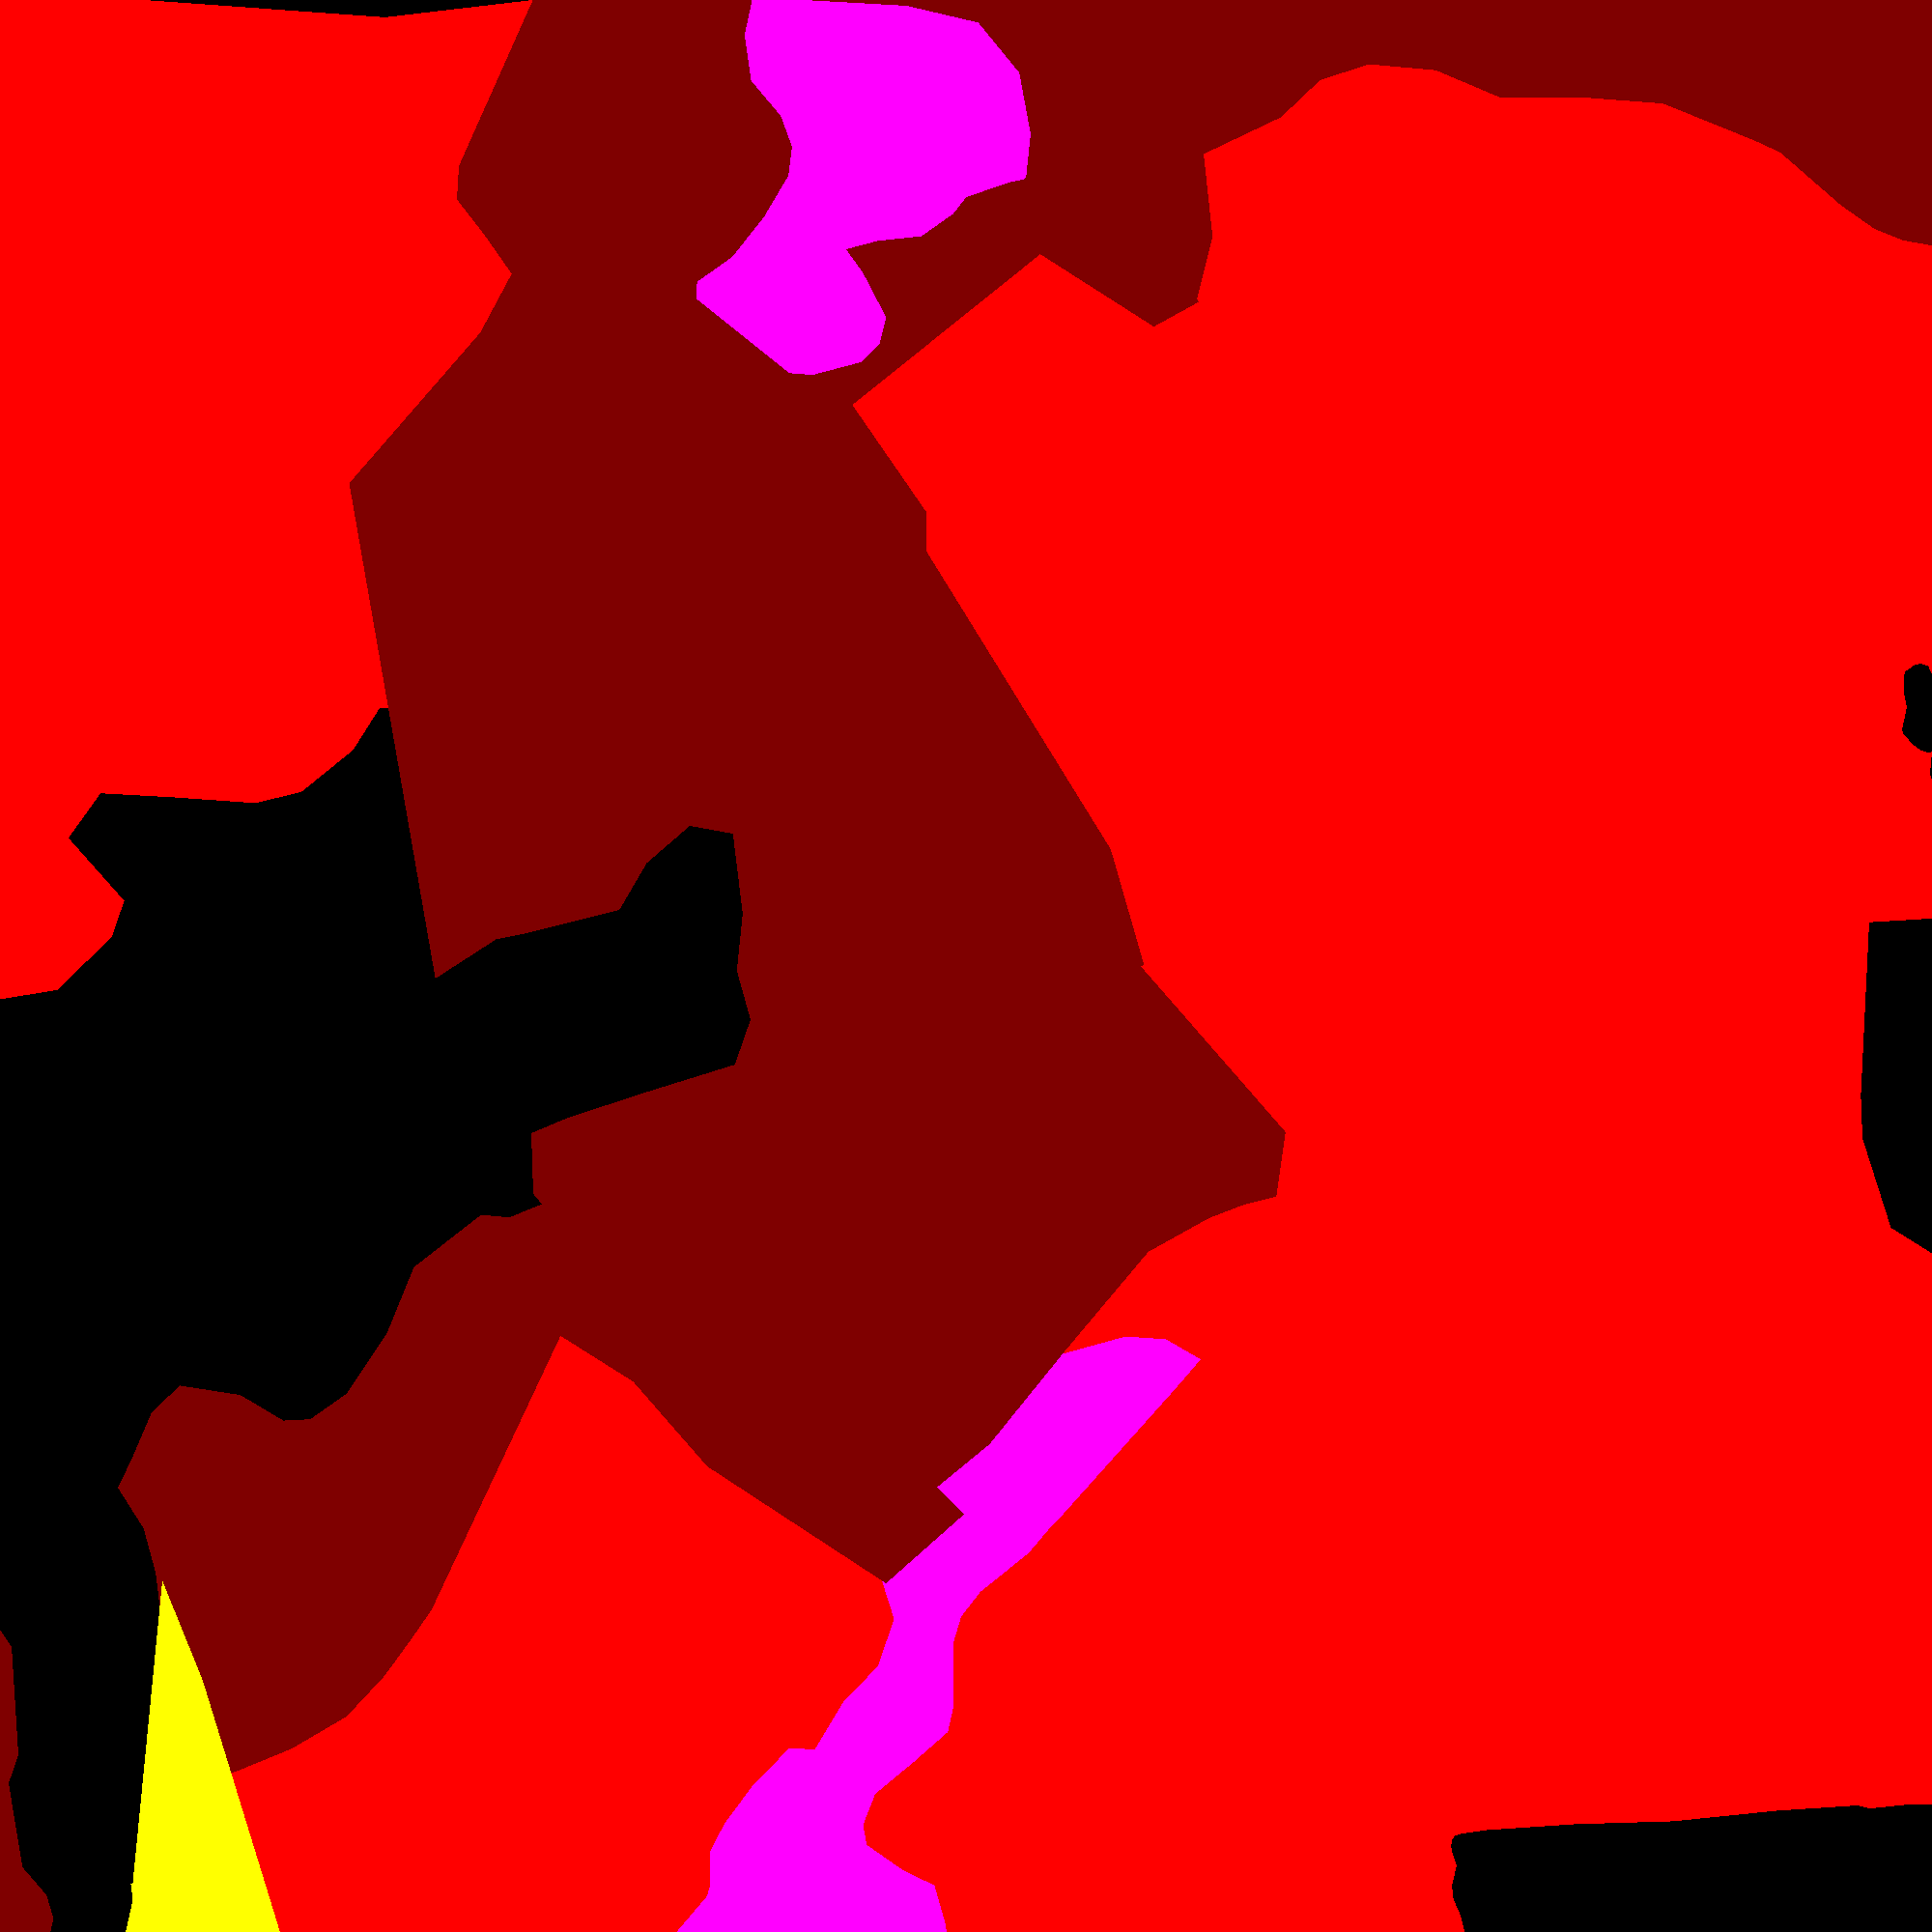
\includegraphics[width=0.3\textwidth]{Figures/C3/S3/ss1/classif_regul/BD}
\label{subfig:C3_S3_ss1_resultsc}
}
\\
\subfloat[Tree extraction.]{
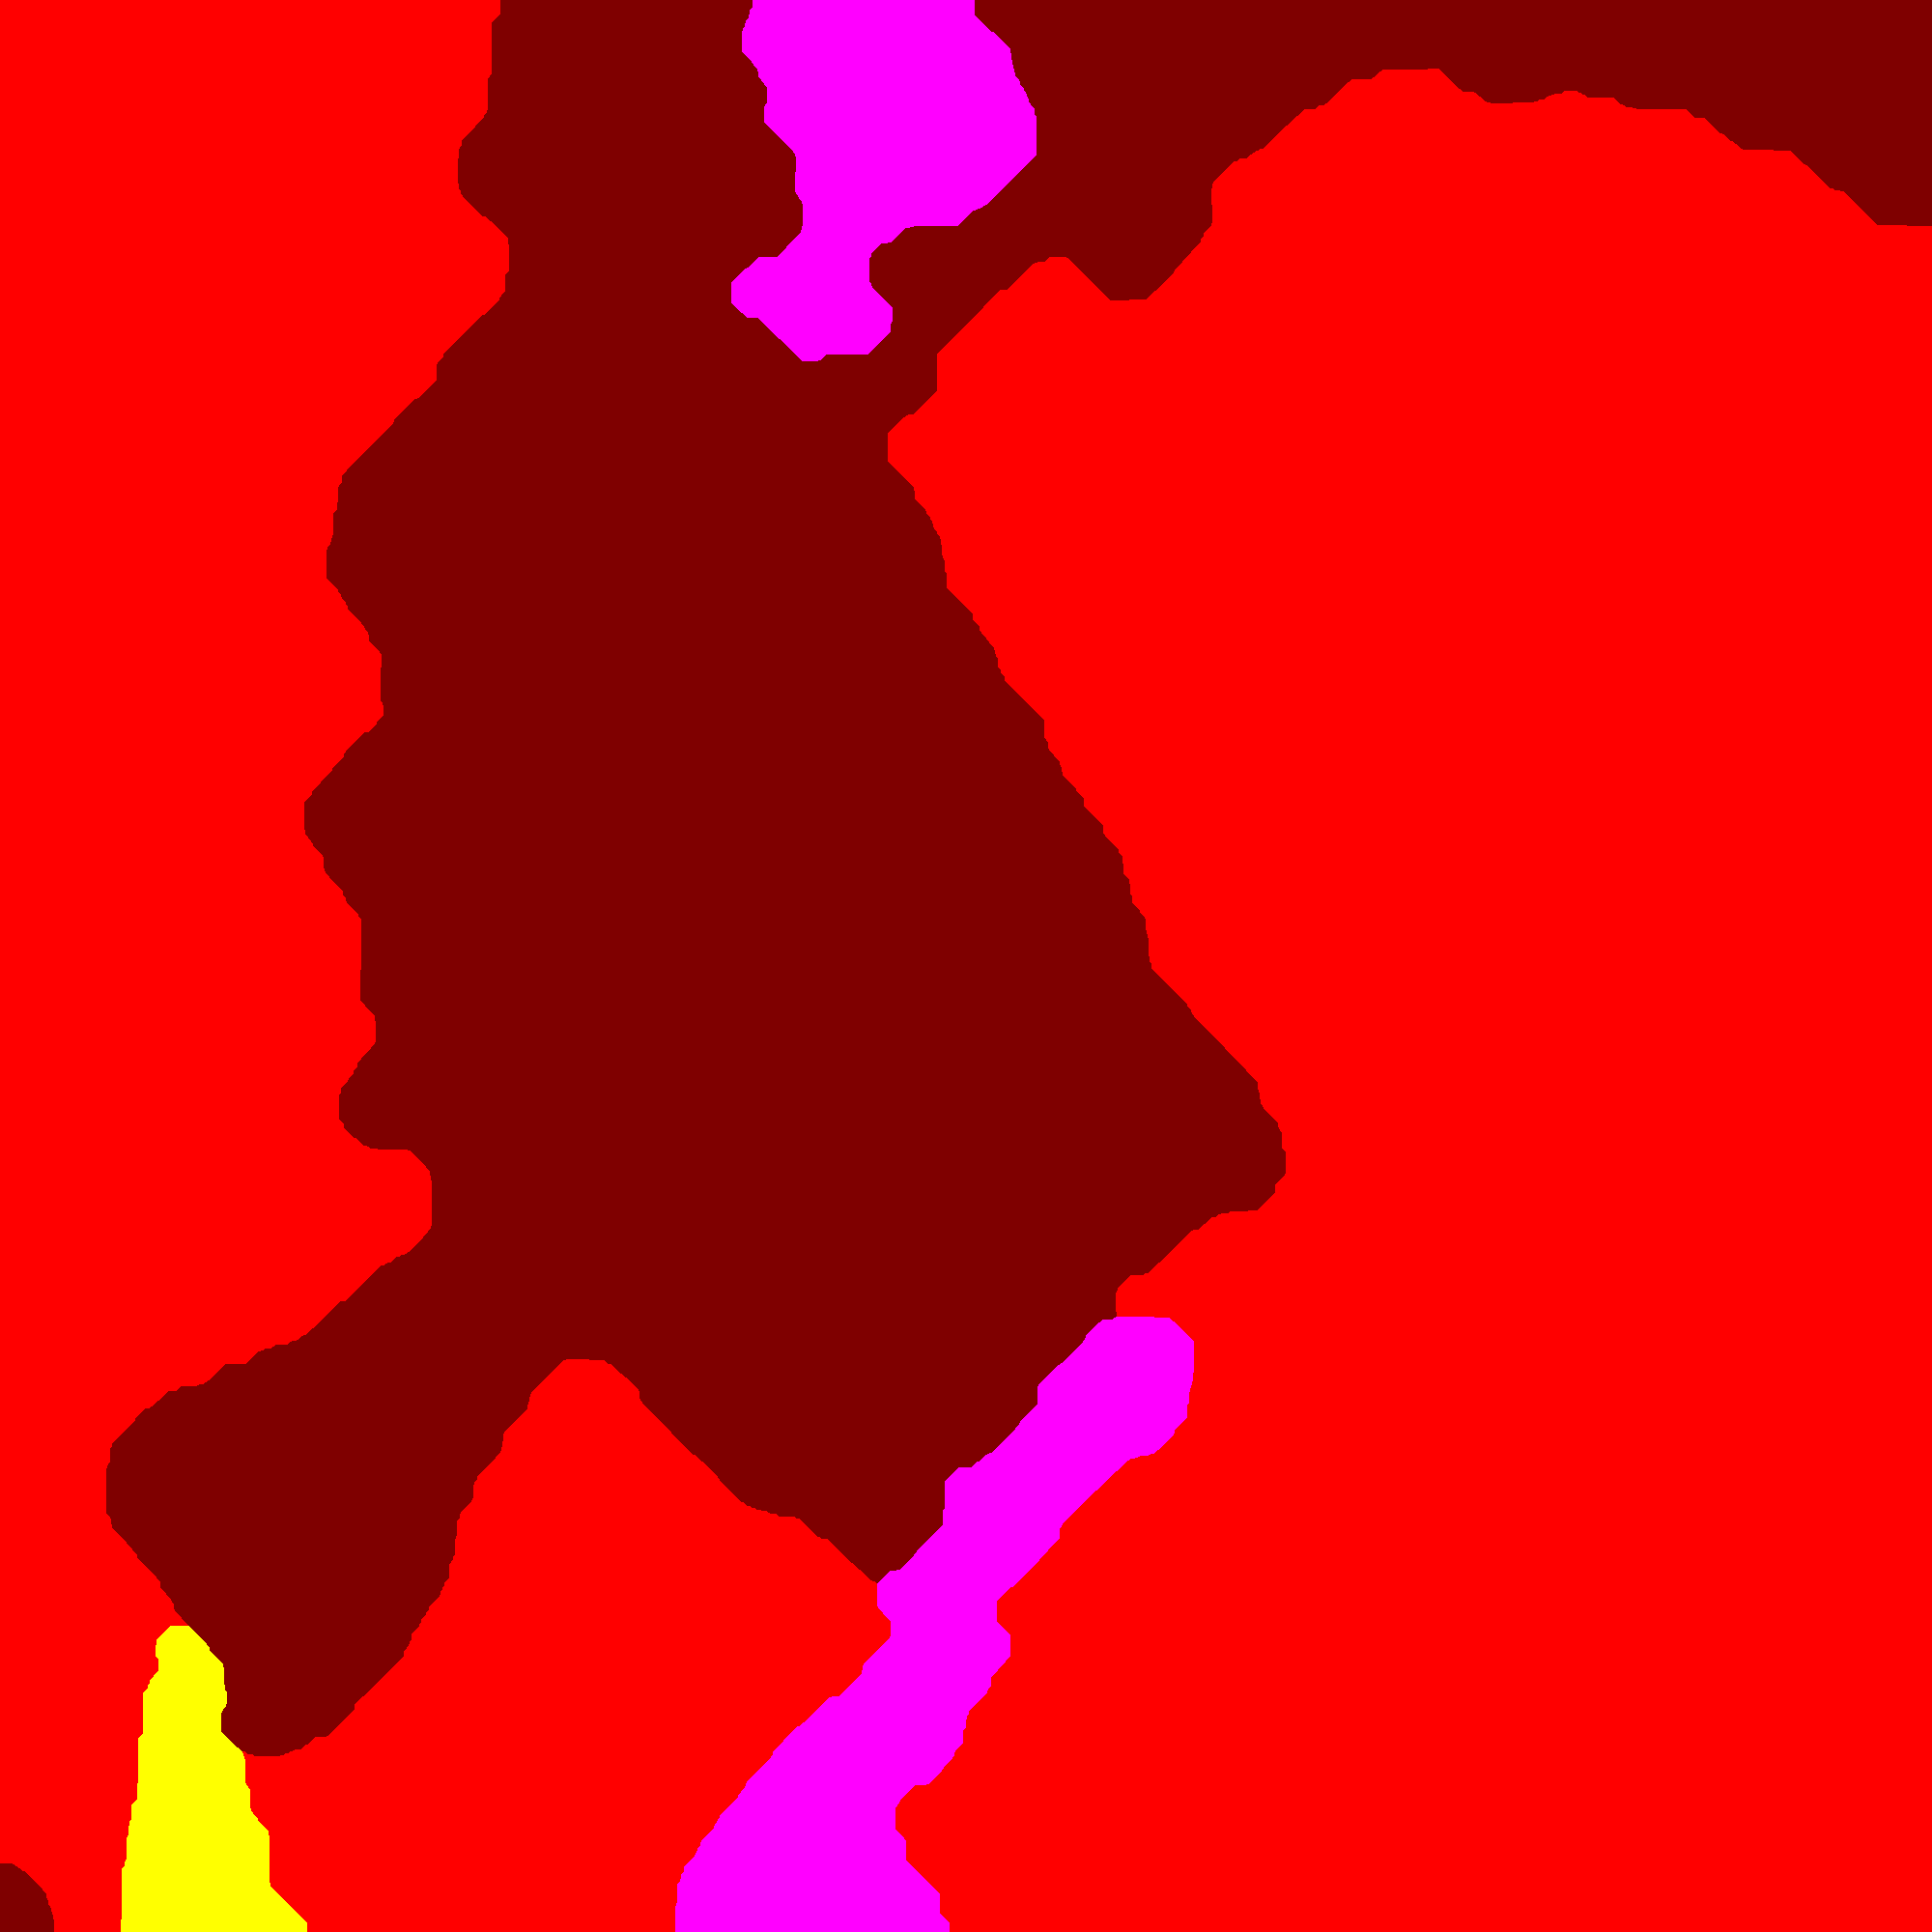
\includegraphics[width=0.3\textwidth]{Figures/C3/S3/ss1/classif_regul/trees/regul}
\label{subfig:C3_S3_ss1_resultsd}
}
\hspace*{0.025\textwidth}
\subfloat[Watershed.]{
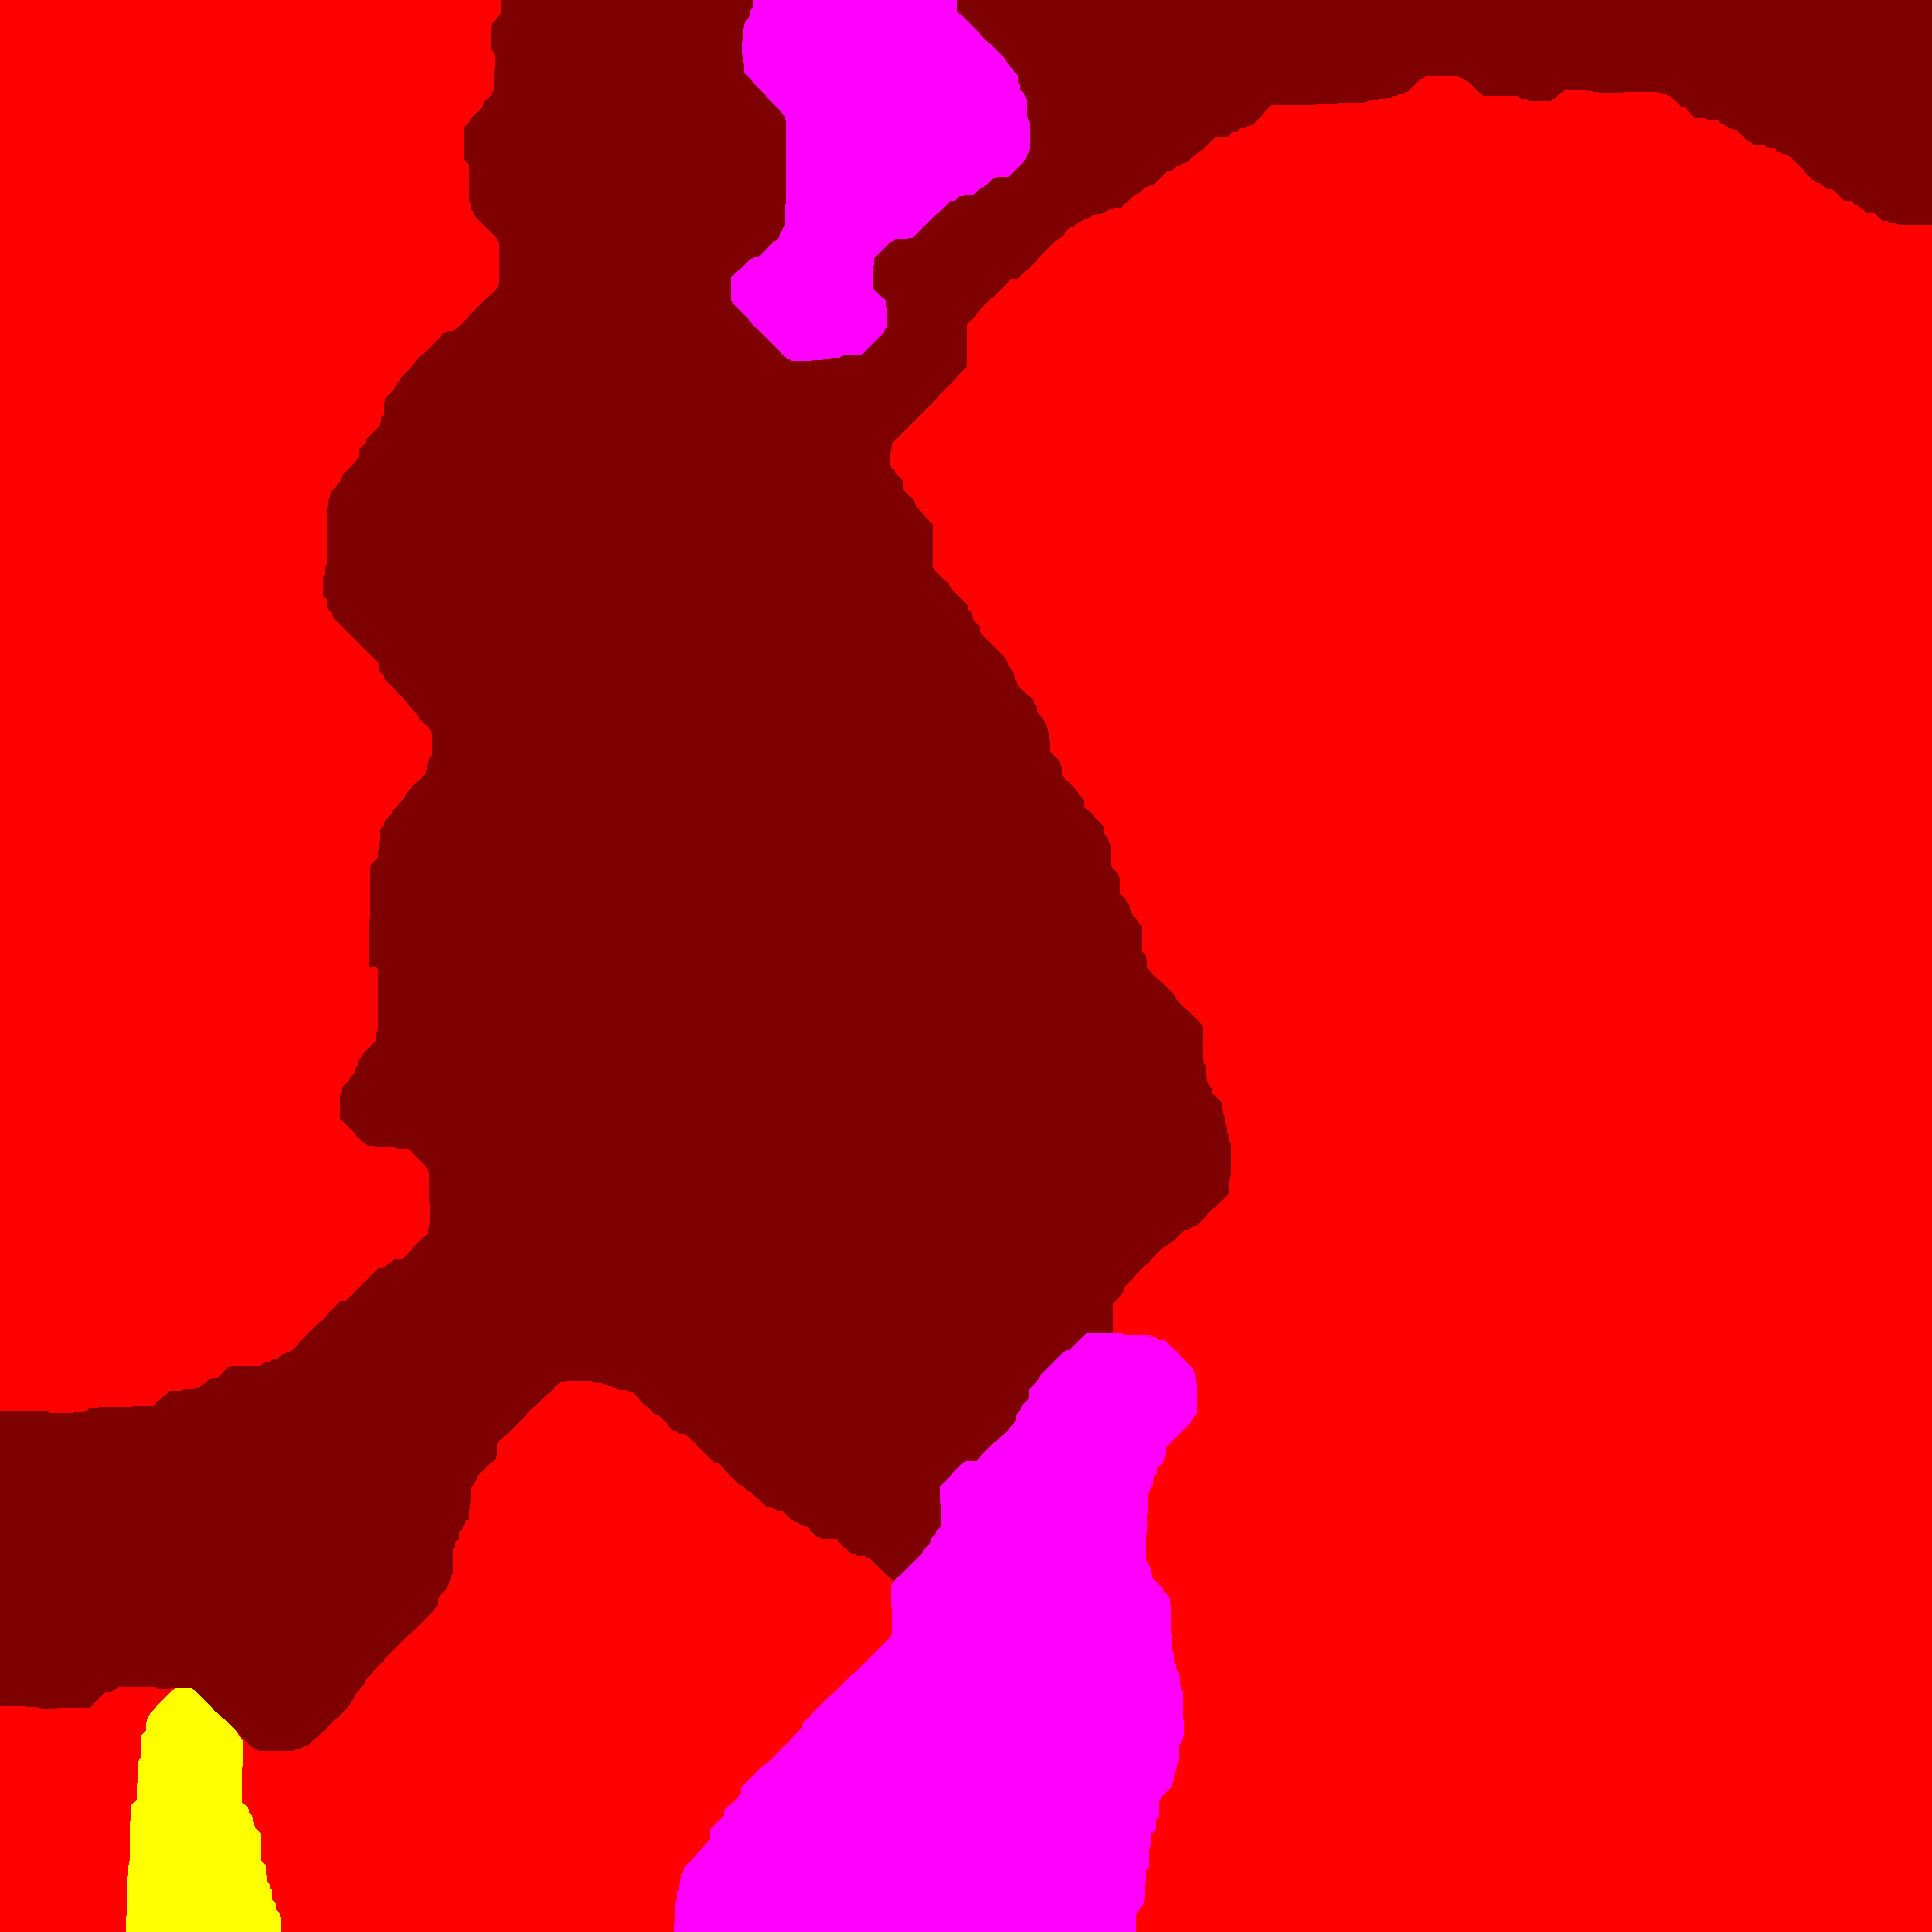
\includegraphics[width=0.3\textwidth]{Figures/C3/S3/ss1/classif_regul/watershed/regul}
\label{subfig:C3_S3_ss1_resultse}
}
\hspace*{0.025\textwidth}
\subfloat[Hierarchical \hbox{segmentation}.]{
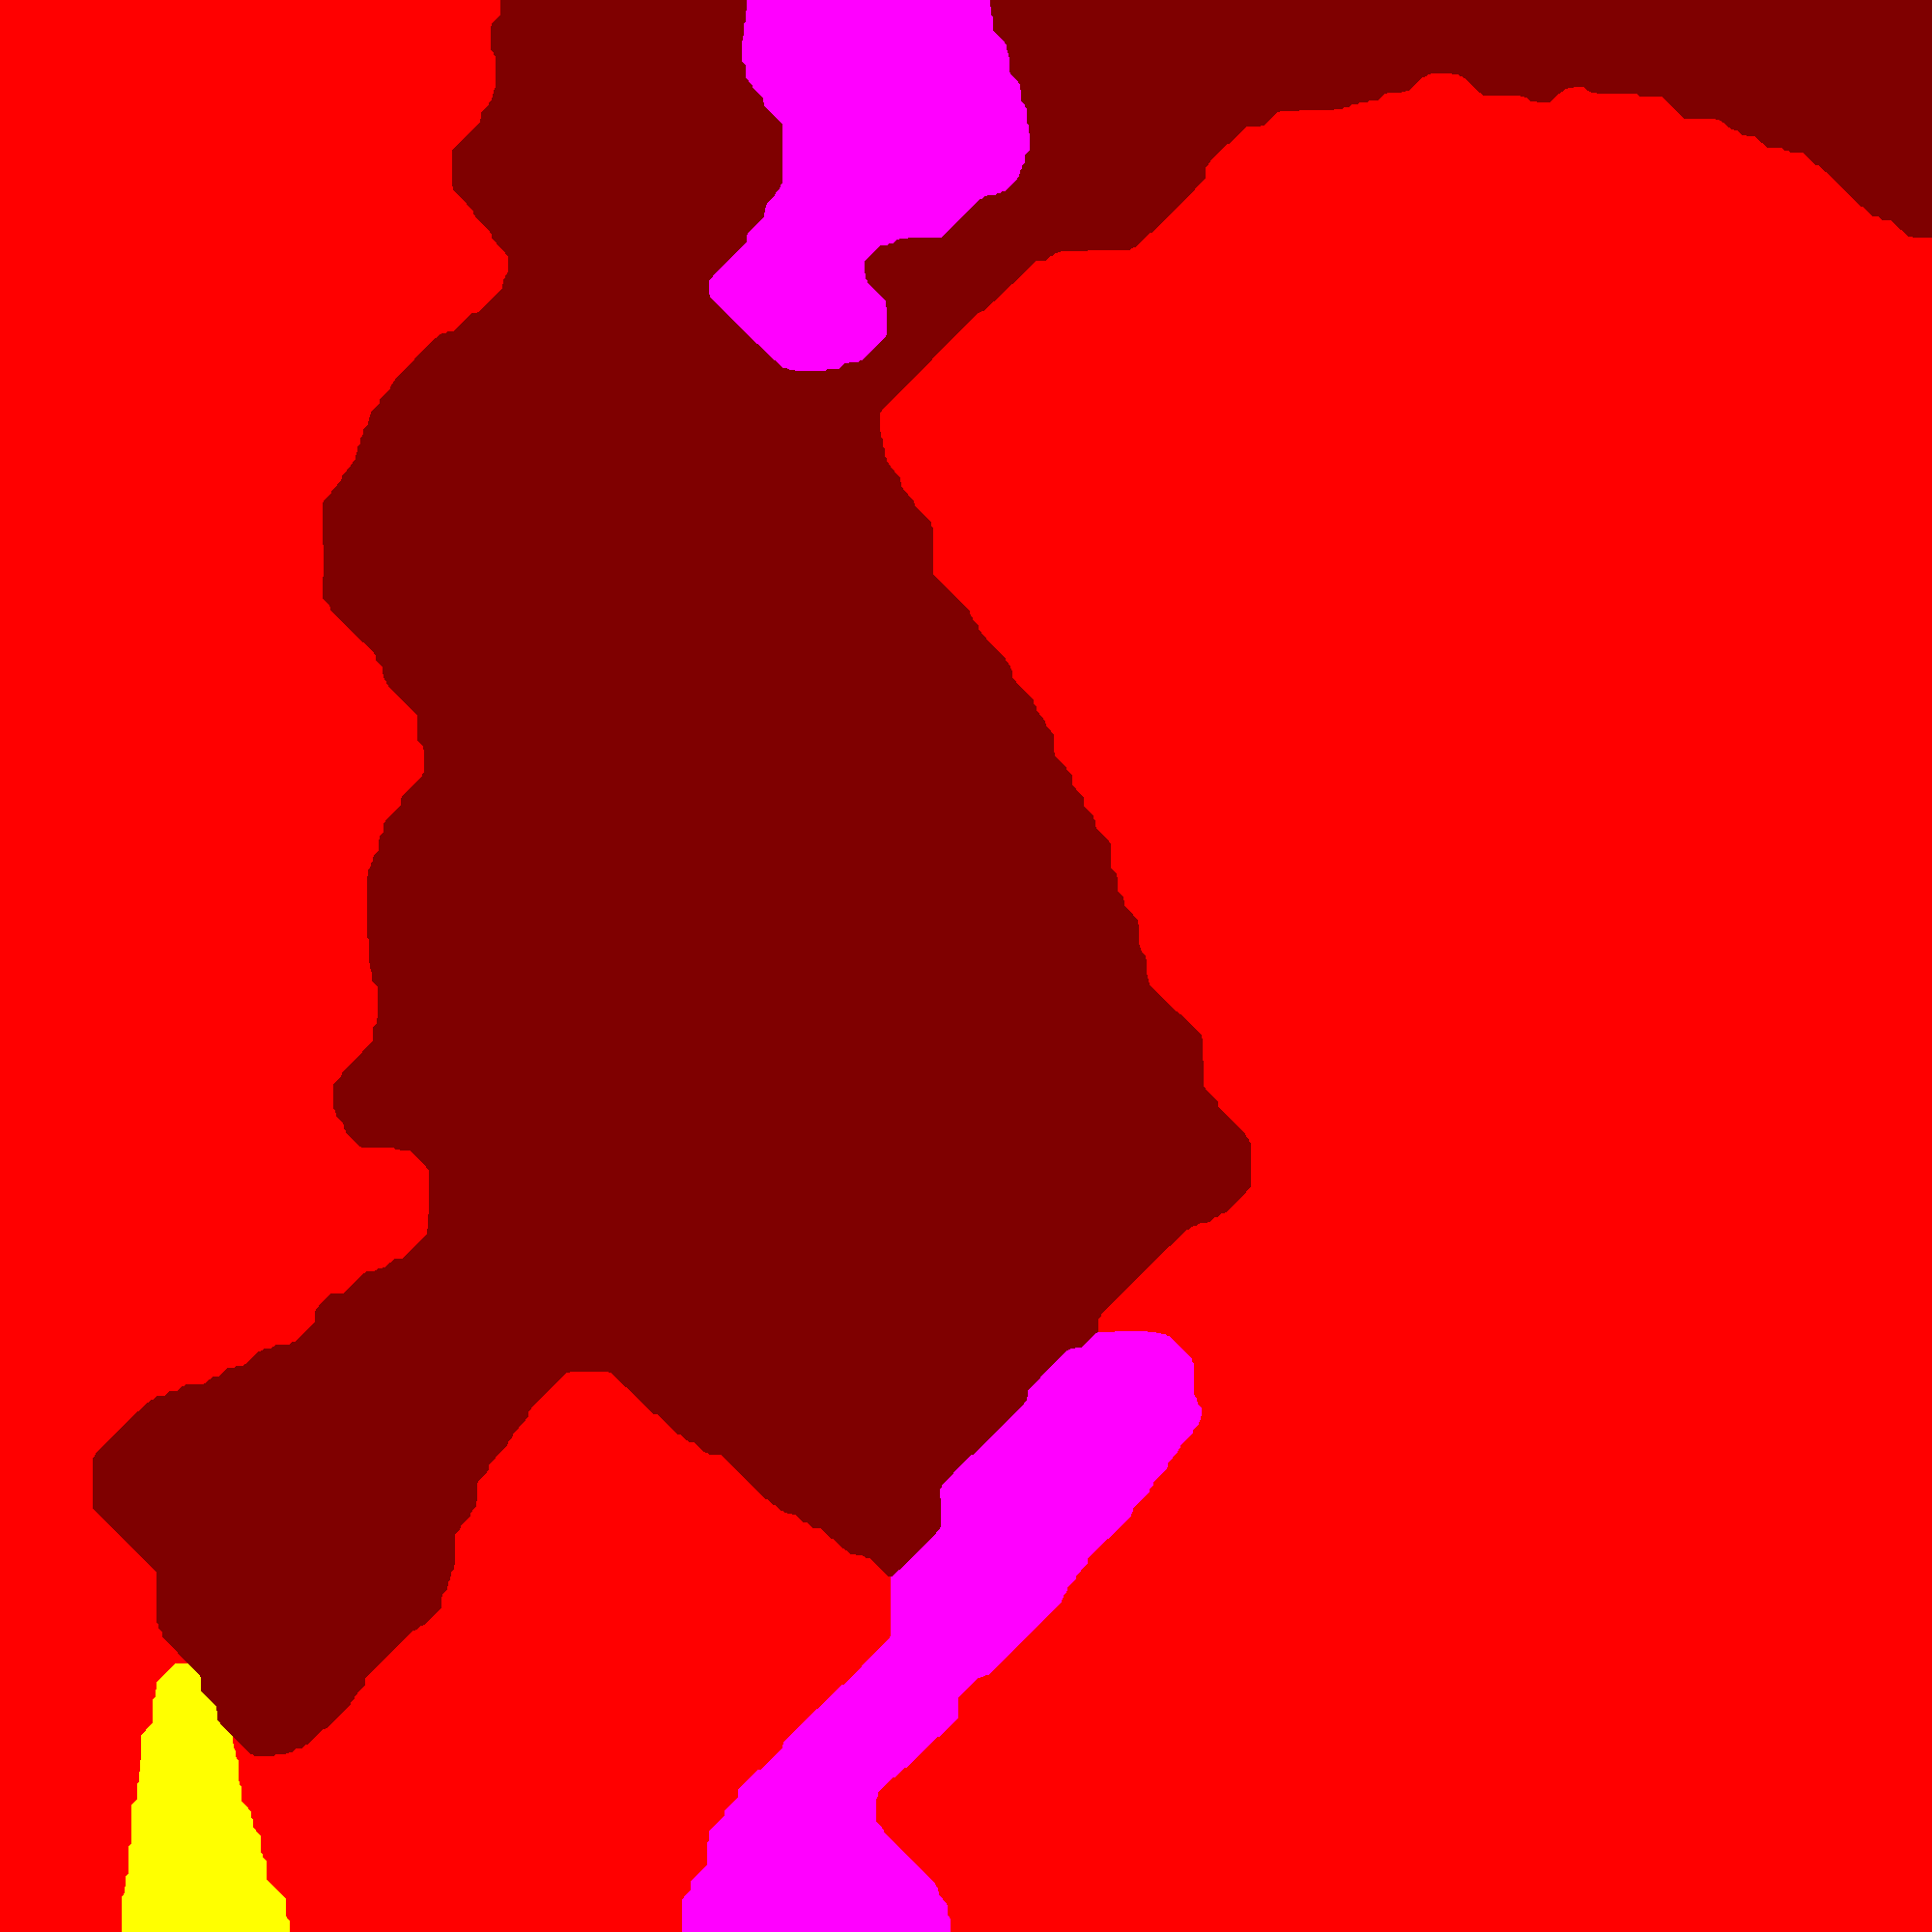
\includegraphics[width=0.3\textwidth]{Figures/C3/S3/ss1/classif_regul/hierarchical/regul}
\label{subfig:C3_S3_ss1_resultsf}
}
\\
\subfloat[PFF.]{
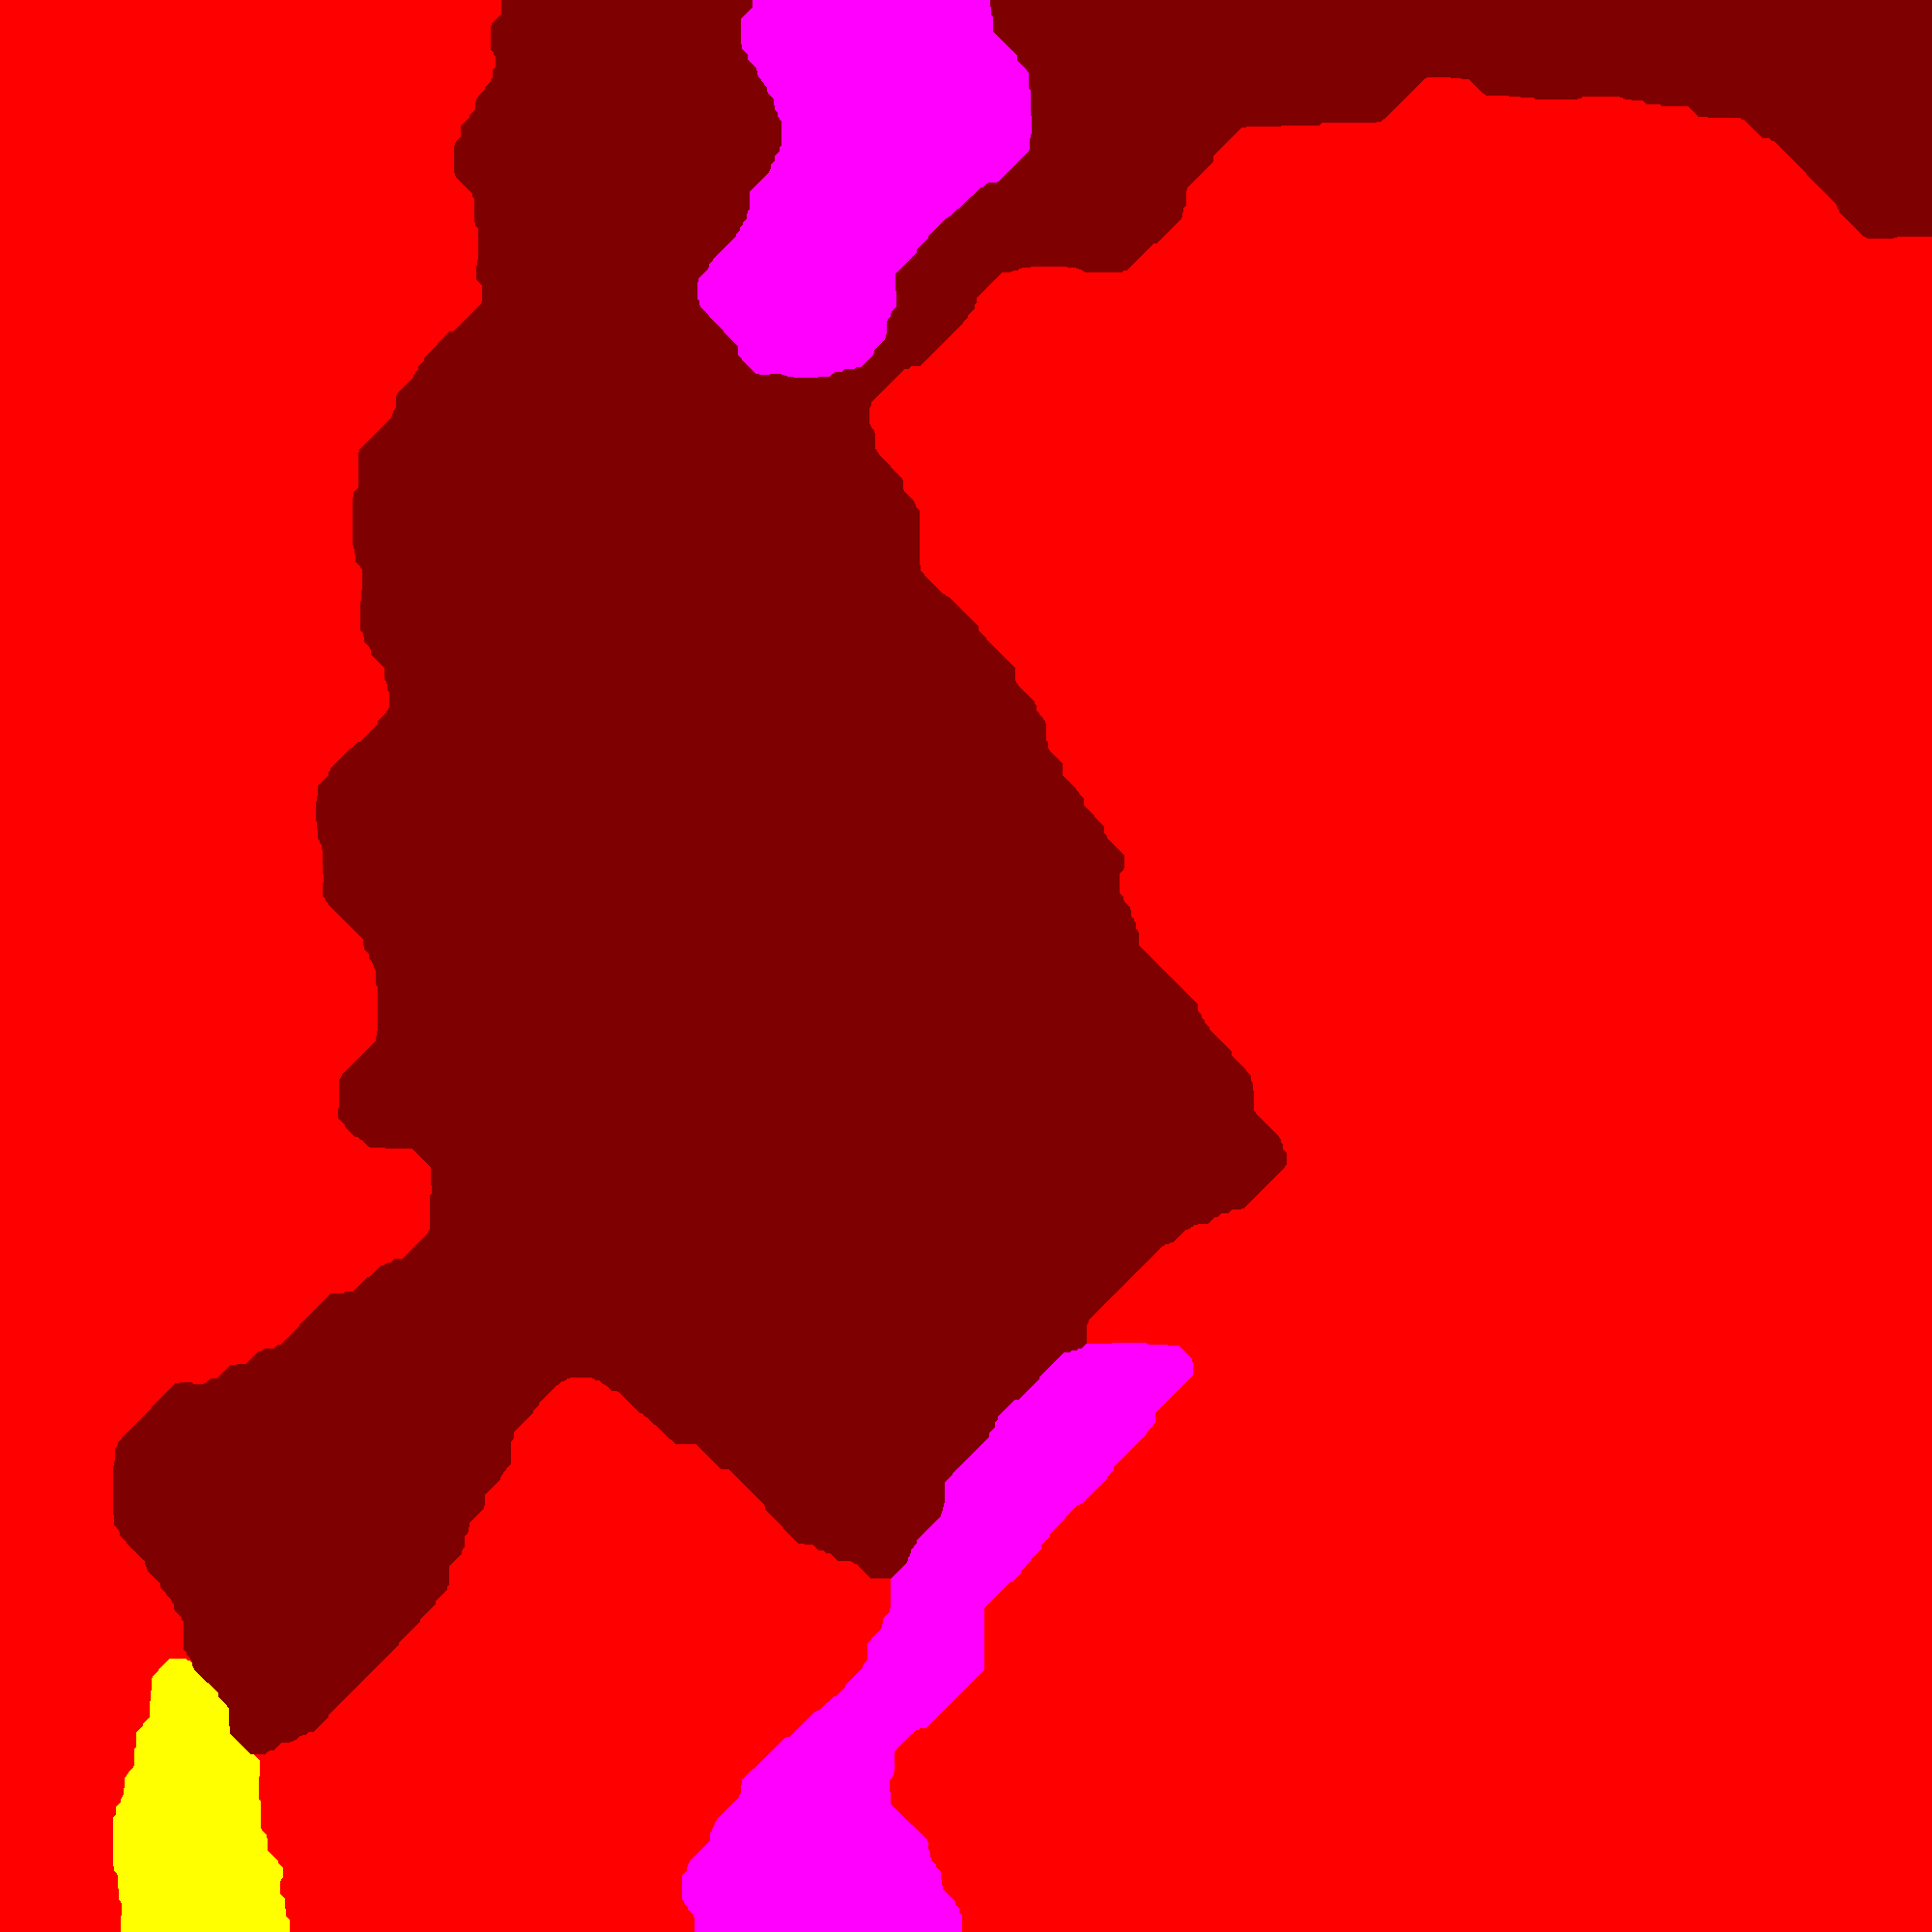
\includegraphics[width=0.3\textwidth]{Figures/C3/S3/ss1/classif_regul/PFF/regul}
\label{subfig:C3_S3_ss1_resultsg}
}
\hspace*{0.025\textwidth}
\subfloat[Quickshift.]{
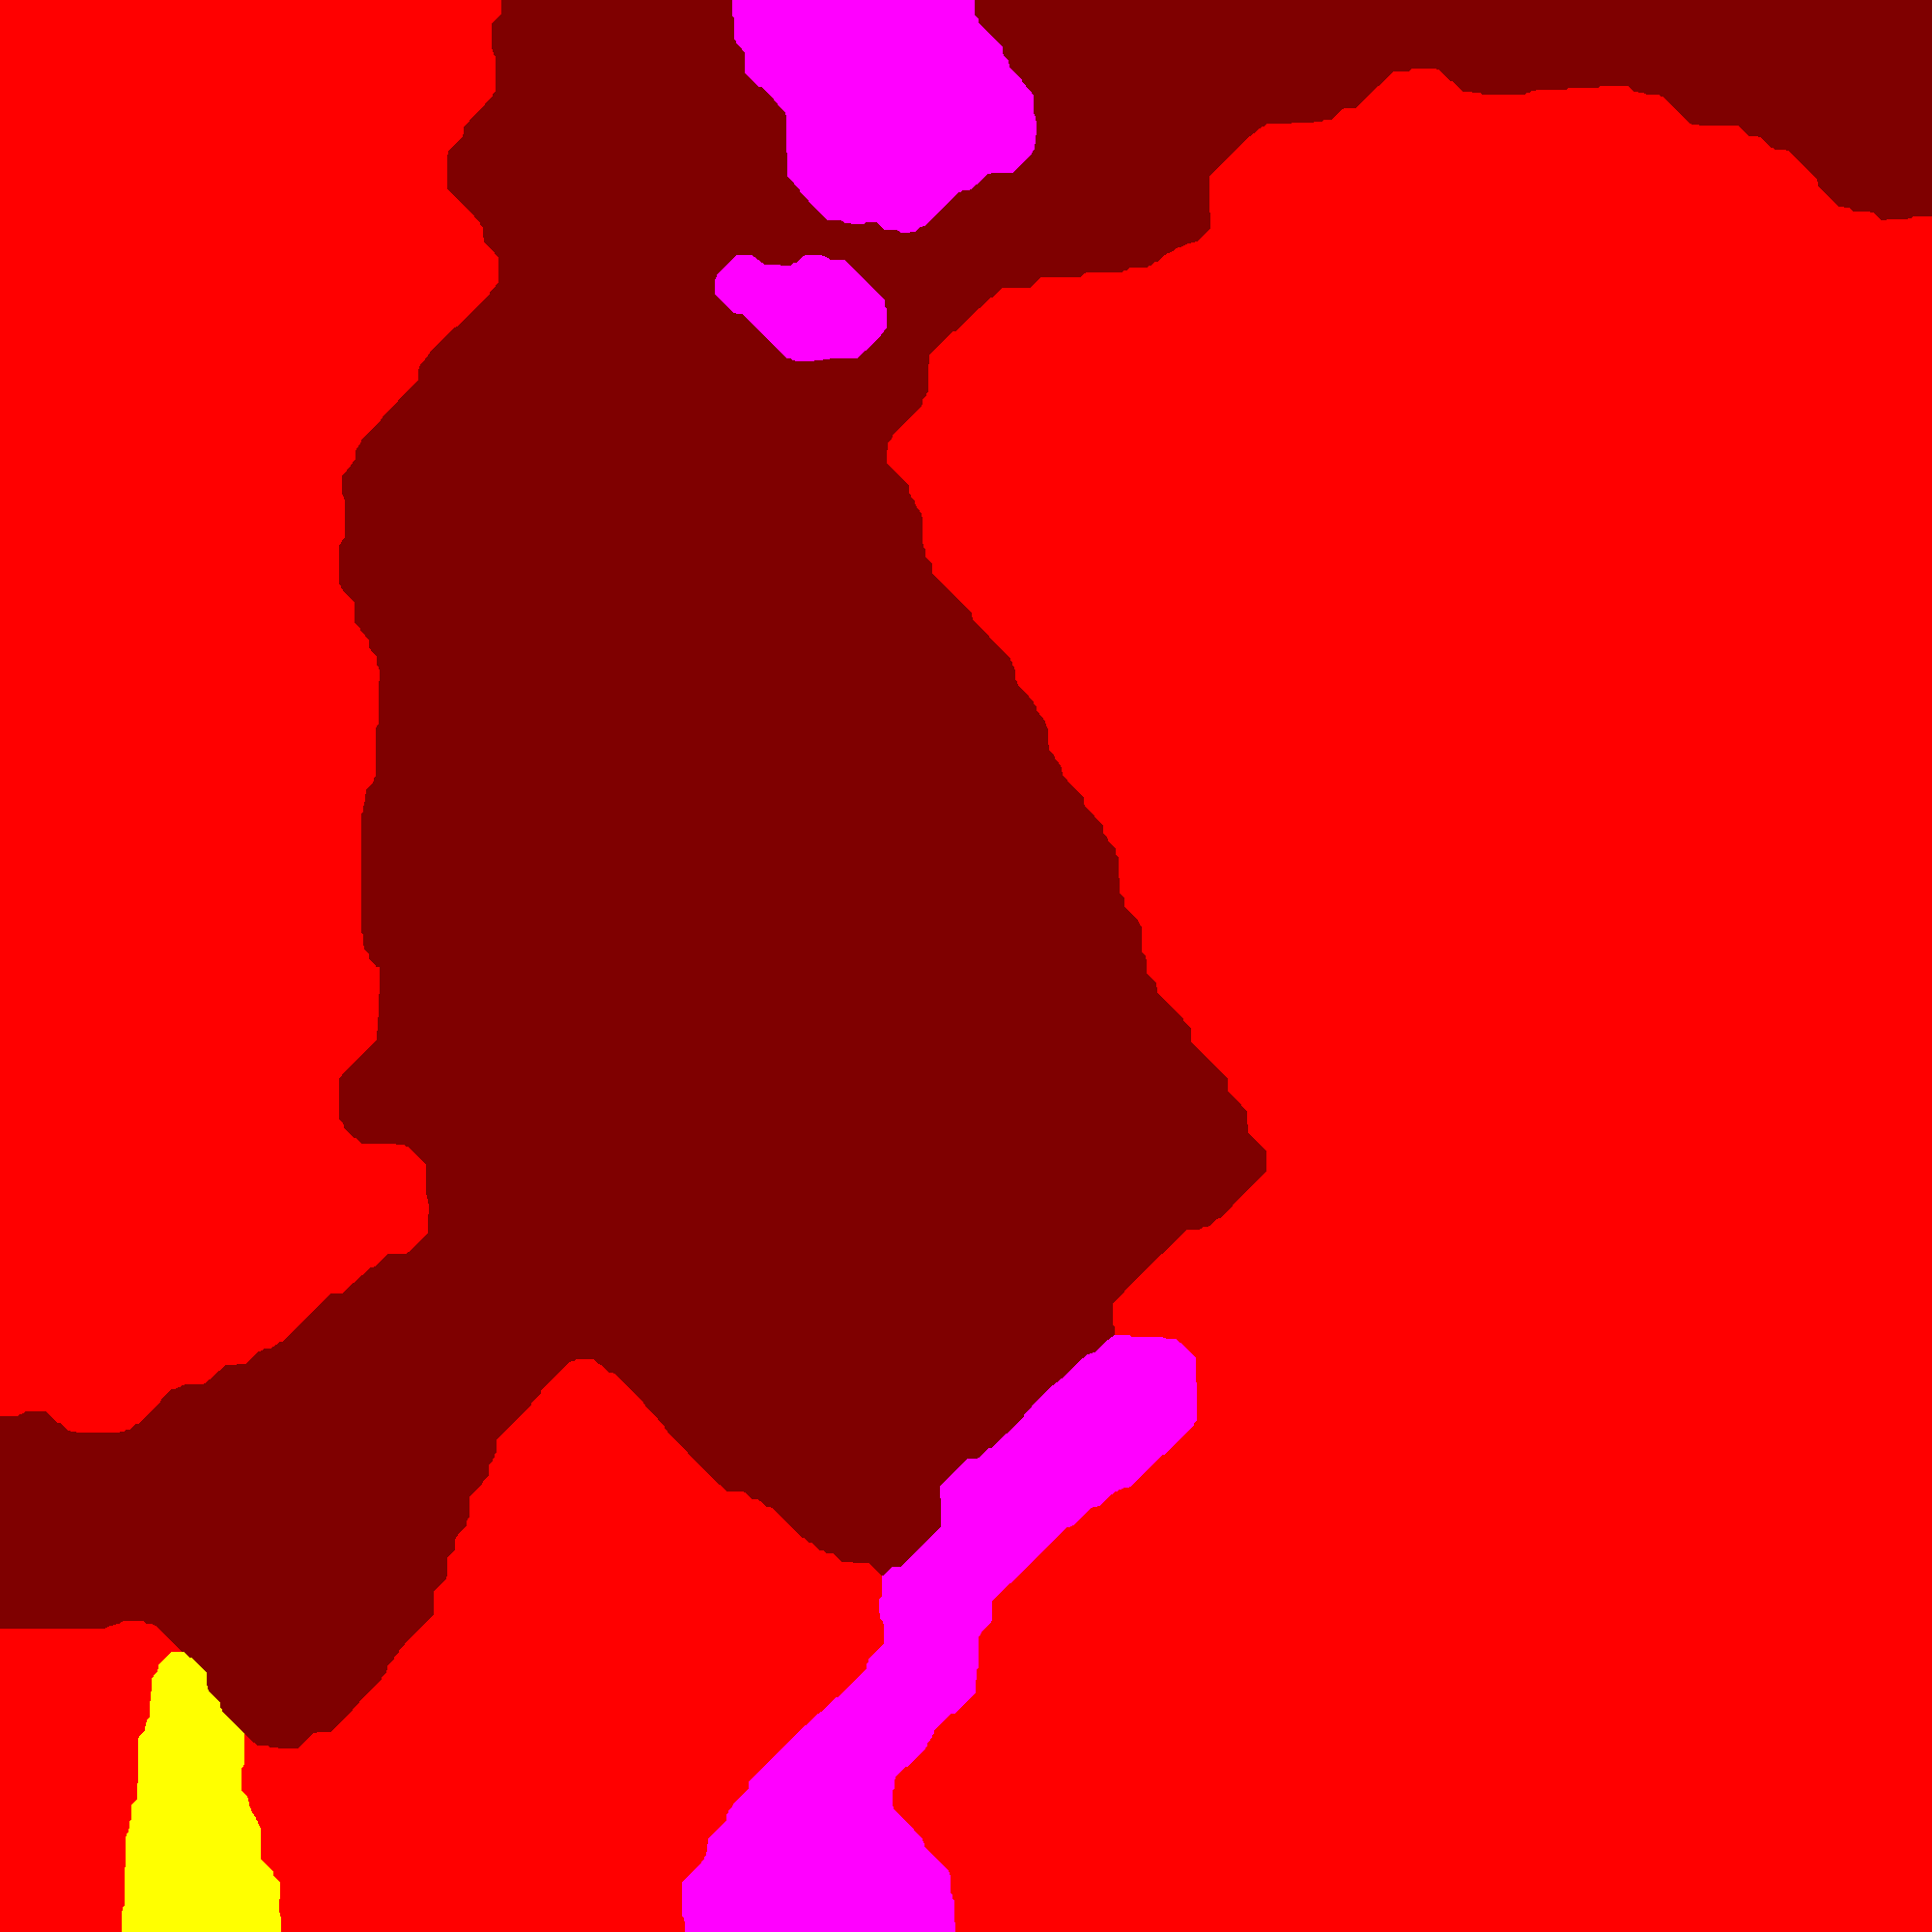
\includegraphics[width=0.3\textwidth]{Figures/C3/S3/ss1/classif_regul/quickshift/regul}
\label{subfig:C3_S3_ss1_resultsh}
}
\hspace*{0.025\textwidth}
\subfloat[SLIC.]{
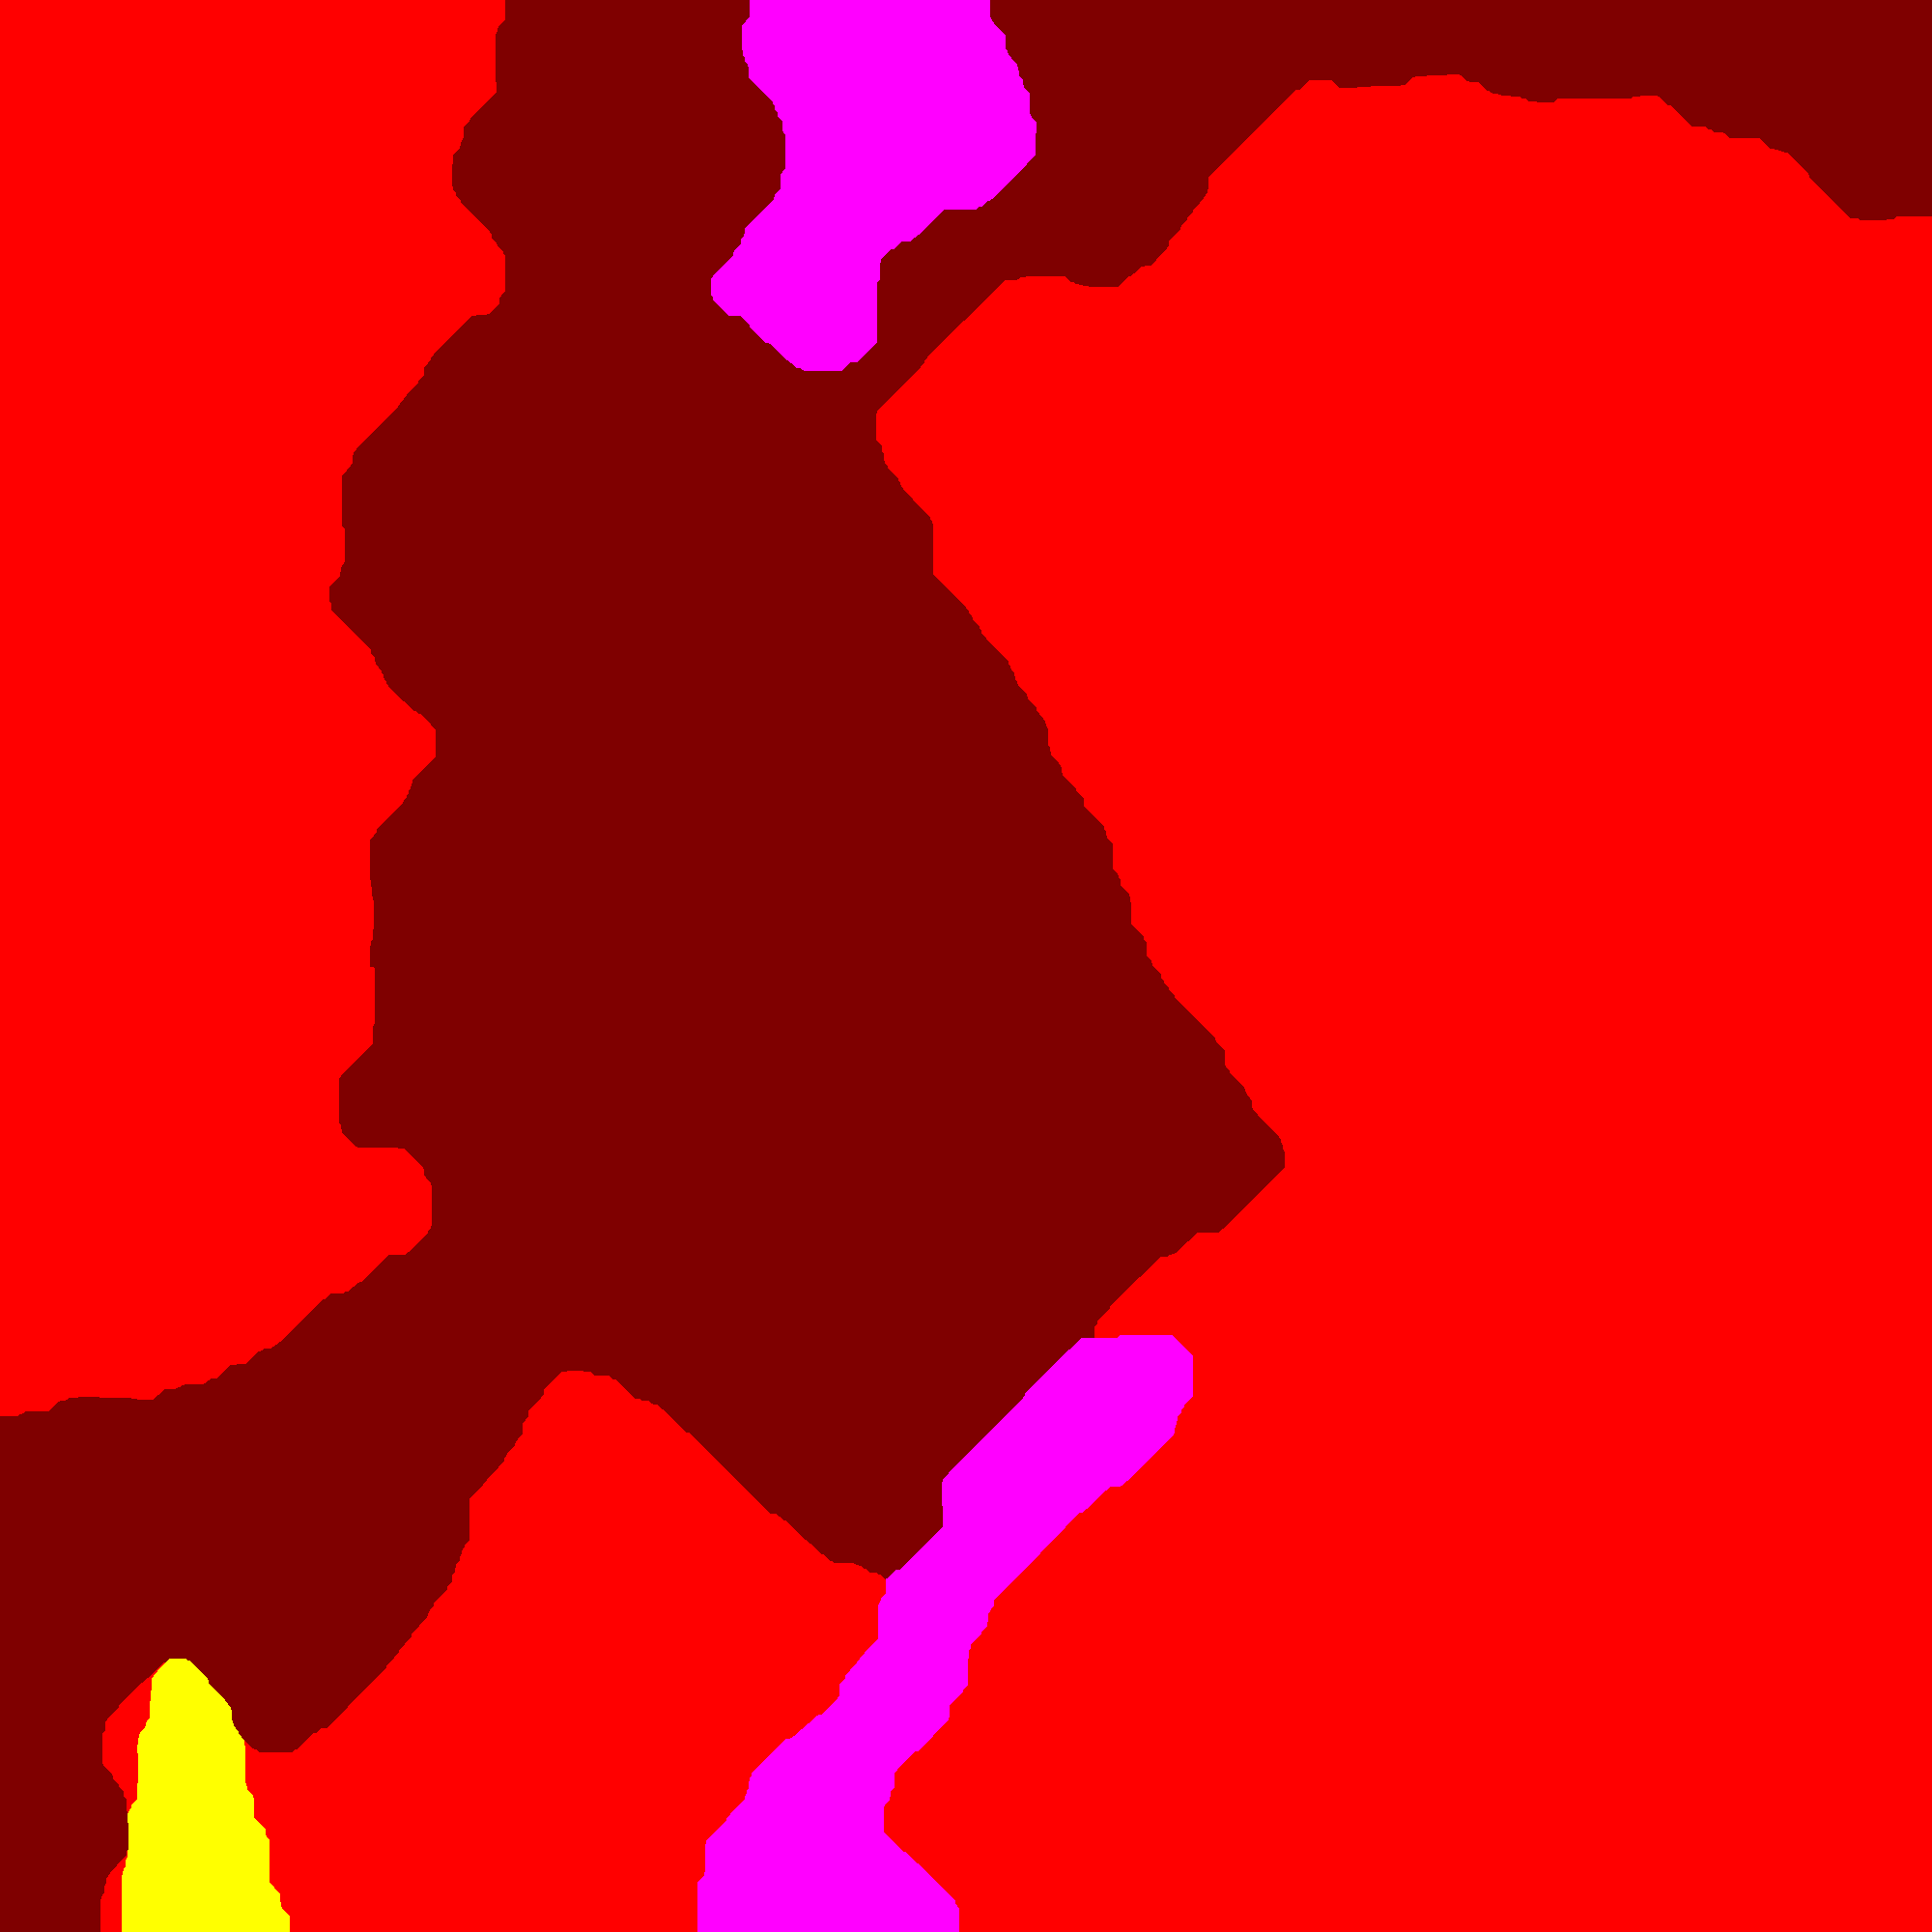
\includegraphics[width=0.3\textwidth]{Figures/C3/S3/ss1/classif_regul/SLIC/regul}
\label{subfig:C3_S3_ss1_resultsi}
}

\endgroup
\caption{Over segmentation results.}
\label{fig:C3_S3_ss1_results}
\end{center}
\end{figure}


\subsection{Feature selection}

The feature selection have been carried out for 4 main reasons.
\begin{itemize}
\item It allows to determine how many feature are needed for an optimal classification.
\item It shows the complementarity of the data (optical images and lidar).
\item It permits to understand which feature are interesting for tree species classification.
\item It reduces the computational loads and times.
\end{itemize}

\paragraph{How many features for the classification? \\}
The idea here is to obtain the number feature for an optimal classification. The idea is to run the feature selection $N$ times using all the feature. Let $a_{n,k}$ be an accuracy metric for the classification of the $n^{\text{th}}$ iteration using the $k$ ($k \in [1,K]$) best features.
The optimal number of feature $k_{opt}$ is defined as follow:
\begin{equation}
\forall k \in [1,K], \quad \sum_{n=1}^{N}a_{n,k} \leq \sum_{n=1}^{N}a_{n,k_{opt}}
\end{equation}
Here, $K=95$ and $N=50$. This experiment have been carried out on different areas, and the optimal number of feature found is $k_{opt}=20$. Thus, in all the following experiments, the classification is performed using only 20 features.

\paragraph{Complementarity of the data. \\}
Once the optimal number of features was determined, the feature selection was performed 40 times over all the test areas in order to retrieve the most relevant features. The retained attributes are presented in Figures~\ref{fig:sel_lidar},\ref{fig:sel_spectral} and~\ref{fig:sel_indices}. On average, 61\% of the selected features are derived from the spectral information and 39\% from the lidar information for a single selection (i.e., in a random selection of 20 features, 12 are derived from VHR optical images and 8 from lidar). This shows the complementarity of both remote sensing data. 

\paragraph{Features for tree species classification. \\}
For the spectral information, the features derived from the original band set are more relevant than the vegetation indices: the near-infrared derived features represent 18\% of the spectral selected features, 16\% for the red and the green, 15\% for the blue and the DVI, only 11\% for the NDVI and 10\% for the RVI. 

The most relevant statistical feature for the spectral information is the minimum (17\% of the spectral selection). The maximum (12\%), the median (11\%), the mean (11\%) and the standard deviation (10\%) are also relevant. The other statistics are selected at less than 9\% each. For more details see Figure~\ref{fig:sel_spectral} and~\ref{fig:sel_indices}. \\

For the lidar information, the most relevant feature is surprisingly the intensity, selected in each of the 40 selections (12\% of the lidar selection, 5\% of the total selection). The standard deviation (8\% of the lidar selection), the maximum (7\%) and the densities (5\% and 6\%) are also relevant. The other lidar derived features count for less than 4\% each. For more details, see Figure~\ref{fig:sel_lidar}.

\paragraph{Reduce computational loads and times. \\}
It is obvious that processing a reduced number of features (20 instead of 95) reduces the computational loads and times. Furthermore, if an optimal subset of feature is found, only the concerned features need to be computed. Thus, the feature computation step would be reduced to a minimum step by computing only the relevant features.


\pgfplotstableread[col sep=comma,header=true]{
Sel, n
{z},11
{density1},16
{density2},20
{planarity},11
{scatter},6
{min},10
{max},23
{mean},7
{median},9
{standard deviation},24
{medADmed},14
{meanADmed},14
{skewness},4
{kurtosis},7
{10th percentile},8
{20th percentile},9
{30th percentile},10
{40th percentile},9
{50th percentile},7
{60th percentile},11
{70th percentile},12
{80th percentile},8
{90th percentile},11
{95th percentile},8
{intensity},40
}\datalidar

\begin{figure}[htbp]
\begin{center}
    \begin{tikzpicture}
    {
        \begin{axis}[    
            width=0.75\textwidth,
            xbar,                                 
            xtick={0,5,10,...,45},    
            xmin=0,
            xmax=45,       
            grid=major,
            nodes near coords, nodes near coords align={horizontal},
            symbolic y coords={intensity, 95th percentile, 90th percentile, 80th percentile, 70th percentile, 60th percentile, 50th percentile, 40th percentile, 30th percentile, 20th percentile, 10th percentile, kurtosis, skewness, meanADmed, medADmed, standard deviation, median, mean, max, min, scatter, planarity, density2, density1, z},
            ylabel={Features},
            ytick=data,
            xlabel={Number of selections},
            y label style={at={(-0.33,0.5)}},
            enlarge x limits={abs=0},
            y=0.025\textheight,
            reverse legend
        ]
        \addplot[color=black, fill=black!80!white] table [x=n, y=Sel] {\datalidar};
        \end{axis}
    }
    \end{tikzpicture}
\caption{Result of the feature selection for the lidar features over 40 trials of 20 optimal features.}
\label{fig:sel_lidar}
\end{center}
\end{figure}

%\pgfplotstableread[col sep=comma,header=true]{
%Sel, n
%{z},11
%{density1},16
%{density2},20
%{planarity},11
%{scatter},6
%{min},10
%{max},23
%{mean},7
%{median},9
%{standard deviation},24
%{medADmed},14
%{meanADmed},14
%{skewness},4
%{kurtosis},7
%{10$^{\text{th}}$percentile},8
%{20$^{\text{th}}$percentile},9
%{30$^{\text{th}}$percentile},10
%{40$^{\text{th}}$percentile},9
%{50$^{\text{th}}$percentile},7
%{60$^{\text{th}}$percentile},11
%{70$^{\text{th}}$percentile},12
%{80$^{\text{th}}$percentile},8
%{90$^{\text{th}}$percentile},11
%{95$^{\text{th}}$percentile},8
%{intensity},40
%}\datalidar
%
%\begin{figure}[htbp]
%\begin{center}
%    \begin{tikzpicture}
%    {
%        \begin{axis}[    
%            width=0.75\textwidth,
%            xbar,                                 
%            xtick={0,5,10,...,45},    
%            xmin=0,
%            xmax=45,       
%            grid=major,
%            nodes near coords, nodes near coords align={horizontal},
%            symbolic y coords={intensity, 95$^{\text{th}}$percentile, 90$^{\text{th}}$percentile, 80$^{\text{th}}$percentile, 70$^{\text{th}}$percentile, 60$^{\text{th}}$percentile, 50$^{\text{th}}$percentile, 40$^{\text{th}}$percentile, 30$^{\text{th}}$percentile, 20$^{\text{th}}$percentile, 10$^{\text{th}}$percentile, kurtosis, skewness, meanADmed, medADmed, standard deviation, median, mean, max, min, scatter, planarity, density2, density1, z},
%            ylabel={Features},
%            ytick=data,
%            xlabel={Number of selections},
%            y label style={at={(-0.33,0.5)}},
%            enlarge x limits={abs=0},
%            y=0.025\textheight,
%            reverse legend
%        ]
%        \addplot[color=black, fill=black!80!white] table [x=n, y=Sel] {\datalidar};
%        \end{axis}
%    }
%    \end{tikzpicture}
%\caption{Result of the feature selection for the lidar features over 40 trials of 20 optimal features.}
%\label{fig:sel_lidar}
%\end{center}
%\end{figure}
%
\pgfplotstableread[col sep=comma,header=true]{
Sel, R, G, B, NIR
Band,8,5,8,6
min,15,15,11,18
max,15,6,8,14
mean,8,11,13,13
median,7,9,7,9
standard deviation,5,6,9,6
meanADmed,6,7,7,3
meanADmean,4,3,5,9
medADmed,8,6,5,6
medADmean,4,6,4,4
}\dataspectral

\begin{figure} [htbp]%
\begin{center}
    \begin{tikzpicture}     
        \begin{axis}[    
            width=0.75\textwidth,
            xbar,                                 
            xtick={0,5,10,...,20},    
            xmin=0,
            xmax=20,       
            grid=major,
            nodes near coords, nodes near coords align={horizontal},
            symbolic y coords={medADmean,medADmed,meanADmean,meanADmed,standard deviation,median,mean,max,min,Band},
            ylabel={Features},
            ytick=data,
            xlabel={Number of selections},
            y label style={at={(-0.33,0.5)}},
            enlarge x limits={abs=0},
            y=0.09\textheight,
            reverse legend,
        ]
        \addplot[color=black, fill=gray!80!white] table [x=NIR, y=Sel] {\dataspectral};
        \addplot[color=black, fill=blue!80!white] table [x=B, y=Sel] {\dataspectral};  
        \addplot[color=black, fill=green!80!white] table [x=G, y=Sel] {\dataspectral};
        \addplot[color=black, fill=red!80!white] table [x=R, y=Sel] {\dataspectral};
        \legend{NIR band, Blue band, Green band, Red band}
        \end{axis}
    \end{tikzpicture}
\caption{Result of the feature selection for the spectral features over 40 trials of 20 optimal features.}
\label{fig:sel_spectral}
\end{center}
\end{figure}

\pgfplotstableread[col sep=comma,header=true]{
Sel, NDVI, DVI, RVI
Band,6,3,2
min,7,11,8
max,6,5,5
mean,2,3,3
median,6,11,6
standard deviation,8,11,5
meanADmed,9,4,6
meanADmean,5,3,4
medADmed,3,10,6
medADmean,3,7,5
}\dataindices

\begin{figure} [htbp]%
\begin{center}
    \begin{tikzpicture}     
        \begin{axis}[    
            width=0.75\textwidth,
            xbar,                                 
            xtick={0,5,10,...,15},    
            xmin=0,
            xmax=15,       
            grid=major,
            nodes near coords, nodes near coords align={horizontal},
            symbolic y coords={medADmean,medADmed,meanADmean,meanADmed,standard deviation,median,mean,max,min,Band},
            ylabel={Features},
            ytick=data,
            xlabel={Number of selections},
            y label style={at={(-0.33,0.5)}},
            enlarge x limits={abs=0},
            y=0.075\textheight,
            reverse legend,
        ]
        \addplot[color=black, fill=i2!80!white] table [x=RVI, y=Sel] {\dataindices};  
        \addplot[color=black, fill=i1!80!white] table [x=DVI, y=Sel] {\dataindices};
        \addplot[color=black, fill=i0!80!white] table [x=NDVI, y=Sel] {\dataindices};
        \legend{RVI, DVI, NDVI}
        \end{axis}
    \end{tikzpicture}
\end{center}
\caption{Result of the feature selection for the vegetation indices features over 40 trials of 20 optimal features.}
\label{fig:sel_indices}
\end{figure}


\subsection{Classification}
The classification is composed of two steps, the selection of training samples and the classification itself.
The classification is mainly performed using standard RF classifier \citep{opencv}. Tests have also been conducted using a SVM classifier with RBF kernel \citep{vapnik2013nature}. The classification can be impacted by two factors:
\begin{itemize}
\item The selection or non-selection of training pixels.
\item The object-based or pixel-based analysis.
\end{itemize}

\paragraph{Pixel-based classification versus object-based classification. \\}
The results of pixel-based and object-based classification is presented in Figure~\ref{fig:C3_S3_ss3_po}. The corresponding confusion matrices and accuracy metrics are presented in Tables~\ref{table:C3_S3_ss3_classif_pixel} and~\ref{table:C3_S3_ss3_classif_PFF}.

\begin{figure}[htbp]
\begin{center}
\begingroup
\captionsetup[subfigure]{width=0.425\textwidth}
\subfloat[IRC VHR optical image.]{
\includegraphics[width=0.45\textwidth]{Figures/C3/S3/ss3/IRC}
\label{subfig:C3_S3_ss3_poa}
}
\hspace*{0.025\textwidth}
\subfloat[Forest LC.]{
\includegraphics[width=0.45\textwidth]{Figures/C3/S3/ss3/BD}
\label{subfig:C3_S3_ss3_pob}
}
\\
\subfloat[Pixel-based classification (overall accuracy: 70.48\%, $\kappa$: 0.50).]{
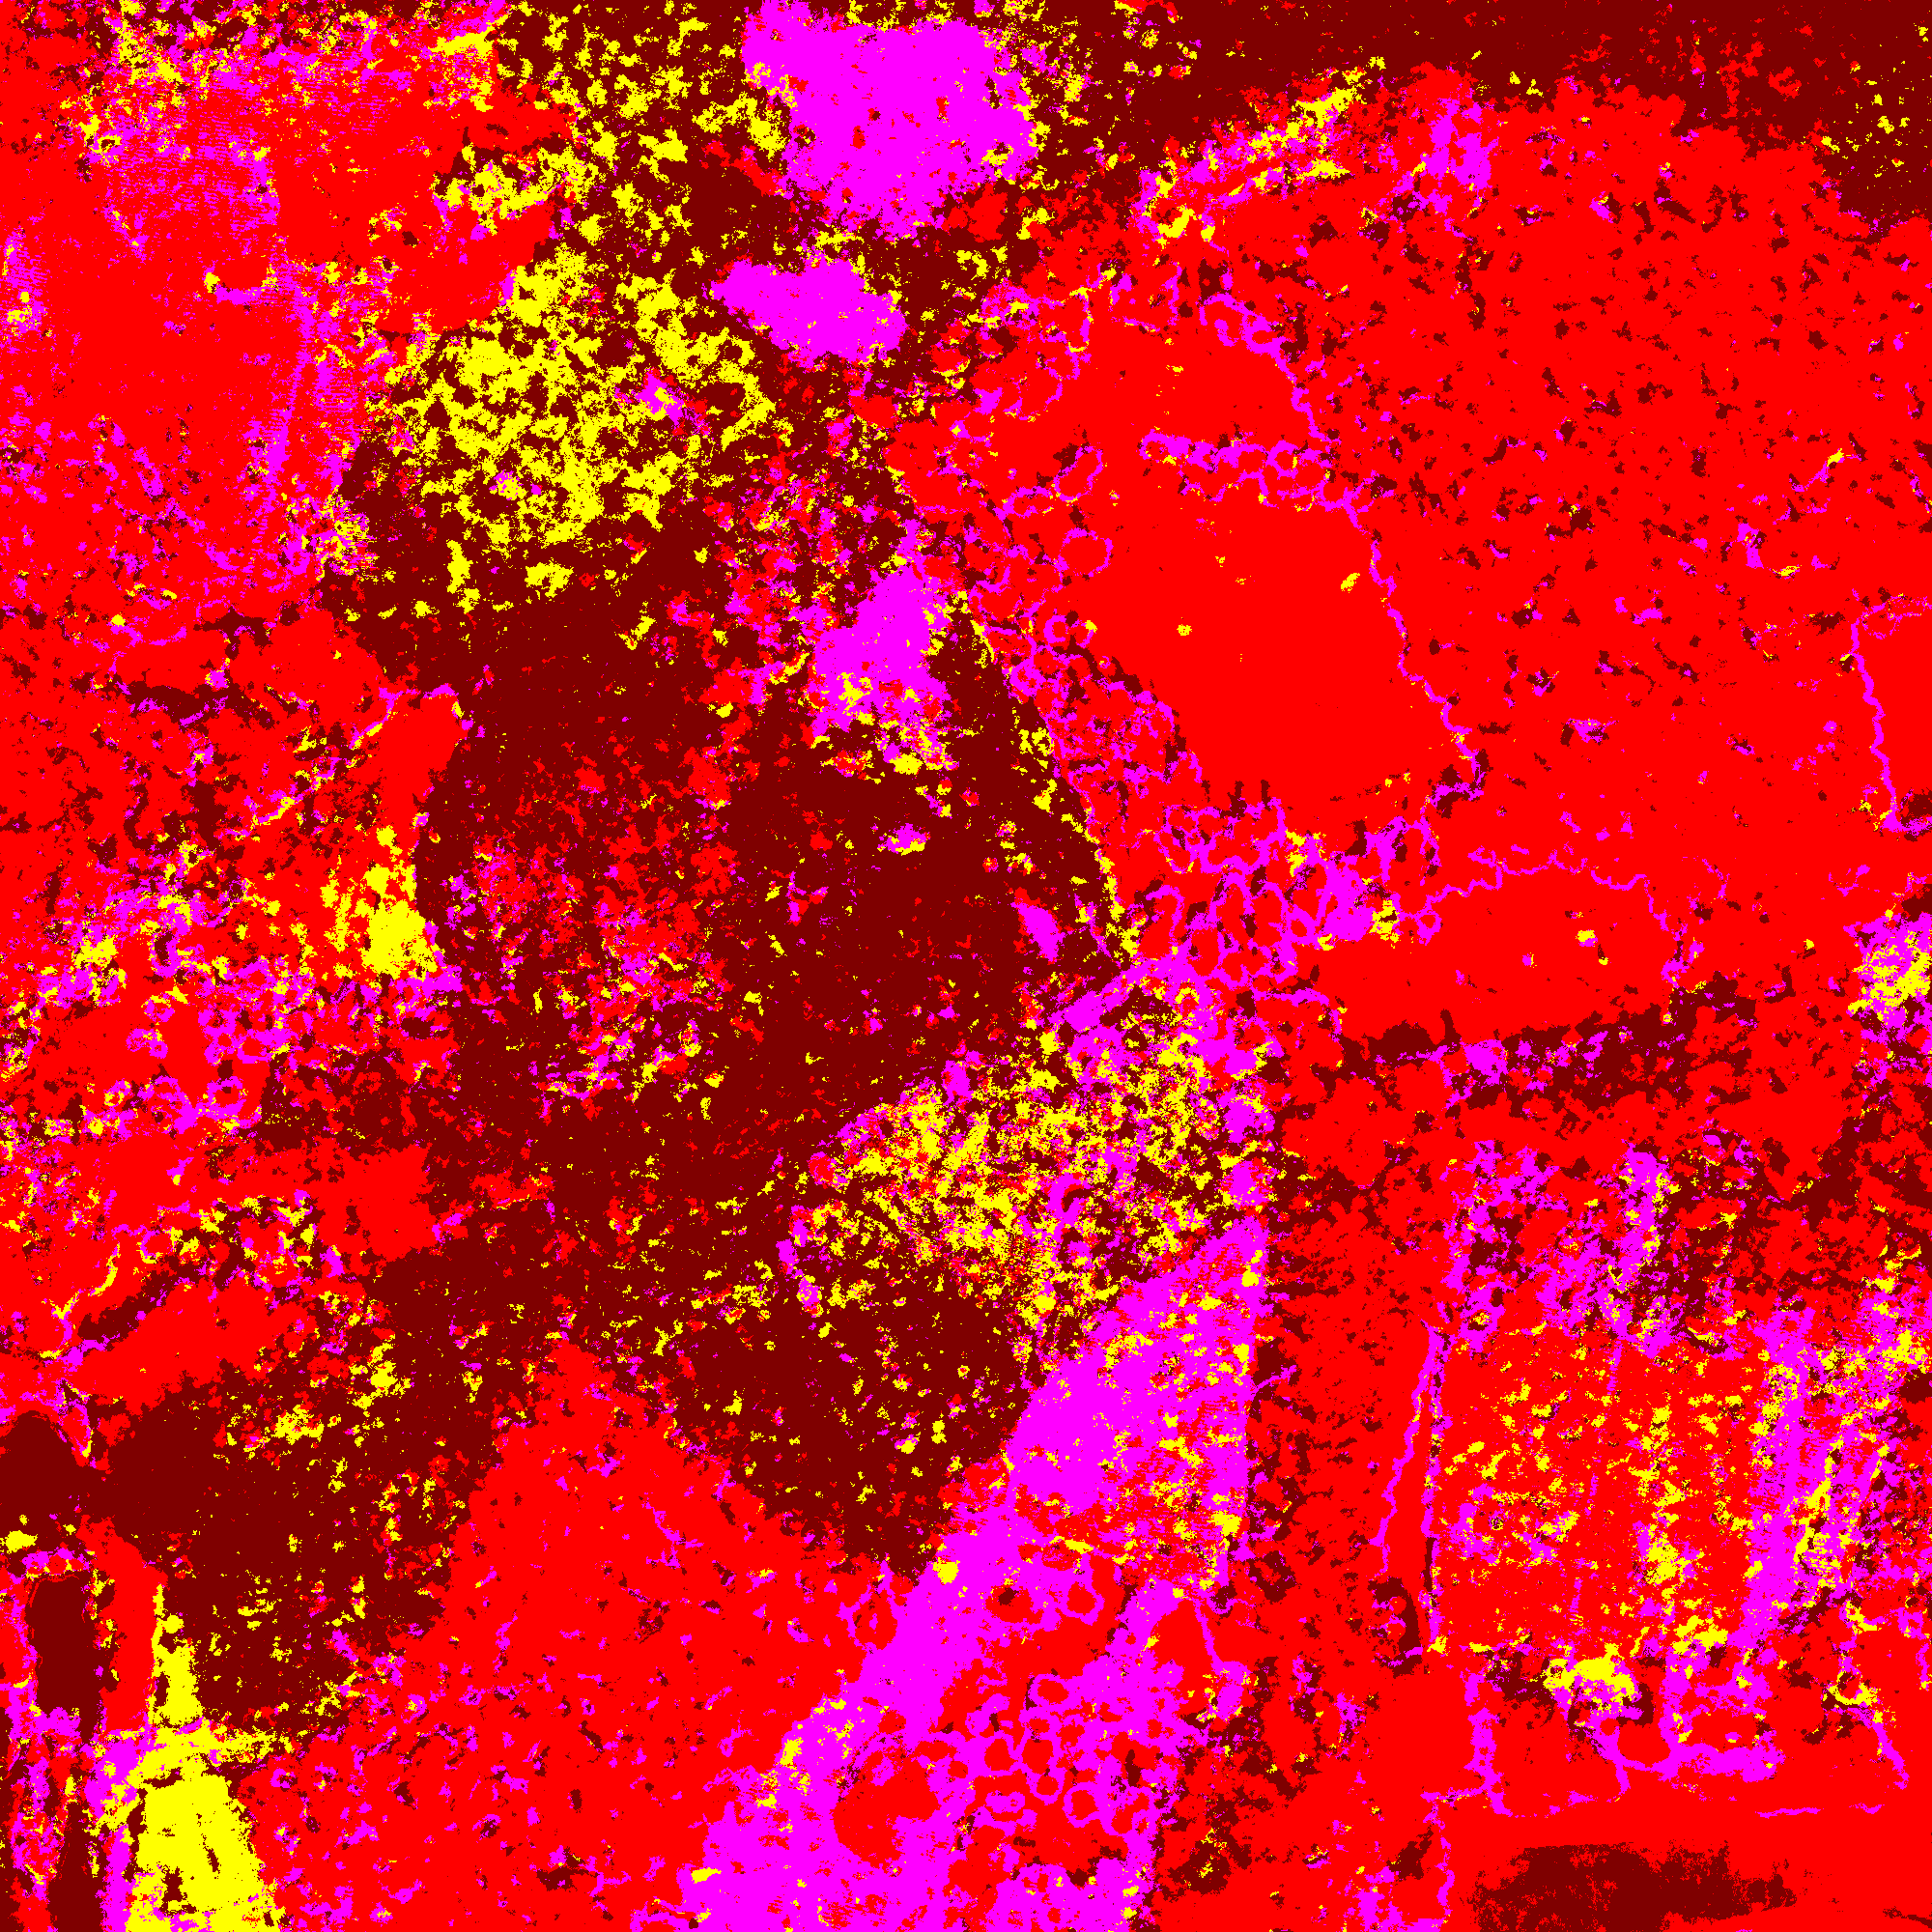
\includegraphics[width=0.45\textwidth]{Figures/C3/S3/ss3/classif_pixel}
\label{subfig:C3_S3_ss3_poc}
}
\hspace*{0.025\textwidth}
\subfloat[Object-based classification (PFF) (overall accuracy: 93.14\%, $\kappa$: 0.86).]{
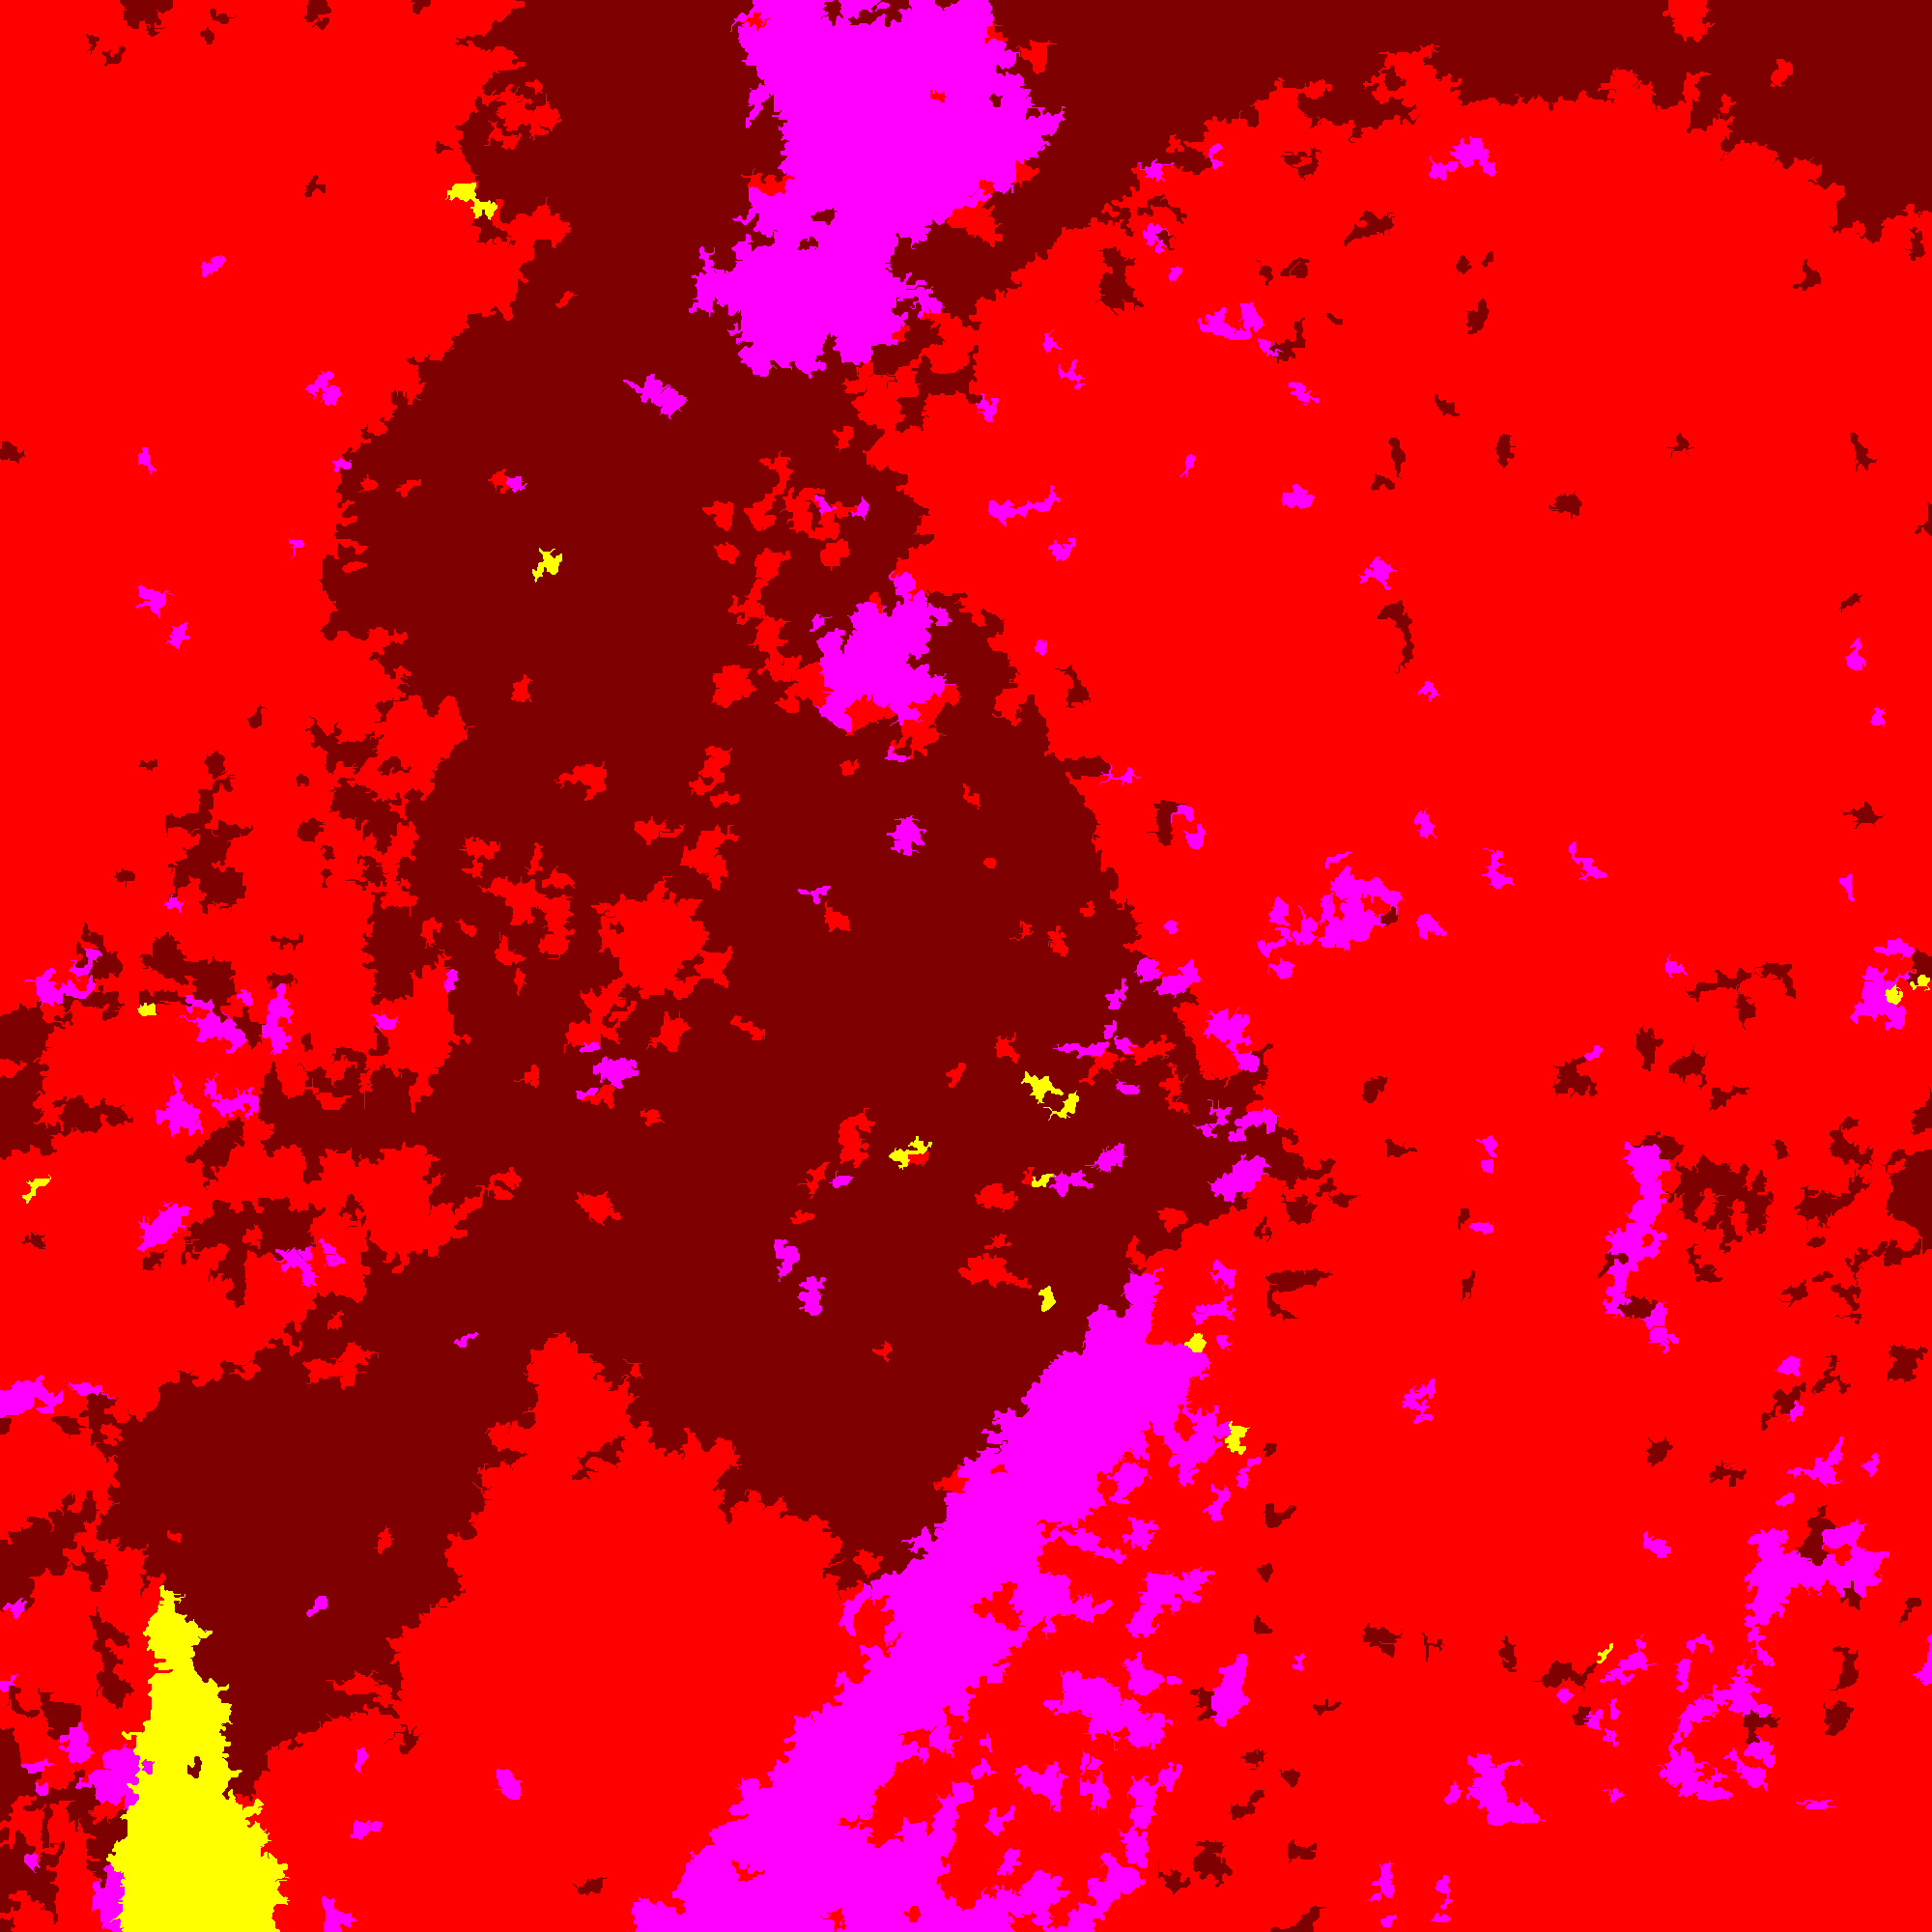
\includegraphics[width=0.45\textwidth]{Figures/C3/S3/ss3/classif_PFF}
\label{subfig:C3_S3_ss3_pod}
}
\endgroup
\caption{Classification results; pixel-based versus object-based.}
\label{fig:C3_S3_ss3_po}
\end{center}
\end{figure}

The pixel-based classification (Figure~\ref{subfig:C3_S3_ss3_poc}) appears more noisy than the object-based classification (Figure~\ref{subfig:C3_S3_ss3_pod}). However, the pixel-based classification already provide good discrimination results. Conversely, even if the object are roughly extracted (no specific attention is paid to the relevance of the extracted objects), the object-based classification produces more spatially consistent labels. Such results impacts the final output (see Figure~\ref{fig:C3_S3_ss3_rpo} and Tables~\ref{table:C3_S3_ss3_regul_pixel} and~\ref{table:C3_S3_ss3_regul_PFF}).

\begin{figure}[htbp]
\begin{center}
\begingroup
\captionsetup[subfigure]{width=0.425\textwidth}
\subfloat[Regularization using pixel-based classification (overall accuracy: 91.94\%, $\kappa$: 0.85).]{
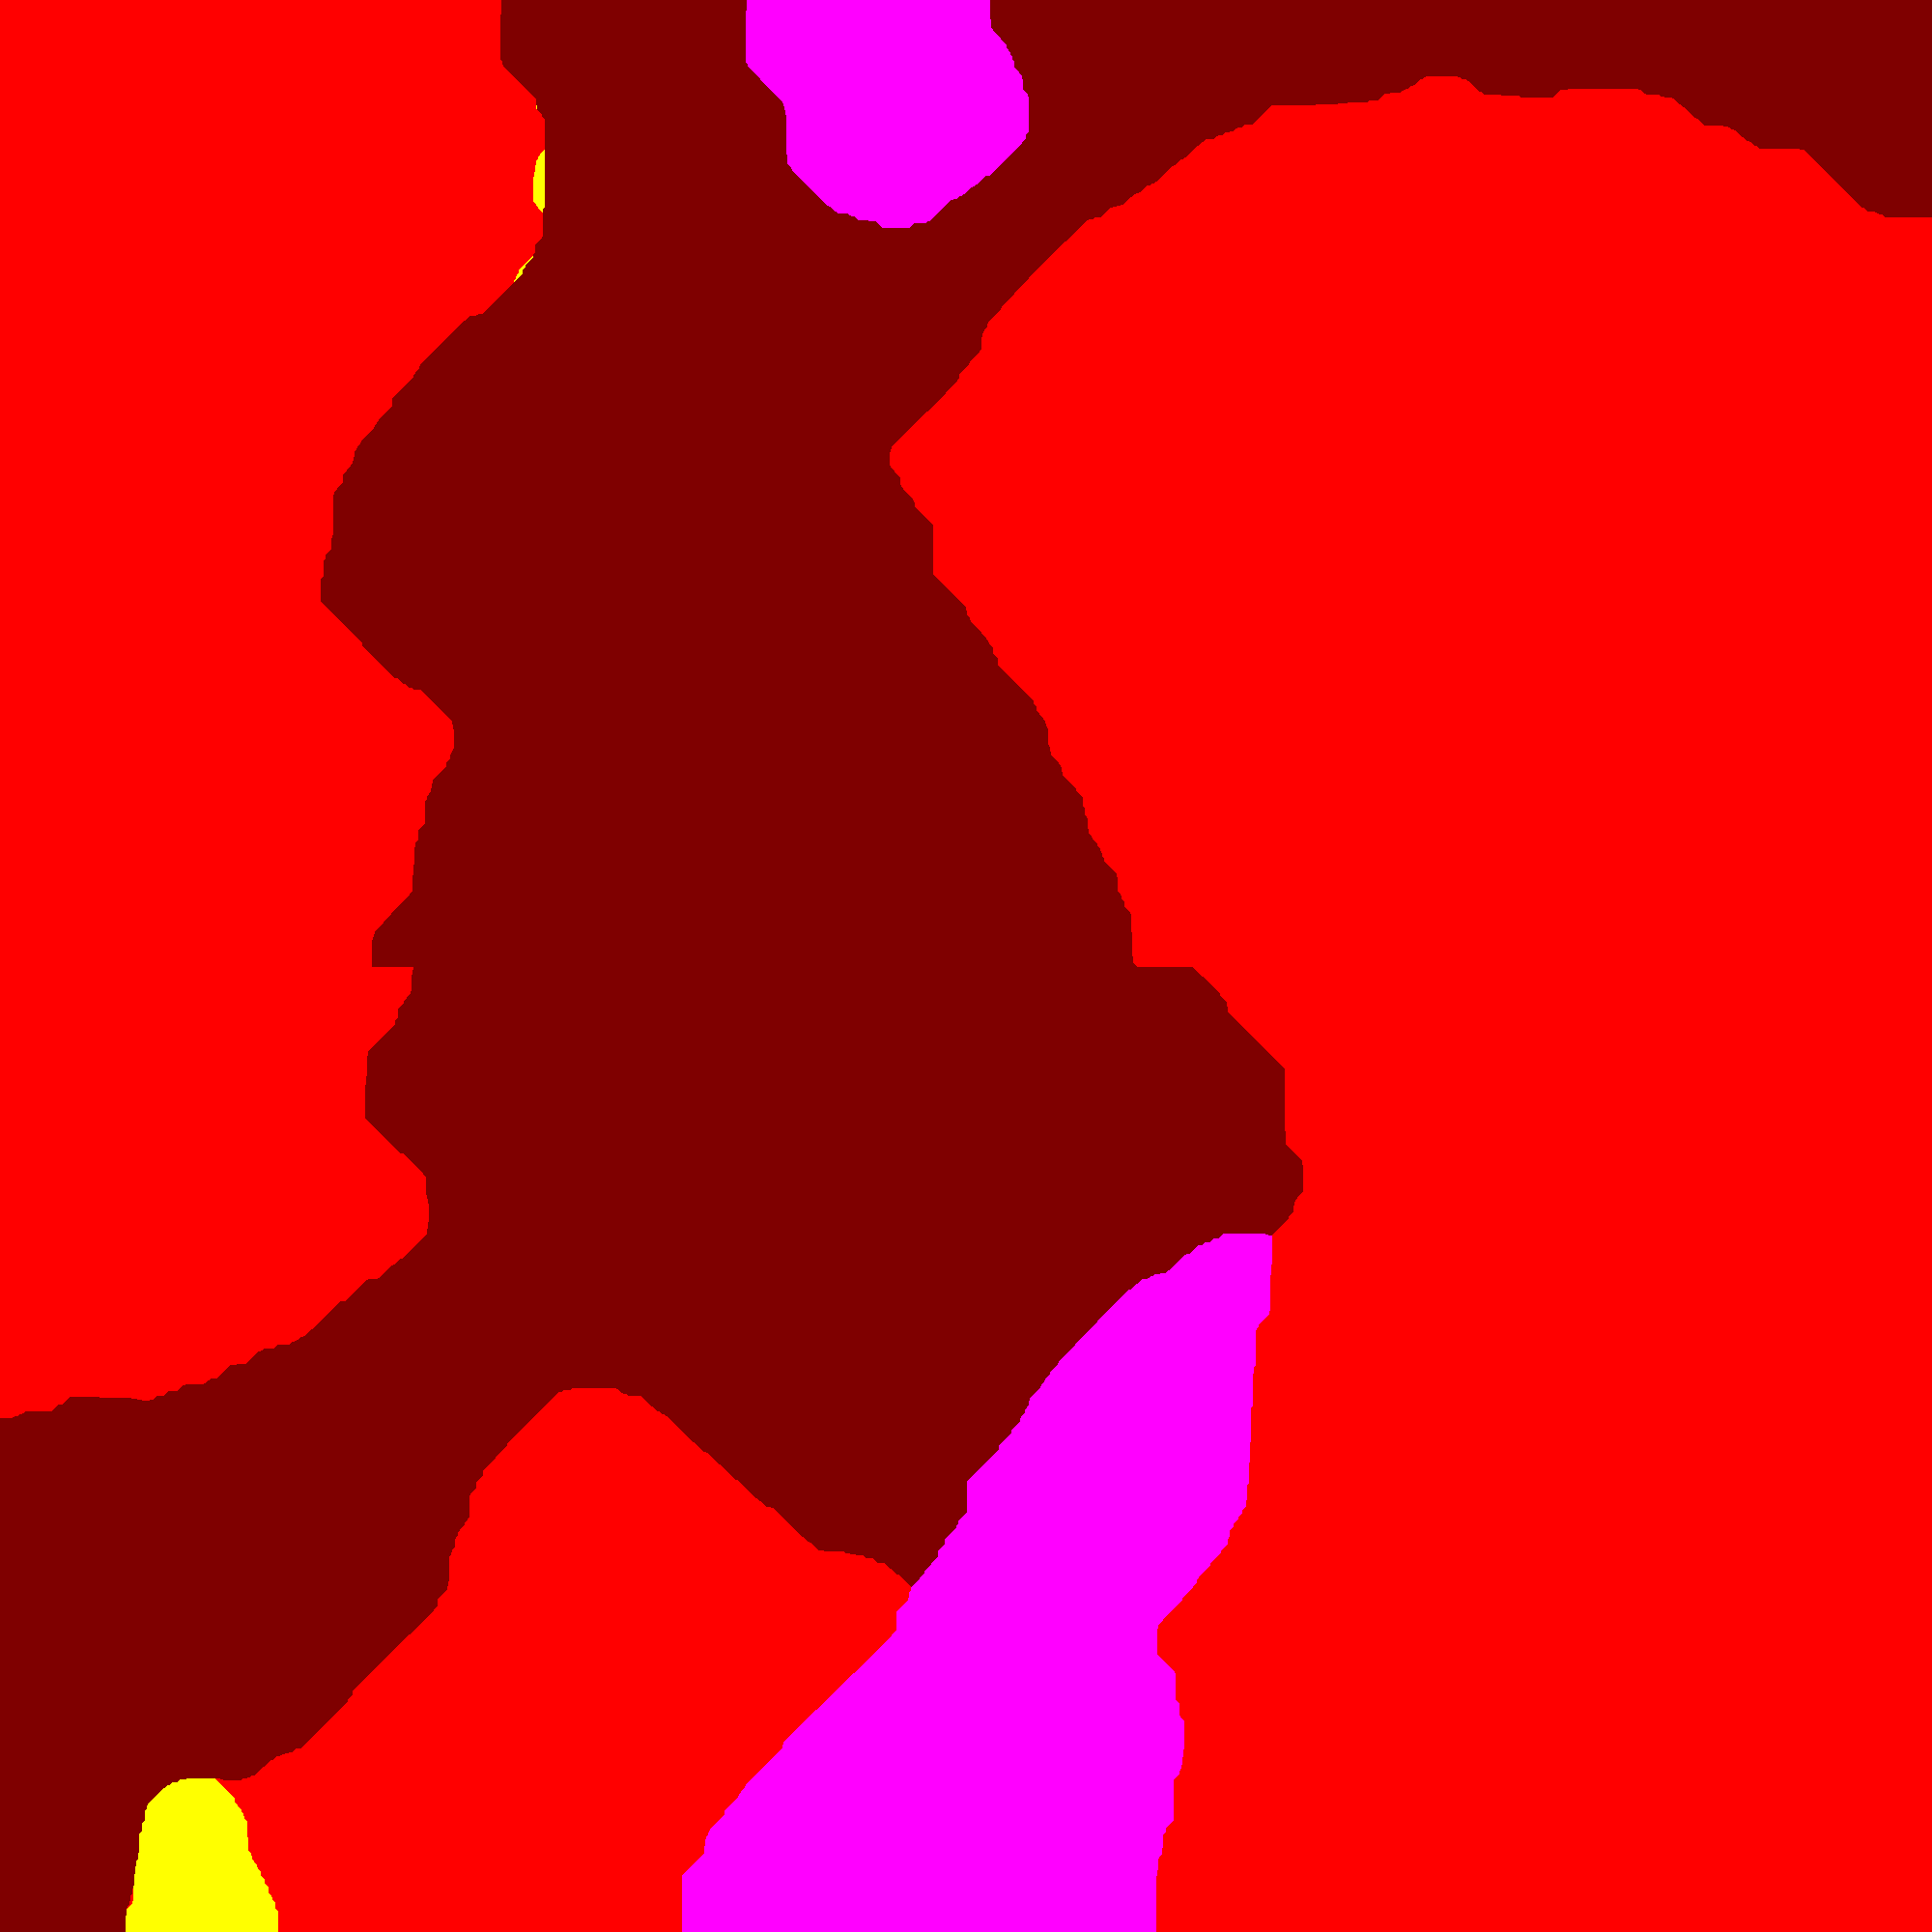
\includegraphics[width=0.45\textwidth]{Figures/C3/S3/ss3/regul_pixel}
\label{subfig:C3_S3_ss3_rpoa}
}
\hspace*{0.025\textwidth}
\subfloat[Regularization using object-based classification (PFF) (overall accuracy: 97.44\%, $\kappa$: 0.95).]{
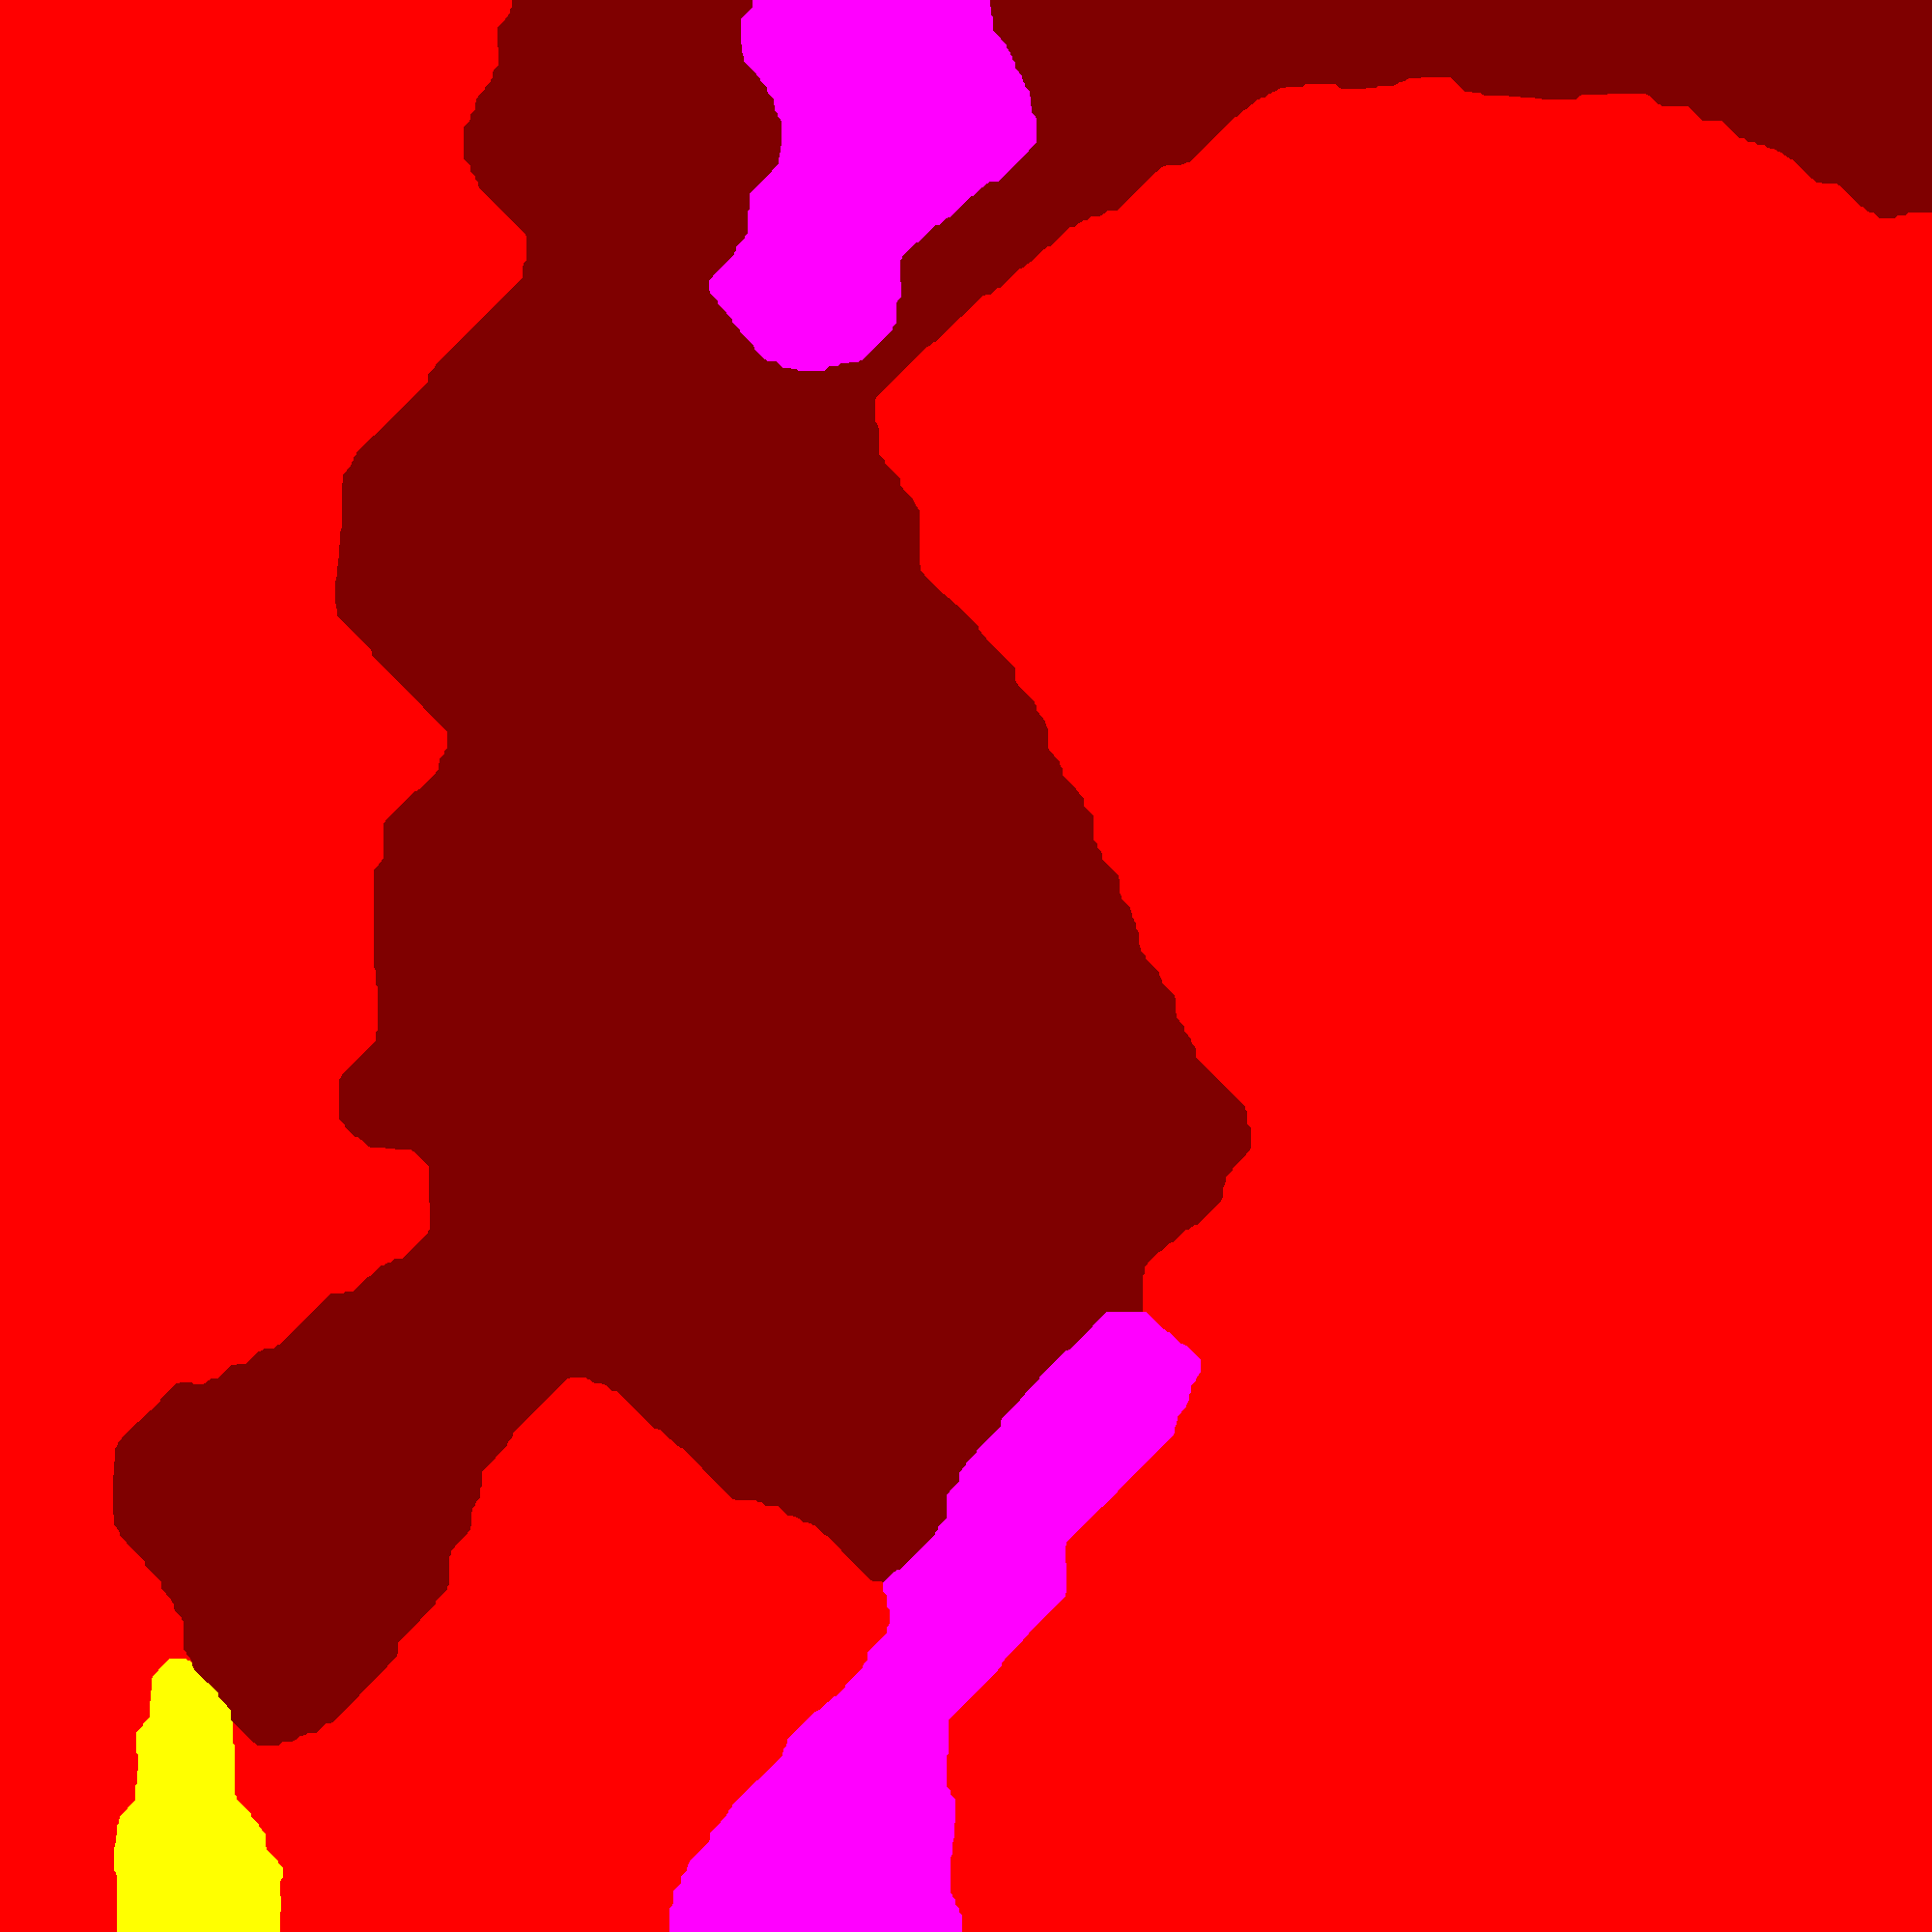
\includegraphics[width=0.45\textwidth]{Figures/C3/S3/ss3/regul_PFF}
\label{subfig:C3_S3_ss3_rpob}
}
\endgroup
\caption{Regularization results; pixel-based classification versus object-based classification.}
\label{fig:C3_S3_ss3_rpo}
\end{center}
\end{figure}

\paragraph{Training set design. \\}

The selection of the training pixels is an important step for the classification. It is a two sided problem:
\begin{itemize}
\item If the selected pixels are randomly taken from the polygons of the forest LC, some might not correspond to the target class, leading to confusion in the final classification.
\item If the pixels are selected using a too discriminative criteria, the variability of the target class will not be taken into account, also leading to confusion in the final classification.
\end{itemize}

The Figure~\ref{fig:C3_S3_ss3_sel} shows the pixels that have been selected by the k-mean algorithm for the training. Most of the pixel from the forest LC are retained. However, the pixels that are excluded from the training are visually relevant. Indeed, they mostly correspond to:
\begin{itemize}
\item Shadows from the optical images,
\item gaps in the canopy (retrieved from the lidar data),
\item pixels that are visually different from the other pixels of the considered class (i.e. other species).
\end{itemize}

The selection of training pixels is beneficial since it allows to remove the obviously irrelevant pixels from the training set while maintaining a certain variability within classes.

\begin{figure}[htbp]
\begin{center}
\begingroup
\captionsetup[subfigure]{width=0.45\textwidth}
\subfloat[RGB VHR optical image.]{
\includegraphics[width=0.45\textwidth]{Figures/C3/S3/ss3/RGB}
\label{subfig:C3_S3_ss_sela}
}
\hspace*{0.025\textwidth}
\subfloat[nDSM.]{
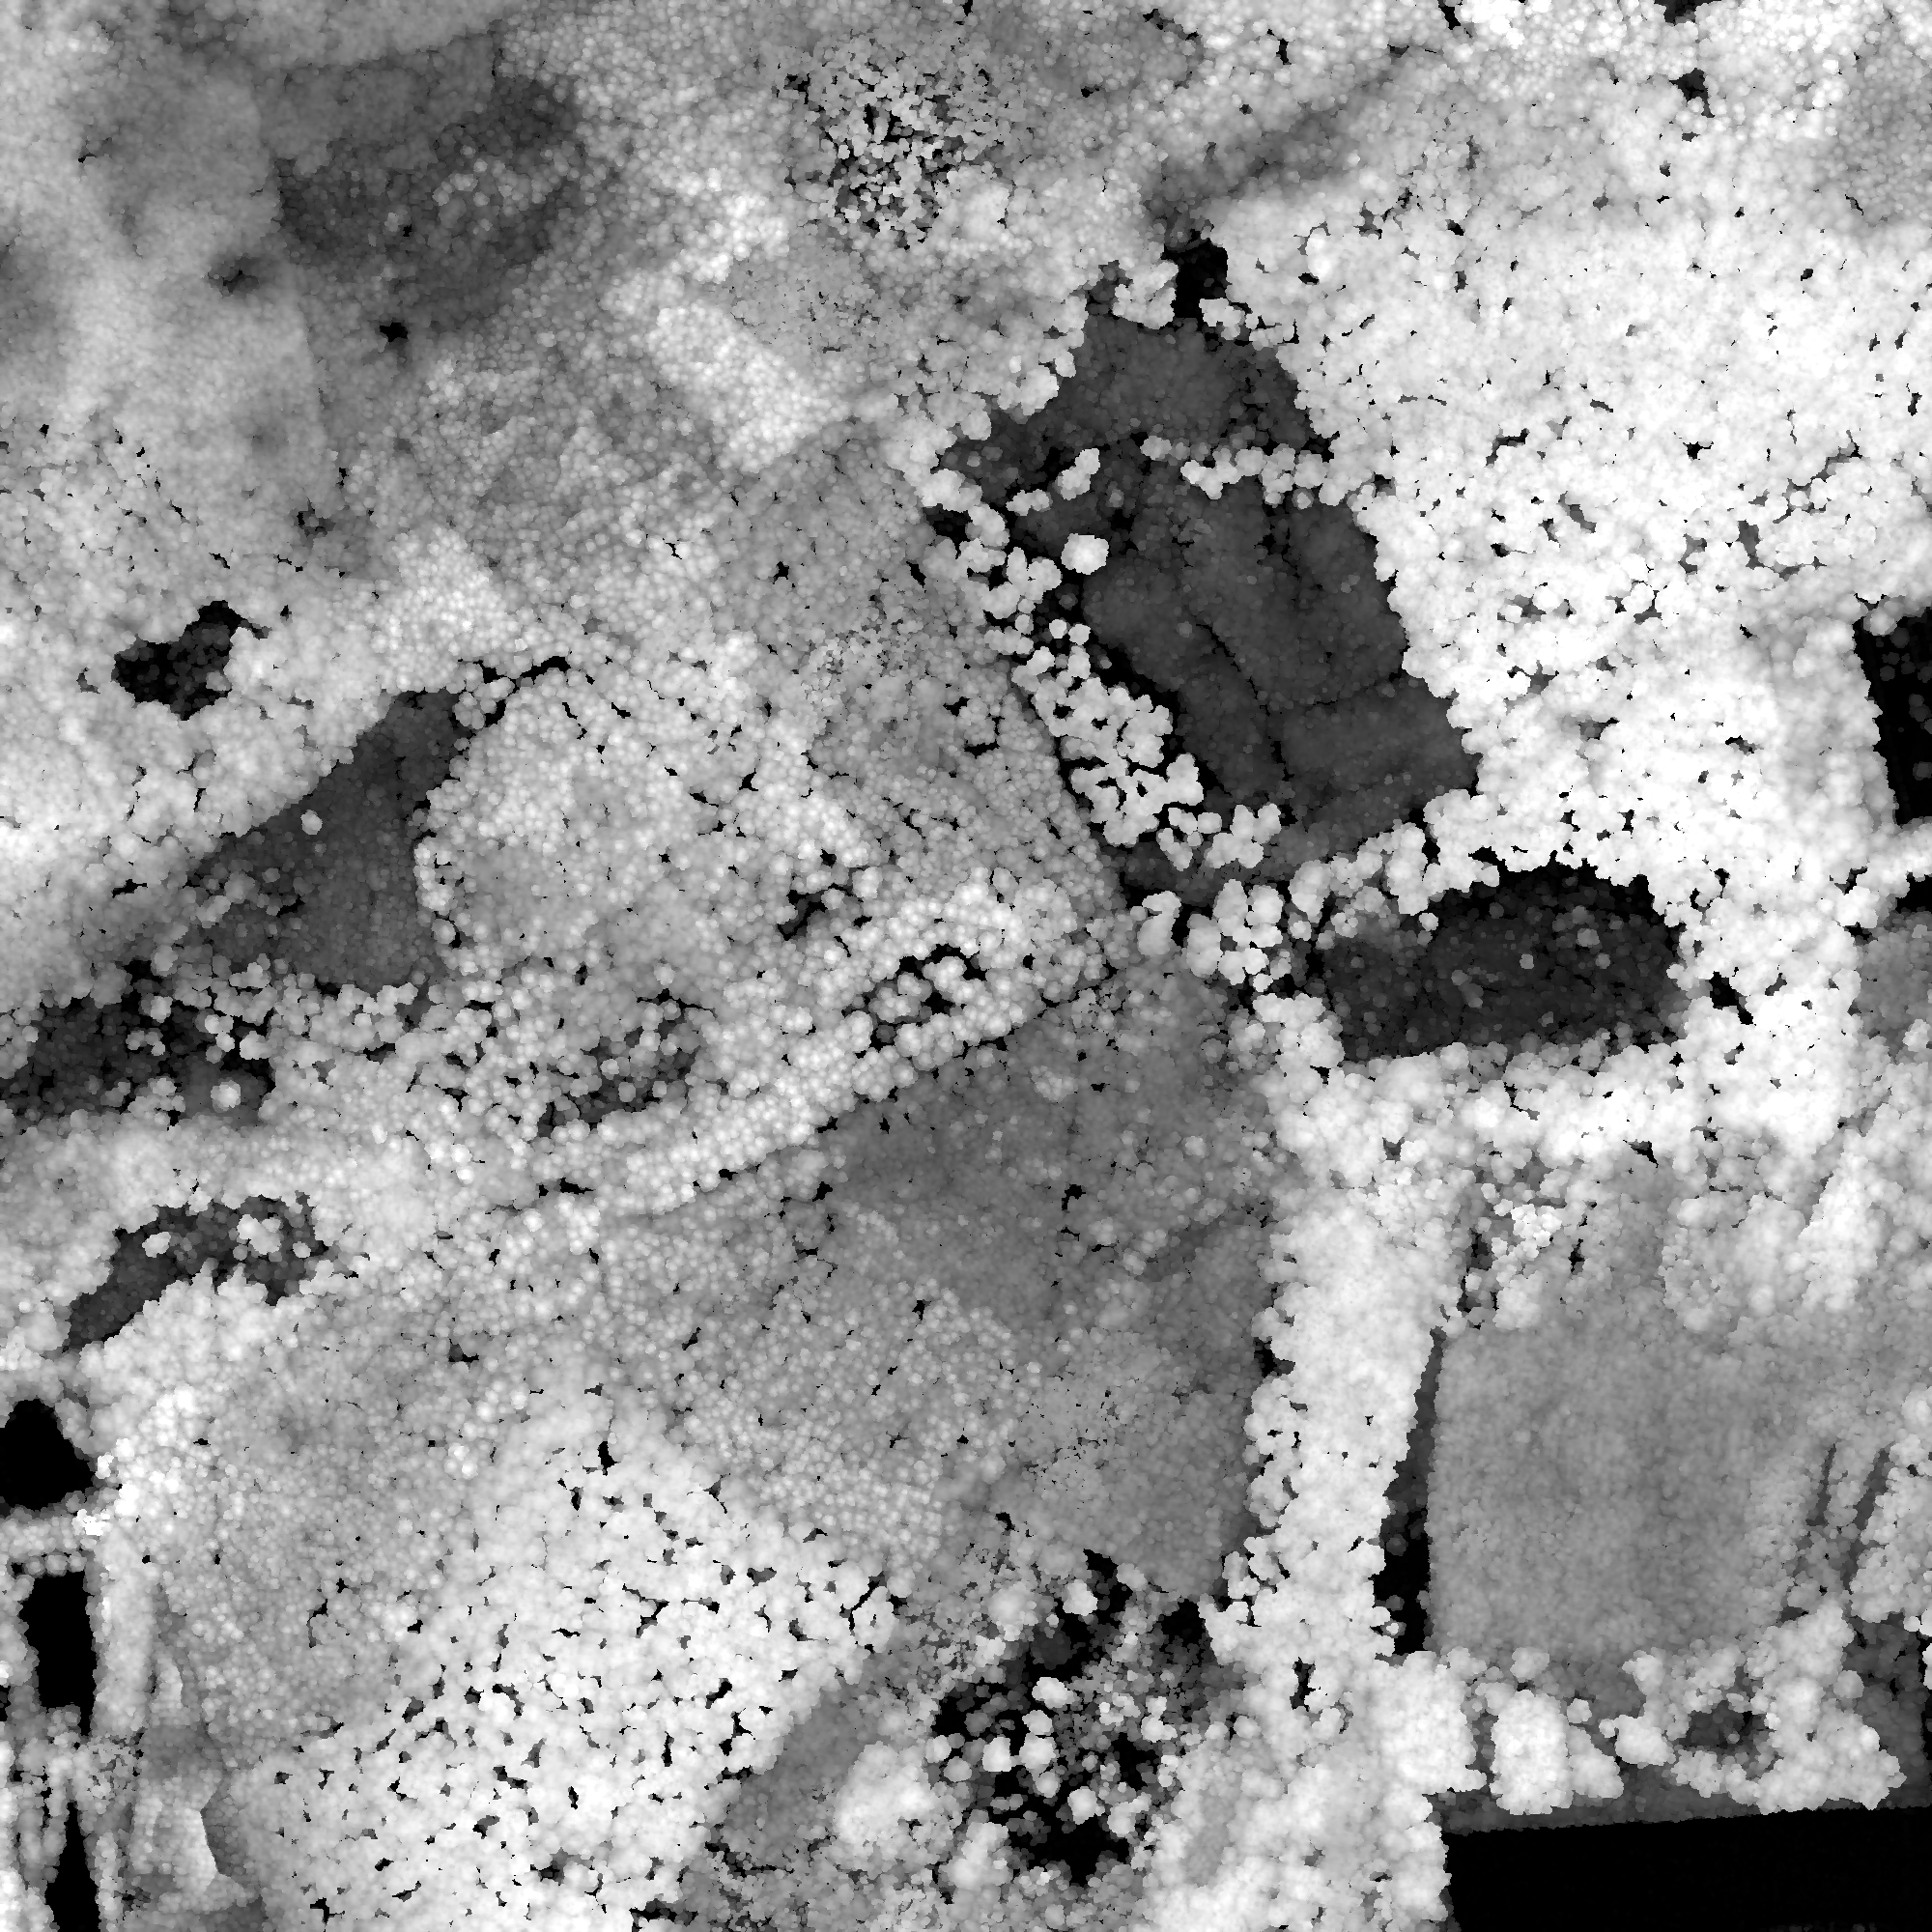
\includegraphics[width=0.45\textwidth]{Figures/C3/S3/ss3/nDSM}
\label{subfig:C3_S3_ss3_selb}
}
\\
\subfloat[Forest LC.]{
\includegraphics[width=0.45\textwidth]{Figures/C3/S3/ss3/BD}
\label{subfig:C3_S3_ss_selc}
}
\hspace*{0.025\textwidth}
\subfloat[Retained pixels for training.]{
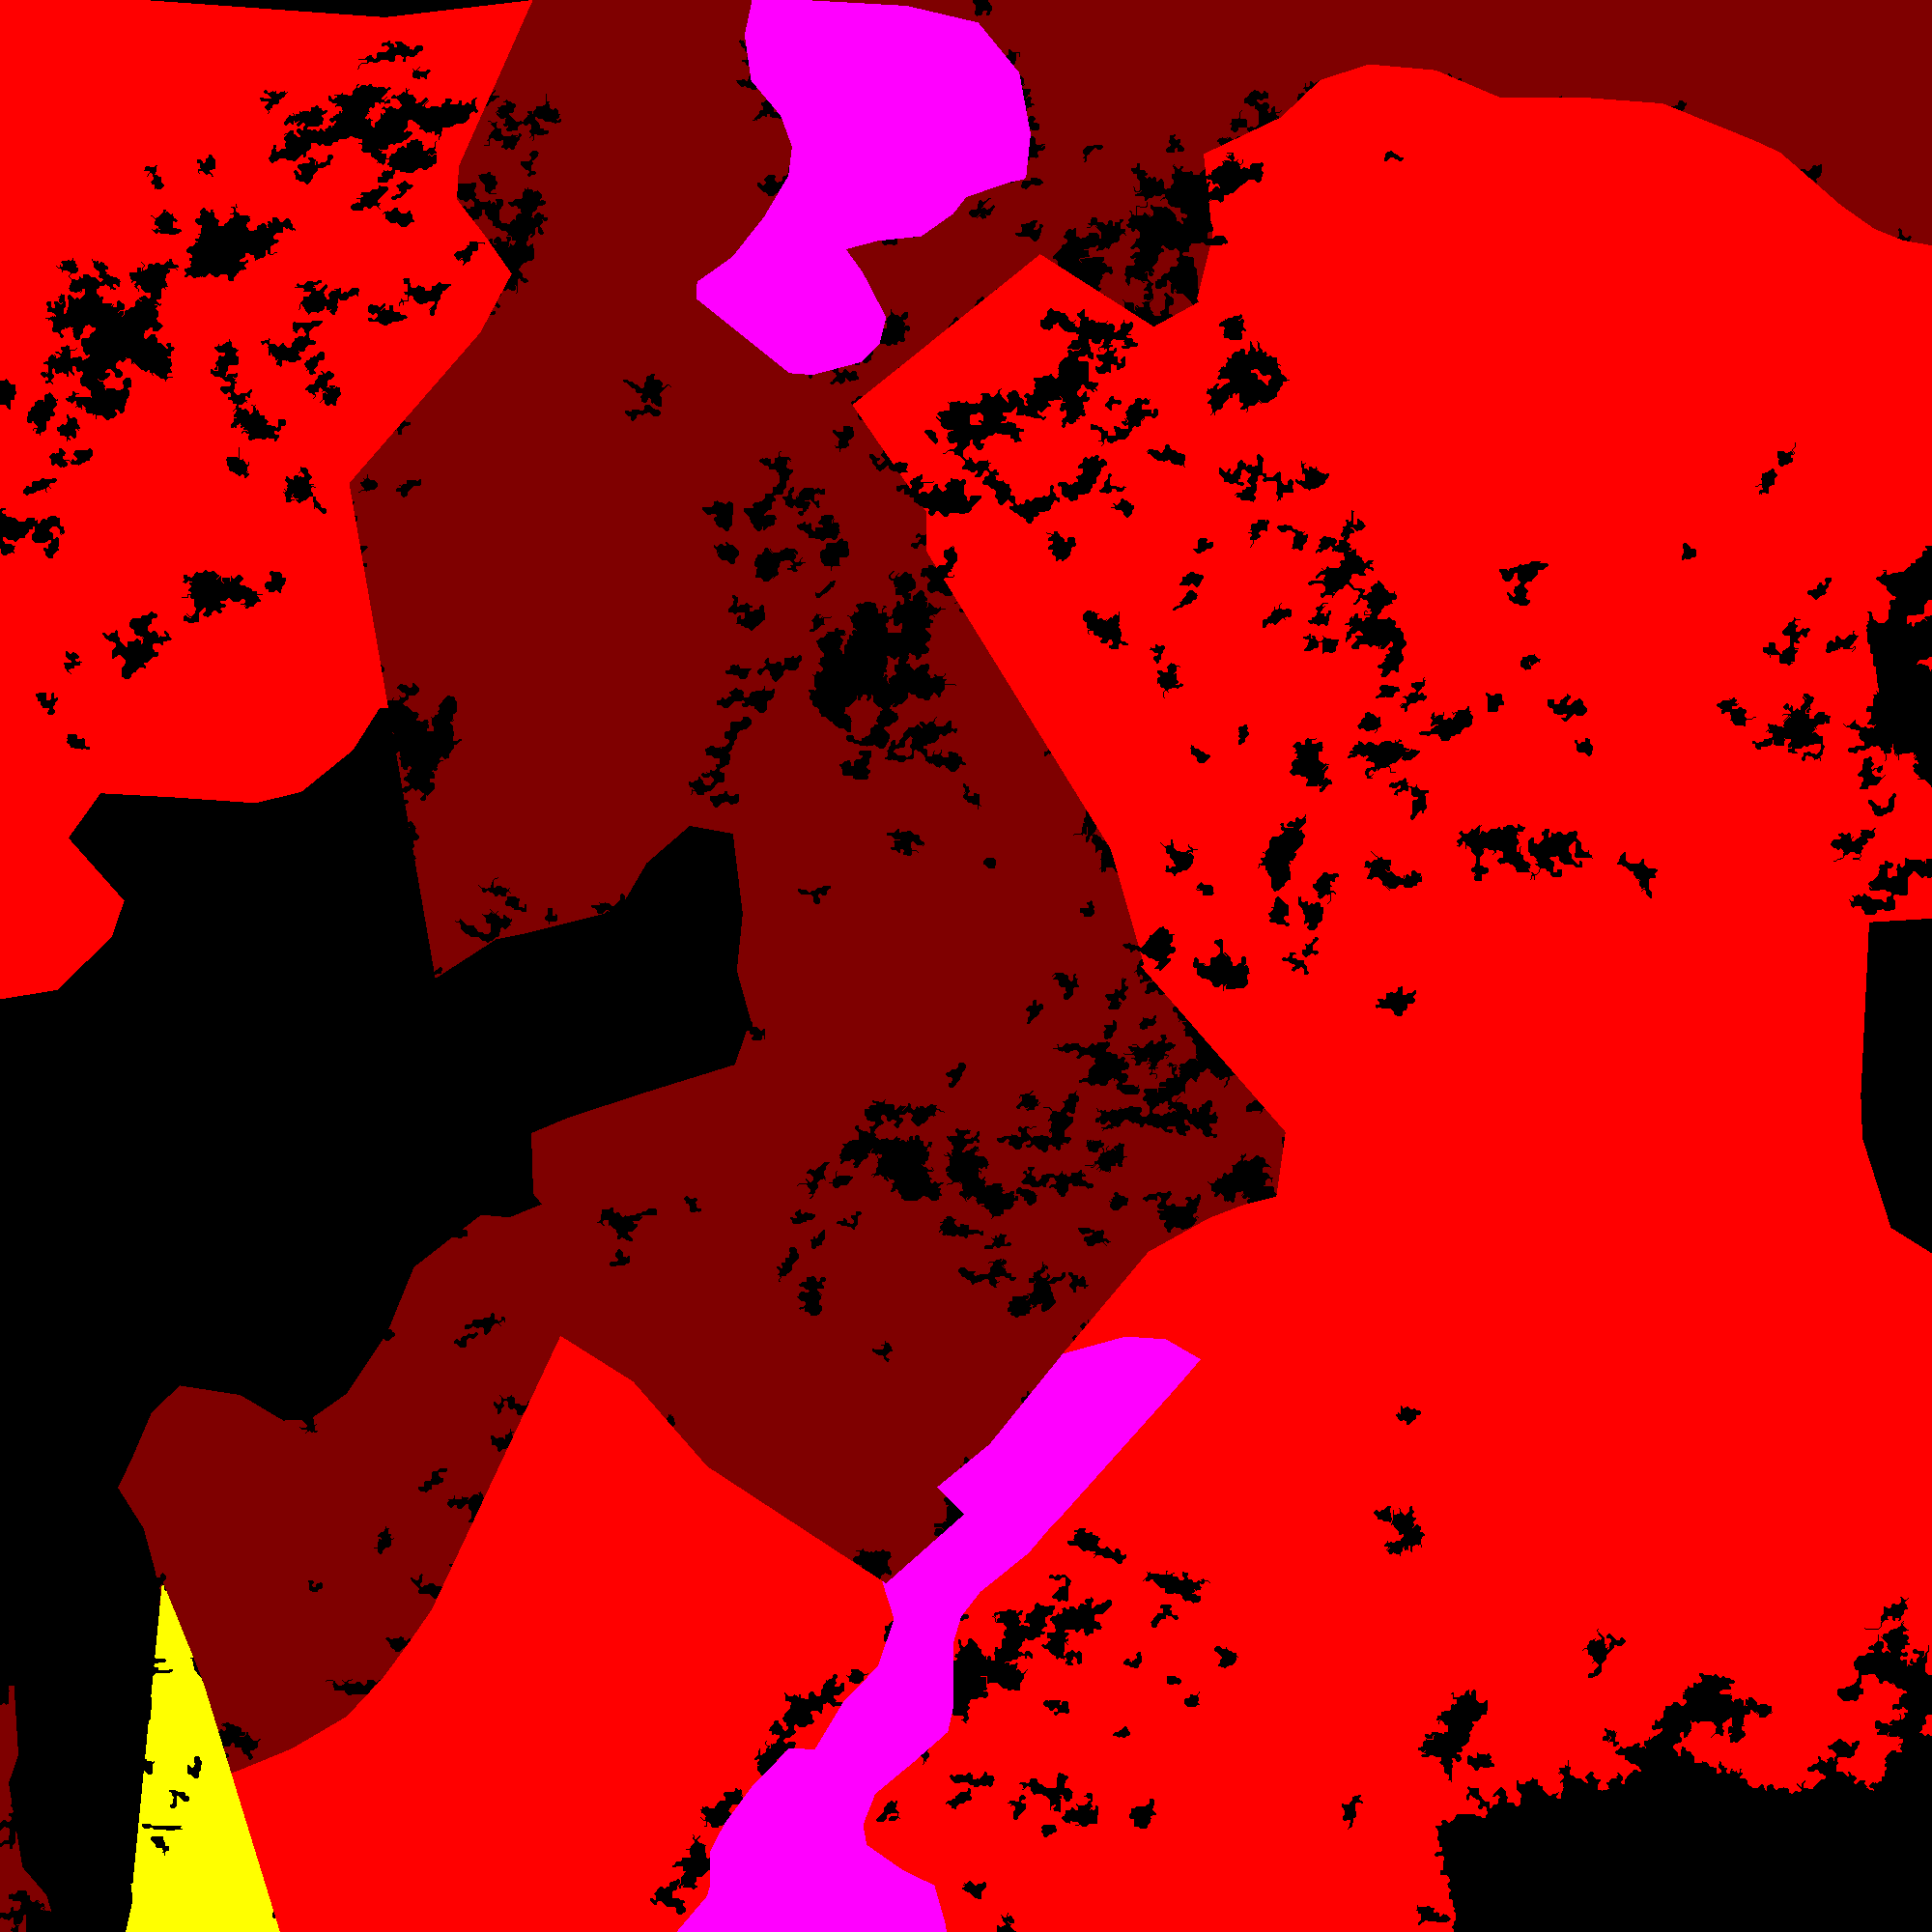
\includegraphics[width=0.45\textwidth]{Figures/C3/S3/ss3/training_set}
\label{subfig:C3_S3_ss3_seld}
}
\endgroup
\caption{Selection of the training pixels.}
\label{fig:C3_S3_ss3_sel}
\end{center}
\end{figure}

The results of the classification and regularization using different training set is presented in Figure~\ref{fig:C3_S3_ss3_sel_results}. The confusion matrices and accuracy metrics when the training pixels are not selected are presented in Tables~\ref{table:C3_S3_ss3_classif_without_training} and~\ref{table:C3_S3_ss3_regul_without_training}.

\begin{figure}[htbp]
\begin{center}
\begingroup
\captionsetup[subfigure]{width=0.45\textwidth}
\subfloat[Classification with selection of training pixels  (overall accuracy: 93.14\%, $\kappa$: 0.86).]{
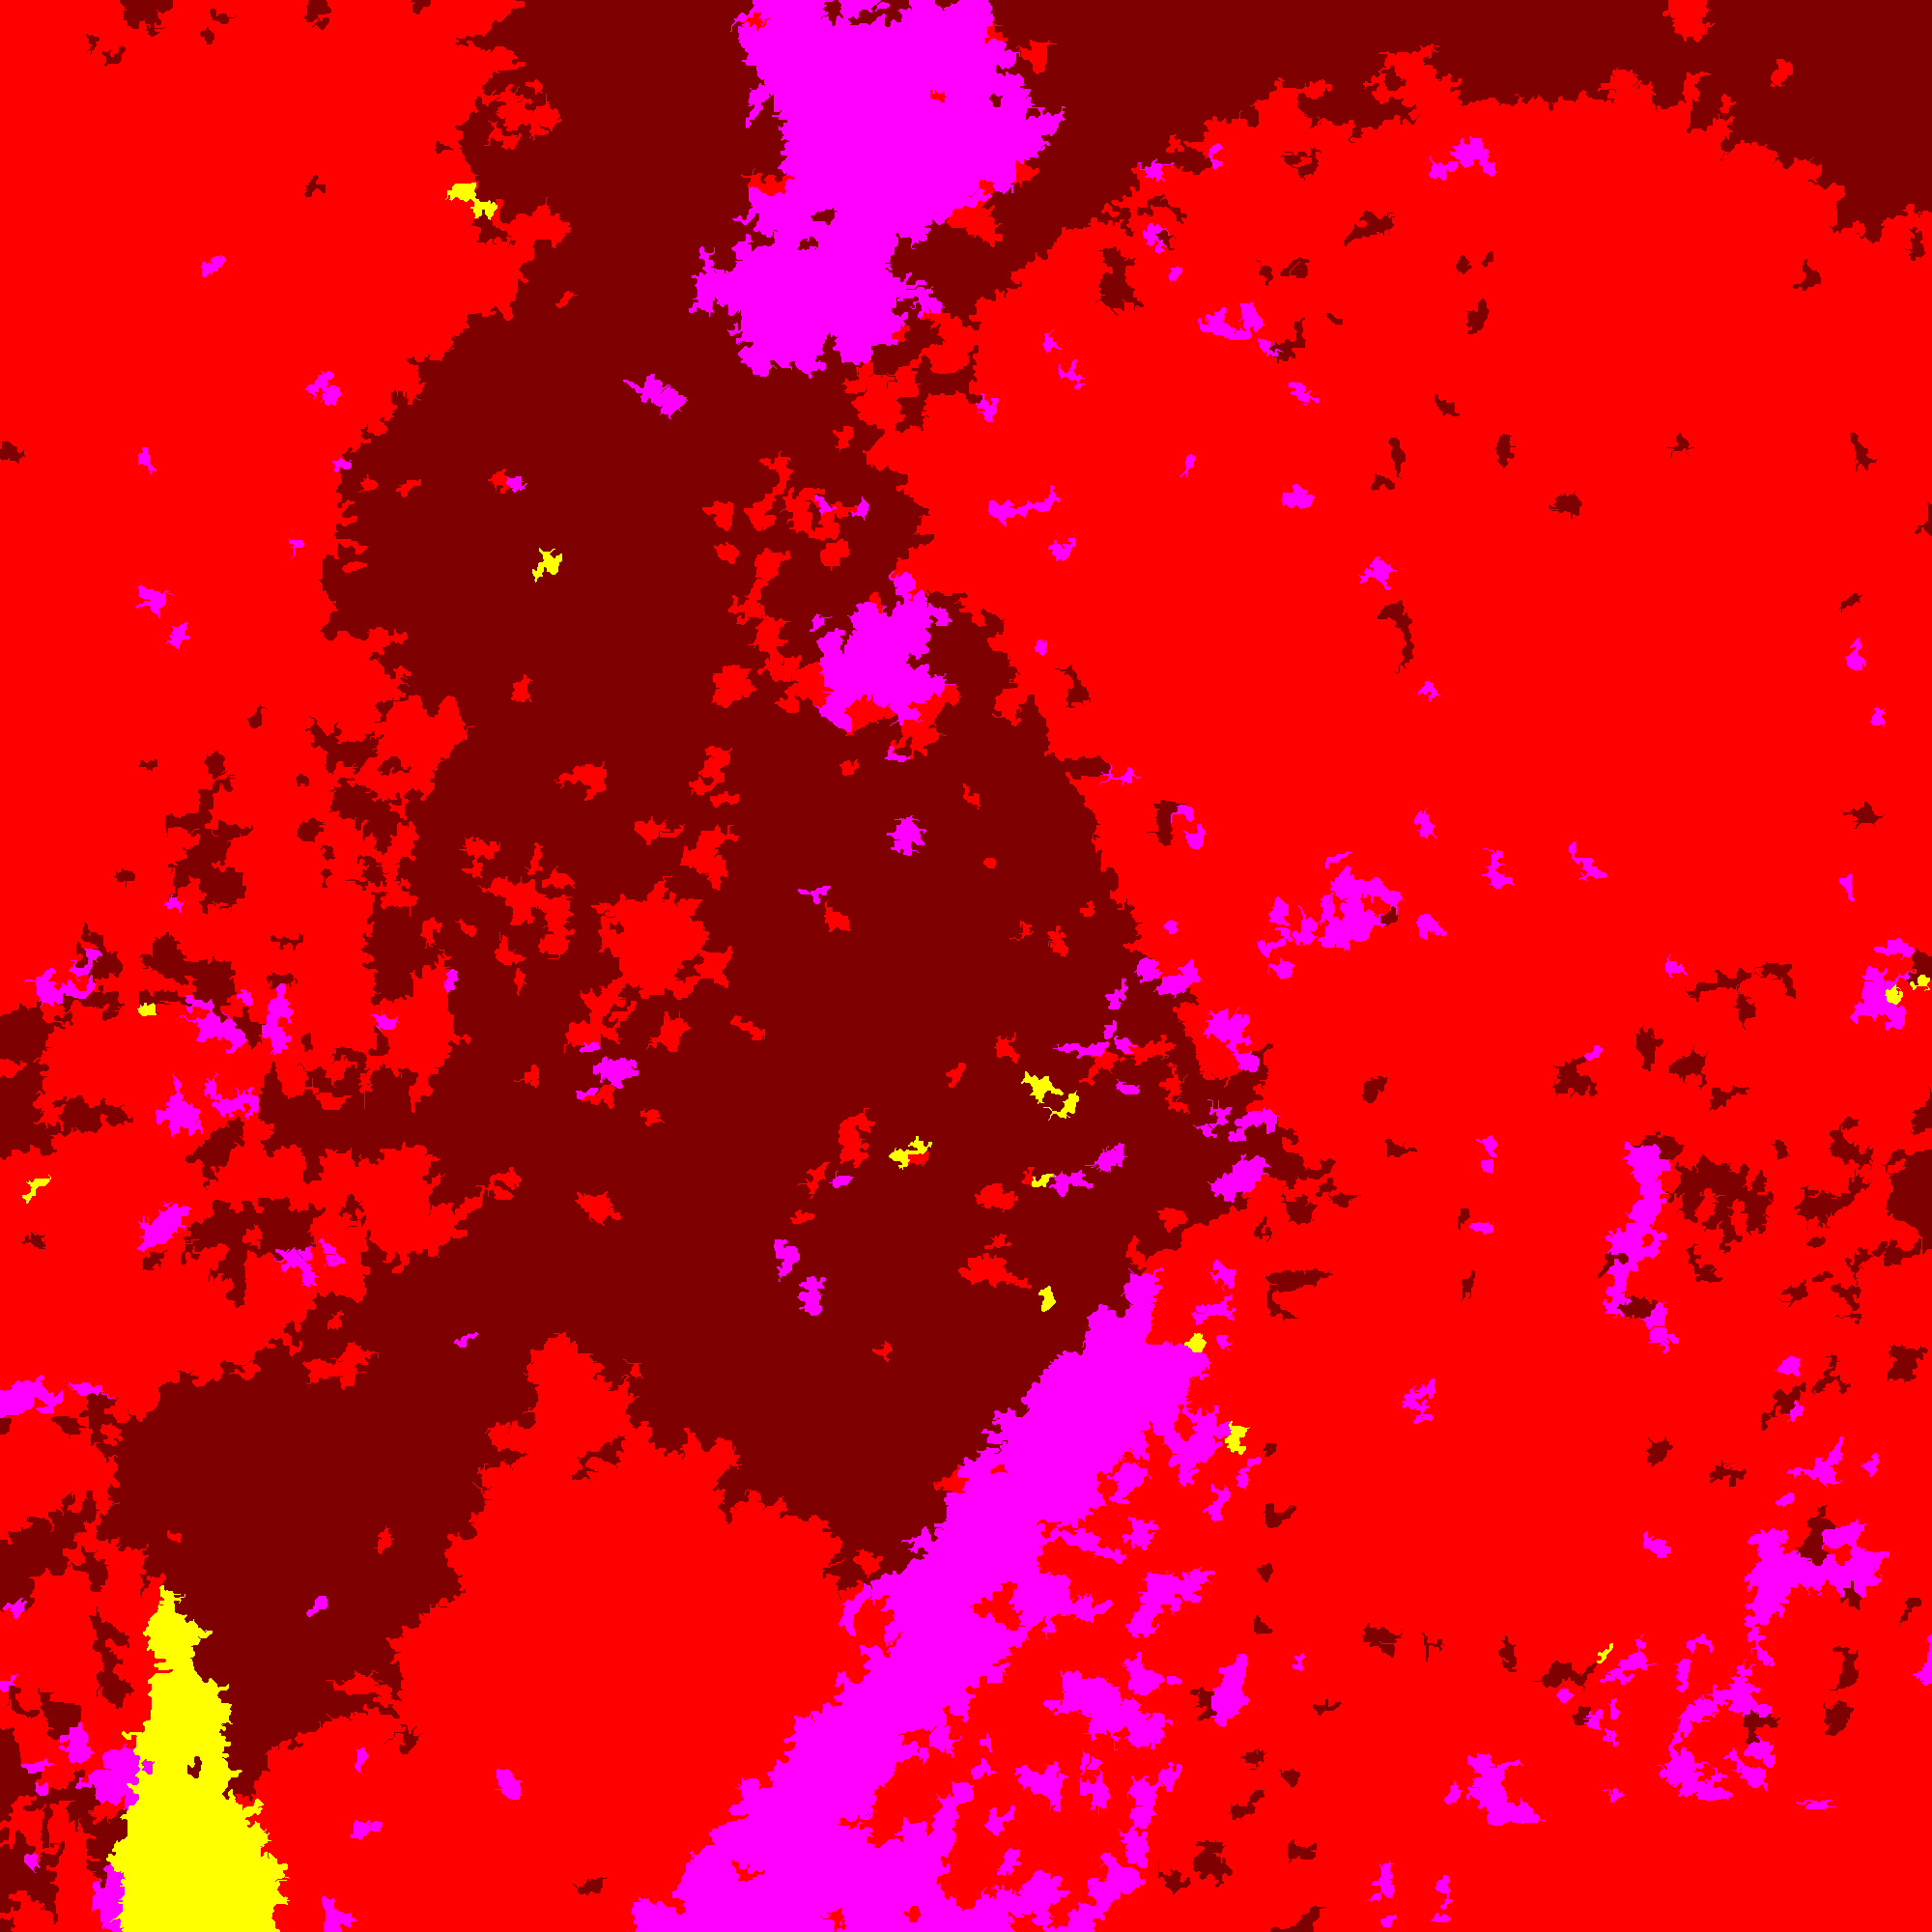
\includegraphics[width=0.45\textwidth]{Figures/C3/S3/ss3/classif_PFF}
\label{subfig:C3_S3_ss3_sel_resultsa}
}
\hspace*{0.025\textwidth}
\subfloat[Regularization  with selection of training pixels (overall accuracy: 97.44\%, $\kappa$: 0.95).]{
\includegraphics[width=0.45\textwidth]{Figures/C3/S3/ss3/regul_PFF}
\label{subfig:C3_S3_ss3_sel_resultsb}
}
\\
\subfloat[Classification without selection of training pixels (overall accuracy: 78.98\%, $\kappa$: 0.62).]{
\includegraphics[width=0.45\textwidth]{Figures/C3/S3/ss3/classif_without_training}
\label{subfig:C3_S3_ss3_sel_resultsc}
}
\hspace*{0.025\textwidth}
\subfloat[Regularization without selection of training pixels (overall accuracy: 94.67\%, $\kappa$: 0.89).]{
\includegraphics[width=0.45\textwidth]{Figures/C3/S3/ss3/regul_without_training}
\label{subfig:C3_S3_ss3_sel_resultsd}
}
\endgroup
\caption{Selection of the training pixels.}
\label{fig:C3_S3_ss3_sel_results}
\end{center}
\end{figure}

The selection of training pixels greatly increases the classification results. Indeed, without any selection, the classification is very noisy (even when working at the object level) and many confusion are reported. The regularization attenuates the errors, but the result remains worse than the one obtained with the selection of training pixels.

\subsection{Regularization}
The smoothing of the classification can be performed using local or global methods.

\subsubsection{Local methods}
Two methods have been investigated for the local smoothing of the classification. They are very easy to implement and have low computation times.
Firstly, the use of a majority filter have been employed. Since it does not take into account the probabilities, a probabilistic relaxation have then also been tested. For both method, the main problem is to defined a relevant neighborhood size. If if is too small, the results will remain noisy, and if it is too important, the results will be over generalized and the computational times will explode.

\paragraph{Majority filter. \\}
The results for the majority filter is presented in Figure~\ref{fig:C3_S3_ss4_maj}.  The filtering method performs the worse with a gain of less than 1\% compared to the classification, even with large filters. Furthermore,the larger the filter is,the longer are the computation times. 

\begin{figure}[htbp]
\begin{center}
\begingroup
\captionsetup[subfigure]{width=0.3\textwidth}
\subfloat[Forest LC database.]{
\includegraphics[width=0.3\textwidth]{Figures/C3/S3/ss4/BD}
\label{subfig:C3_S3_ss4_maja}
}
\hspace*{0.025\textwidth}
\subfloat[Majority filter ($r=5$).]{
\includegraphics[width=0.3\textwidth]{Figures/C3/S3/ss4/local/filter/5/filter}
\label{subfig:C3_S3_ss4_majb}
}
\hspace*{0.025\textwidth}
\subfloat[Majority filter ($r=25$).]{
\includegraphics[width=0.3\textwidth]{Figures/C3/S3/ss4/local/filter/25/filter}
\label{subfig:C3_S3_ss4_majc}
}
\endgroup
\caption{Results of the majority filters.}
\label{fig:C3_S3_ss4_maj}
\end{center}
\end{figure}

\paragraph{Probabilistic relaxation. \\}
The results for the probabilistic relaxation is presented in Figure~\ref{fig:C3_S3_ss4_prob}. The probabilistic relaxation has also poor results (+5\% than the classification) and has also important computation times, since the iterative process runs until the convergence has been reached.

\begin{figure}[htbp]
\begin{center}
\begingroup
\captionsetup[subfigure]{width=0.425\textwidth}
\subfloat[Forest LC database.]{
\includegraphics[width=0.45\textwidth]{Figures/C3/S3/ss4/BD}
\label{subfig:C3_S3_ss4_proba}
}
\hspace*{0.025\textwidth}
\subfloat[Probabilistic relaxation ($r=5$).]{
\includegraphics[width=0.45\textwidth]{Figures/C3/S3/ss4/local/relax/relax}
\label{subfig:C3_S3_ss4_probb}
}
\endgroup
\caption{Results of the probabilistic relaxation.}
\label{fig:C3_S3_ss4_prob}
\end{center}
\end{figure}

\subsubsection{Global methods}
The regularization is the final step that smooth the former classification. In the formulation of the energy, 3 aspect are taken into account. The two most important are the integration of the information from the classification (unary term) and how the feature are integrated into the smoothing process (prior). The last aspect is the integration of other constraints, allowed by the use of the QPBO algorithm.

The global methods produce significantly better results than the local methods.

The effect of the parameter $\gamma$ is presented in Figure~\ref{fig:C3_S3_ss4_gamma}. When $\gamma$ is low, the borders are rough and small regions might appear (Figure~\ref{subfig:C3_S3_ss4_gammac}). Increasing $\gamma$ smooth the borders, however, a too high value have a negative impact on the results, reducing the size of meaningful segments (Figure~\ref{subfig:C3_S3_ss4_gammae}) or even removing them (Figure~\ref{subfig:C3_S3_ss4_gammaf}). The tuning of the parameter $\gamma$ is an important issue, since different values of $\gamma$ might be acceptable depending on the level of detail expected for the segmentation. In forest inventory, having small regions of pure species is interesting for the understanding of the behavior of the forest. For generalization purposes (such as forest LC), the segments must have a decent size and may exhibit variability.

\begin{figure}[htbp]
\begin{center}
\begingroup
\captionsetup[subfigure]{width=0.45\textwidth}
\subfloat[IRC VHR optical image.]{
\includegraphics[width=0.45\textwidth]{Figures/C3/S3/ss4/IRC}
\label{subfig:C3_S3_ss4_gammaa}
}
\hspace*{0.025\textwidth}
\subfloat[Forest LC.]{
\includegraphics[width=0.45\textwidth]{Figures/C3/S3/ss4/BD}
\label{subfig:C3_S3_ss4_gammab}
}
\\
\subfloat[Regularization ($\gamma=5$).]{
\includegraphics[width=0.45\textwidth]{Figures/C3/S3/ss4/gamma/5/regul}
\label{subfig:C3_S3_ss4_gammac}
}
\hspace*{0.025\textwidth}
\subfloat[Regularization ($\gamma=10$).]{
\includegraphics[width=0.45\textwidth]{Figures/C3/S3/ss4/gamma/10/regul}
\label{subfig:C3_S3_ss4_gammad}
}
\\
\subfloat[Regularization ($\gamma=15$).]{
\includegraphics[width=0.45\textwidth]{Figures/C3/S3/ss4/gamma/15/regul}
\label{subfig:C3_S3_ss4_gammae}
}
\hspace*{0.025\textwidth}
\subfloat[Regularization ($\gamma=20$).]{
\includegraphics[width=0.45\textwidth]{Figures/C3/S3/ss4/gamma/20/regul}
\label{subfig:C3_S3_ss4_gammaf}
}
\endgroup
\caption{Regularization results, effect of the parameter $\gamma$.}
\label{fig:C3_S3_ss4_gamma}
\end{center}
\end{figure}

\paragraph{Unary term. \\}

The unary term have the major impact on the regularization results (see Figure~\ref{fig:C3_S3_ss4_unary}). Indeed, the log-inverse formulation highly penalize pixels with low probability, thus, small areas with high probabilities will be kept, even with an important $\gamma$. Contrarily, the linear formulation have a stronger smoothing effect.

\begin{figure}[htbp]
\begin{center}
\begingroup
\captionsetup[subfigure]{width=0.3\textwidth}
\subfloat[Forest LC database.]{
\includegraphics[width=0.3\textwidth]{Figures/C3/S3/ss4/BD}
\label{subfig:C3_S3_ss4_unarya}
}
\hspace*{0.025\textwidth}
\subfloat[Regularization results using the log-inverse data formulation.]{
\includegraphics[width=0.3\textwidth]{Figures/C3/S3/ss4/data/log/regul}
\label{subfig:C3_S3_ss4_unaryb}
}
\hspace*{0.025\textwidth}
\subfloat[Regularization results using the linear data formulation.]{
\includegraphics[width=0.3\textwidth]{Figures/C3/S3/ss4/data/linear/regul}
\label{subfig:C3_S3_ss4_unaryc}
}
\endgroup
\caption{Impact of the formulation of the unary term.}
\label{fig:C3_S3_ss4_unary}
\end{center}
\end{figure}

Both are interesting for the analysis of forest. The log-inverse allows to obtain small areas that keep an important class confidence. Such areas are useful for forest inventory since they give information about large forested areas with small islets of pure species. Conversely, the linear formulation produces smooth segments that are more relevant for a national mapping.

\paragraph{Prior. \\}

The prior have a weak impact on the regularization results (see Figure~\ref{fig:C3_S3_ss4_prior}).

\begin{figure}[htbp]
\begin{center}
\begingroup
\captionsetup[subfigure]{width=0.3\textwidth}
\subfloat[Forest LC database.]{
\includegraphics[width=0.3\textwidth]{Figures/C3/S3/ss4/BD}
\label{subfig:C3_S3_ss4_priora}
}
\hspace*{0.025\textwidth}
\subfloat[Regularization results using the \textit{Potts model}.]{
\includegraphics[width=0.3\textwidth]{Figures/C3/S3/ss4/binary/potts/regul}
\label{subfig:C3_S3_ss4_priorb}
}
\hspace*{0.025\textwidth}
\subfloat[Regularization results using the \textit{z-Potts model}.]{
\includegraphics[width=0.3\textwidth]{Figures/C3/S3/ss4/binary/cs/regul}
\label{subfig:C3_S3_ss4_priorc}
}
\\
\subfloat[Regularization results using the \textit{Exponential-features model}.]{
\includegraphics[width=0.3\textwidth]{Figures/C3/S3/ss4/binary/ef/regul}
\label{subfig:C3_S3_ss4_priord}
}
\hspace*{0.025\textwidth}
\subfloat[Regularization results using the \textit{Distance-features model}.]{
\includegraphics[width=0.3\textwidth]{Figures/C3/S3/ss4/binary/df/regul}
\label{subfig:C3_S3_ss4_priore}
}
\endgroup
\caption{Impact of the formulation of the data term.}
\label{fig:C3_S3_ss4_prior}
\end{center}
\end{figure}

The \textit{z-Potts model} tends to have slightly worse results than the other methods. The \textit{Potts model} and the \textit{Distance-features model} have very close results regardless of the unary term. The \textit{Exponential-features model} have the greatest results with the linear unary, but have poor results with the log-inverse unary.

\paragraph{Adding constraints. \\}
The addition of constraints could be easily carried out with the QPBO algorithm. We can add strong borders that we want to retrieve in the final segmentation. Unfortunately, such borders can not be easily extracted (see Section~\ref{sec:C3_S2_ss1}). It is then not relevant to add such constraints since they will not lead to accurate results. 

A second constraint can be employed in order to ensure a minimal size of the final segments. However, it leads to three issues
\begin{enumerate}
\item The minimal size of a segment should be defined. Even if such minimal size is defined by the definition of forest stands (0.5$\:$ha), a segment with a size of 0.5$\:$ha$+$1 pixels will not be considered as a small segment.
\item If such constraint wants to be employed, the QPBO algorithm have to run until all the segments have reached the minimum size. Such iteration might be long
\item The final result will be similar to a majority vote. For a small segment, selecting the label of the neighbor segment that have the most neighbor pixels with the small segment will nearly lead to the same results of the regularization using minimal size constraint.
\end{enumerate}

\subsection{Importance of fusion}
In this framework, the fusion is performed at multiple levels;
\begin{itemize}
\item Choice of data for the over-segmentation,
\item Features employed for the classification,
\item Features employed for the regularization.
\end{itemize}

The impact of the choice of the data for the over-segmentation have already been investigated in Section~\ref{sec:C3_S3_ss1}. When employing an over-segmentation from VHR optical images (e.g. PFF, Quickshift or SLIC) or from a lidar data (e.g. hierarchical segmentation on nDSM or tree extraction) produces similar results. 

Experiments have been conducted in order to determine how the choice of the data impact both the classification and regularization step. In order to evaluate the impact of the data choice on the classification and regularization, 5 scenarii have been investigated:
\begin{itemize}
\item A full lidar scenario:
\begin{itemize}
\item Hierarchical segmentation on the nDSm,
\item Object-based classification (with selection of training samples) using the 25 lidar features,
\item Regularization using the 25 lidar features.
\end{itemize}
\item A full spectral scenario:
\begin{itemize}
\item PFF segmentation of the VHR optical image,
\item Object-based classification (with selection of training samples) using a selection of 20 spectral features,
\item Regularization using a selection of 20 spectral features.
\end{itemize}
\item 3 scenarii:
\begin{itemize}
\item PFF segmentation of the VHR optical image,
\item Object-based classification (with selection of training samples) using a selection of 20 features (lidar and spectral),
\end{itemize}
\begin{enumerate}
\item Regularization using the 25 lidar features,
\item Regularization using a selection of 20 spectral features,
\item Regularization using a selection of 20 features (lidar and spectral).
\end{enumerate}
\end{itemize}

The overall accuracies for these 5 scenarii are presented in Table~\ref{table:fusion_results}.

\begin{table}[htbp]
\begin{center}
\begin{footnotesize}
\begin{tabular}{|l|c|c|c|}
\hline
\multirow{2}{*}{Scenario} & \multicolumn{3}{c|}{\textbf{Overall accuracy (\%)}} \\
\cline{2-4}
& Classification & Regularization & Gain \\
\hline
Full lidar & 74.8 & 92.2 & 17.4 \\
\hline
Full spectral & 79.1 & 95.2 & 16.1 \\
\hline
Regularization lidar & \multirow{3}{*}{87.6} & 96.0 & 8.4 \\
\cline{1-1} \cline{3-4}
Regularization spectral &  & 96.1 & 8.5 \\
\cline{1-1} \cline{3-4}
Regularization lidar + spectral &  & 96.2 & 8.6 \\
\hline
\end{tabular} \\
\end{footnotesize}
\end{center}
\vspace*{-5mm}
\caption{Classification and stand segmentation accuracies for the 5 scenarii investigated.}
\label{table:fusion_results}
\end{table}

The impact of the choice of the data on the classification is obvious; the classification using a single data source performs worse than when using both. Furthermore, the spectral information tends to be more relevant that the spectral information. Such results are coherent with the results of the feature selection since the spectral feature are selected for 61\% and for 39\% for the lidar.

The impact of the choice of the data on the regularization is less significant. We can first note that the use of a single modality can greatly improve the results from a poor classification (+17.4\% for lidar and +16.1\% for spectral). However, when the classification is already significant, the improvement is more or less the same. The spectral information is a bit more beneficial than the lidar information for the regularization step. Fusing the two data sources or using only the spectral information in the regularization step does not significantly change the final results.

\section{Co-products of the method}
The outputs of the method can be employed for further investigation in order to extract relevant information about forest. Firstly, the forest stands obtained can be employed for the semi-automatic update of the forest LC. Secondly, the information extracted from the original data can be employed for forest inventory.
\subsection{Semi-automatic update}
The semi-automatic update of the forest LC can be performed by the joint analysis of the final stand segmentation and the forest LC employed.

A change map can be derived and changes can be prioritized according to their size and shape.
Here 3 criteria are employed for an area of change :
\begin{itemize}
\item The number of pixels,
\item The size of the rectangular bounding box (see Figure~\ref{subfig:changesb}),
\item The size of the circular bounding box (see Figure~\ref{subfig:changesc}).
\end{itemize}

\begin{figure}[htbp]
\begin{center}
\begingroup
\captionsetup[subfigure]{width=0.3\textwidth}
\subfloat[Detected change]{
\includegraphics[width=0.3\textwidth]{Figures/C3/S4/ss1/area}
\label{subfig:changes}
}
\hfill
\subfloat[Rectangular bounding box of the change.]{
\includegraphics[width=0.3\textwidth]{Figures/C3/S4/ss1/area_rectangular}
\label{subfig:changesb}
}
\hfill
\subfloat[Circular bounding box of the change.]{
\includegraphics[width=0.3\textwidth]{Figures/C3/S4/ss1/area_circular}
\label{subfig:changesc}
}
\endgroup
\caption{Bounding boxes of the change detection.}
\label{fig:changes}
\end{center}
\end{figure}

The changes are classified using thresholds based on the size (in pixels) of the change $s$, the ratio between the size of the change and the size of the rectangular bounding box $r_{1}$ and  the ratio between the size of the change and the size of the circular bounding box $r_{2}$. An change is defined as major when the condition~(\ref{eq:c1}) or~(\ref{eq:c2}) is verified. 
\begin{eqnarray}
s \geq 100 \text{ and } r_{1} \geq 0.3, \label{eq:c1}\\
s \geq 100 \text{ and } r_{2} \geq 0.2. \label{eq:c2}
\end{eqnarray}

An "updated" forest LC can be then created, the area of major change are labeled as \textit{no data} (see Figure~\ref{fig:new_BD}). A difference map is also produced with two kinds of differences:
\begin{itemize}
\item The minor differences; they correspond to areas where the borders of the Forest LC does not exactly fit with the borders obtained in the method. This type of error is common since the border from the Forest LC are mostly strait lines while the methods tends to follow the natural borders of the forest because of the regularization.
\item The major differences; they correspond to large patches that differ from the Forest LC. Two cases can be differentiated:
\begin{itemize}
\item The method can have produced wrong results,
\item The forest has changed or has been exploited (cut or plantation).
\end{itemize}
\end{itemize}

\begin{figure}[htbp]
\begin{center}
\begingroup
\captionsetup[subfigure]{width=0.5\textwidth}
\subfloat[Forest LC.]{
\includegraphics[width=0.45\textwidth]{Figures/C3/S4/ss1/results/BD}
\label{subfig:new_BDa}
}
\hfill
\subfloat["Updated" Forest LC.]{
\includegraphics[width=0.45\textwidth]{Figures/C3/S4/ss1/results/BD_new}
\label{subfig:new_BDb}
}
\endgroup
\caption{Automatic update of the Forest LC.}
\label{fig:new_BD}
\end{center}
\end{figure}

In case of major change, the decision can be taken to keep the original forest LC or to employ the result of the method. An operator can also focus of the change and correct it manually (see Figure~\ref{fig:IRC_change})

\begin{figure}[htbp]
\begin{center}
\includegraphics[width=1.0\textwidth]{Figures/C3/S4/ss1/results/IRC_dif}
\caption{Detected changes of the Forest LC, green corresponds to major changes, blue corresponds to minor changes.}
\label{fig:IRC_change}
\end{center}
\end{figure}

\subsection{Inventory}
The features derived from lidar and the final stand segmentation

%----------------------------------------------------------------------------------------

% Define some commands to keep the formatting separated from the content 
%\newcommand{\keyword}[1]{\textbf{#1}}
%\newcommand{\tabhead}[1]{\textbf{#1}}
%\newcommand{\code}[1]{\texttt{#1}}
%\newcommand{\file}[1]{\texttt{\bfseries#1}}
%\newcommand{\option}[1]{\texttt{\itshape#1}}

%----------------------------------------------------------------------------------------


\stopcontents[chapters]